% !TeX spellcheck = de-DE
% !TeX encoding = utf8
% !TeX program = lualatex
% !BIB program = biber
% -*- coding:utf-8 mod:LaTeX -*-

% vv  scroll down to line 200 for content  vv


\let\ifdeutsch\iftrue
\let\ifenglisch\iffalse
% EN: This file is loaded before the \documentclass command in the main document

% EN: The following package allows \\ at the title page
%     For more information see https://github.com/latextemplates/scientific-thesis-cover/issues/4
\RequirePackage{kvoptions-patch}

\ifenglisch
  \PassOptionsToClass{numbers=noenddot}{scrbook}
\else
  %()Aus scrguide.pdf - der Dokumentation von KOMA-Script)
  %Nach DUDEN steht in Gliederungen, in denen ausschließlich arabische Ziffern für die Nummerierung
  %verwendet werden, am Ende der Gliederungsnummern kein abschließender Punkt
  %(siehe [DUD96, R3]). Wird hingegen innerhalb der Gliederung auch mit römischen Zahlen
  %oder Groß- oder Kleinbuchstaben gearbeitet, so steht am Ende aller Gliederungsnummern ein
  %abschließender Punkt (siehe [DUD96, R4])
  \PassOptionsToClass{numbers=autoendperiod}{scrbook}
\fi

% Warns about outdated packages and missing caption declarations
% See https://www.ctan.org/pkg/nag
\RequirePackage[l2tabu, orthodox]{nag}

%DE: Neue deutsche Trennmuster
%    Siehe http://www.ctan.org/pkg/dehyph-exptl und http://projekte.dante.de/Trennmuster/WebHome
%    Nur für pdflatex, nicht für lualatex
\RequirePackage{ifluatex}
\ifluatex
  % do not load anything
\else
  \ifdeutsch
    \RequirePackage[ngerman=ngerman-x-latest]{hyphsubst}
  \fi
\fi

\documentclass[
  ngerman,
  % fontsize=11pt is the standard
  a4paper,  % Standard format - only KOMAScript uses paper=a4 - https://tex.stackexchange.com/a/61044/9075
  twoside,  % we are optimizing for both screen and two-side printing. So the page numbers will jump, but the content is configured to stay in the middle (by using the geometry package)
  bibliography=totoc,
  %               idxtotoc,   %Index ins Inhaltsverzeichnis
  %               liststotoc, %List of X ins Inhaltsverzeichnis, mit liststotocnumbered werden die Abbildungsverzeichnisse nummeriert
  headsepline,
  cleardoublepage=empty,
  parskip=half,
  %               draft    % um zu sehen, wo noch nachgebessert werden muss - wichtig, da Bindungskorrektur mit drin
  draft=false
]{scrbook}
% !TeX encoding = utf8
% -*- coding:utf-8 mod:LaTeX -*-

% EN: This file includes basic packages and sets options. The order of package
%     loading is important
% DE: In dieser Datei werden zuerst die benoetigten Pakete eingebunden und
%     danach diverse Optionen gesetzt. Achtung Reihenfolge ist entscheidend!


%%%
% EN: Styleguide:
% - English comments are prefixed with "EN", German comments are prefixed with "DE"
% - Prefixed headings define the language for the subsequent paragraphs
% - It is tried to organize packages in blocks. One block starts with %%%, then
%   % <heading>, then the options and more text. % followed by %%% end a block.
%
% DE: Styleguide:
%
% Ein sehr kleiner Styleguide. Packages werden in Blöcken organisiert.
% Ein Block beginnt mit drei % in einer Zeile, dann % <Blocküberschrift>, dann
% eine Liste der möglichen Optionen und deren Einstellungen, Gründe und Kommentare
% eine % Zeile in der sonst nichts steht und dann wieder %%% in einer Zeile.
%
% Zwischen zwei Blöcken sind 2 Leerzeilen!
% Zu jedem Paket werden soviele Optionen wie möglich/nötig angegeben
%
%%%


%%%
% EN: Enable copy and paste of text from the PDF
%     Only required for pdflatex. It "just works" in the case of lualatex.
%     mmap enables mathematical symbols, but does not work with the newtx font set
%     See: https://tex.stackexchange.com/a/64457/9075
%     Other solutions outlined at http://goemonx.blogspot.de/2012/01/pdflatex-ligaturen-und-copynpaste.html and http://tex.stackexchange.com/questions/4397/make-ligatures-in-linux-libertine-copyable-and-searchable
%     Trouble shooting outlined at https://tex.stackexchange.com/a/100618/9075
\ifluatex
\else
  \usepackage{cmap}
\fi
%%%


%%%
% EN: File encoding
% DE: Codierung
%     Wir sind im 21 Jahrhundert, utf-8 löst so viele Probleme.
%
% Mit UTF-8 funktionieren folgende Pakete nicht mehr. Bitte beachten!
%   * fancyvrb mit §
%   * easylist -> http://www.ctan.org/tex-archive/macros/latex/contrib/easylist/
\ifluatex
  % EN: See https://tex.stackexchange.com/a/158517/9075
  %     Not required, because of usage of fontspec package
  %\usepackage[utf8]{luainputenc}
\else
  \usepackage[utf8]{inputenc}
\fi
%
%%%

%%%
% DE: Parallelbetrieb tex4ht und pdflatex
\makeatletter
\@ifpackageloaded{tex4ht}{
  \def\iftex4ht{\iftrue}
}{
  \def\iftex4ht{\iffalse}
}
\makeatother
%%%


%%%
% EN: Defintion of colors
% DE: Farbdefinitionen
\usepackage[hyperref,dvipsnames]{xcolor}
%

%%%
% EN: Required for custom acronyms/glossaries style.
%     Left aligned Columns in tables with fixed width.
%     See http://tex.stackexchange.com/questions/91566/syntax-similar-to-centering-for-right-and-left
\usepackage{ragged2e}
%%%

%%%
% EN: Abbreviations
% DE: Abkürzungsverzeichnis
%
% DE: Wichtig, ansonsten erscheint "No room for a new \write"
\usepackage{scrwfile}
% DE: siehe http://www.dickimaw-books.com/cgi-bin/faq.cgi?action=view&categorylabel=glossaries#glsnewwriteexceeded
\usepackage[acronym,indexonlyfirst,nomain]{glossaries}
\ifdeutsch
  \renewcommand*{\acronymname}{Abkürzungsverzeichnis}
\else
  \renewcommand*{\acronymname}{List of Abbreviations}
\fi
\renewcommand*{\glsgroupskip}{}
%
% EN: Removed Glossarie as a table as a quick fix to get the template working again
%     See http://tex.stackexchange.com/questions/145579/how-to-print-acronyms-of-glossaries-into-a-table
%
\makenoidxglossaries
%%%


%%%
% EN: Support for language-specific hyphenation
% DE: Neue deutsche Rechtschreibung und Literatur statt "Literature"
%     Die folgende Einstellung ist der Nachfolger von ngerman.sty
\ifdeutsch
  % DE: letzte Sprache ist default, Einbindung von "american" ermöglicht \begin{otherlanguage}{amercian}...\end{otherlanguage} oder \foreignlanguage{american}{Text in American}
  %     Siehe auch http://tex.stackexchange.com/a/50638/9075
  \usepackage[american,ngerman]{babel}
  % Ein "abstract" ist eine "Kurzfassung", keine "Zusammenfassung"
  \addto\captionsngerman{%
    \renewcommand\abstractname{Kurzfassung}%
  }
  \ifluatex
    % EN: conditionally disable ligatures. See https://github.com/latextemplates/scientific-thesis-template/issues/54
    %     for a discussion
    \usepackage[ngerman]{selnolig}
  \fi
\else
  % EN: Set English as language and allow to write hyphenated"=words
  %     `american`, `english` and `USenglish` are synonyms for babel package (according to https://tex.stackexchange.com/questions/12775/babel-english-american-usenglish).
  %      "english" has to go last to set it as default language
  \usepackage[ngerman,english]{babel}
  % EN: Hint by http://tex.stackexchange.com/a/321066/9075 -> enable "= as dashes
  \addto\extrasenglish{\languageshorthands{ngerman}\useshorthands{"}}
  \ifluatex
    % EN: conditionally disable ligatures. See https://github.com/latextemplates/scientific-thesis-template/issues/54
    %     for a discussion
    \usepackage[english]{selnolig}
  \fi
\fi
%
%%%


%%%
% EN: For easy quotations: \enquote{text}
%     This package is very smart when nesting is applied, otherwise textcmds (see below) provides a shorter command
%     Note that this package results in a warning when it is loaded before minted (actually fvextra).
% DE: Anführungszeichen
%     Zitate in \enquote{...} setzen, dann werden automatisch die richtigen Anführungszeichen verwendet.
%     Dieses package erzeugt eine Warnung, wenn es vor minted (genauer fvextra) geladen wird.
\usepackage{csquotes}
%%%


%%%
% EN: For even easier quotations: \qq{text}.
%     Is not smart in the case of nesting, but good enough for the most cases
\usepackage{textcmds}
\ifdeutsch
  % EN: German quotes are different. So do not use the English quotes, but the ones provided by the csquotes package.
  \renewcommand{\qq}[1]{\enquote{#1}}
\fi
%%%


%%%
% EN: extended enumarations
% DE: erweitertes Enumerate
\usepackage{paralist}
%
%%%


%%%
% DE: fancyheadings (nicht nur) fuer koma
\usepackage[automark]{scrlayer-scrpage}
%
%%%


%%%
% EN: Mathematics
% DE: Mathematik
%
% DE: Viele Mathematik-Sachen. Siehe https://texdoc.net/pkg/amsmath
\usepackage{amsmath}
% EN: Options must be passed this way, otherwise it does not work with glossaries
\PassOptionsToPackage{fleqn,leqno}{amsmath}
% DE: fleqn (=Gleichungen linksbündig platzieren) funktioniert nicht direkt. Es muss noch ein Patch gemacht werden:
%\addtolength\mathindent{1em}%work-around ams-math problem with align and 9 -> 10. Does not work with glossaries, No visual changes.
% EN: Fixes bugs in AMS math
\usepackage{mathtools}
%
% EN: For theorems, replacement for amsthm
\usepackage[amsmath,hyperref]{ntheorem}
\theorempreskipamount 2ex plus1ex minus0.5ex
\theorempostskipamount 2ex plus1ex minus0.5ex
\theoremstyle{break}
\newtheorem{definition}{Definition}[section]
%
%%%


%%%
% DE: Intelligentes Leerzeichen um hinter Abkürzungen die richtigen Abstände zu erhalten, auch leere.
%     Siehe commands.tex \gq{}
\usepackage{xspace}
%DE: Macht \xspace und \enquote kompatibel
\makeatletter
\xspaceaddexceptions{\grqq \grq \csq@qclose@i \} }
\makeatother
%
%%%

\newcommand{\eg}{e.\,g.,\ }
\newcommand{\ie}{i.\,e.,\ }

% EN: introduce \powerset - hint by http://matheplanet.com/matheplanet/nuke/html/viewtopic.php?topic=136492&post_id=997377
\DeclareFontFamily{U}{MnSymbolC}{}
\DeclareSymbolFont{MnSyC}{U}{MnSymbolC}{m}{n}
\DeclareFontShape{U}{MnSymbolC}{m}{n}{
  <-6>    MnSymbolC5
  <6-7>   MnSymbolC6
  <7-8>   MnSymbolC7
  <8-9>   MnSymbolC8
  <9-10>  MnSymbolC9
  <10-12> MnSymbolC10
  <12->   MnSymbolC12%
}{}
\DeclareMathSymbol{\powerset}{\mathord}{MnSyC}{180}

%%%
% EN: Package for the appendix
% DE: Anhang
\usepackage{appendix}
%[toc,page,title,header]
%
%%%

%%%
% EN: Graphics
% DE: Grafikeinbindungen
%
% EN: The parameter "pdftex" is not required
\usepackage{graphicx}
\graphicspath{{\getgraphicspath}}
\newcommand{\getgraphicspath}{graphics/}
%
%%%


%%%
% EN: Enables inclusion of SVG graphics - 1:1 approach
%    This is NOT the approach of https://ctan.org/pkg/svg-inkscape,
%     which allows text in SVG to be typeset using LaTeX
%     We just include the SVG as is.
\usepackage{epstopdf}
\epstopdfDeclareGraphicsRule{.svg}{pdf}{.pdf}{%
  inkscape -z -D --file=#1 --export-pdf=\OutputFile
}
%
%%%


%%%
% EN: Enables inclusion of SVG graphics - text-rendered-with-LaTeX-approach
%     This is the approach of https://ctan.org/pkg/svg-inkscape,
\newcommand{\executeiffilenewer}[3]{%
  \IfFileExists{#2}
  {
    %\message{file #2 exists}
    \ifnum\pdfstrcmp{\pdffilemoddate{#1}}%
      {\pdffilemoddate{#2}}>0%
      {\immediate\write18{#3}}
    \else
      {%\message{file up to date #2}
      }
    \fi%
  }{
    %\message{file #2 doesn't exist}
    %\message{argument: #3}
    %\immediate\write18{echo "test" > xoutput.txt}
    \immediate\write18{#3}
  }
}
\newcommand{\includesvg}[1]{%
  \executeiffilenewer{#1.svg}{#1.pdf}%
  {
    inkscape -z -D --file=\getgraphicspath#1.svg %
    --export-pdf=\getgraphicspath#1.pdf --export-latex}%
  \input{\getgraphicspath#1.pdf_tex}%
}


%%%
% EN: Enable typesetting values with SI units.
\ifdeutsch
  \usepackage[mode=text,group-four-digits]{siunitx}
  \sisetup{locale=DE}
\else
  \usepackage[mode=text,group-four-digits,group-separator={,}]{siunitx}
  \sisetup{locale=US}
\fi
%%%

%%%
% EN: Extensions for tables
% DE: Tabellenerweiterungen
\usepackage{array} %increases tex's buffer size and enables ``>'' in tablespecs
\usepackage{longtable}
\usepackage{dcolumn} %Aligning numbers by decimal points in table columns
\ifdeutsch
  \newcolumntype{d}[1]{D{.}{,}{#1}}
\else
  \newcolumntype{d}[1]{D{.}{.}{#1}}
\fi
\setlength{\extrarowheight}{1pt}
%%%

%%%
% Eine Zelle, die sich über mehrere Zeilen erstreckt.
% Siehe Beispieltabelle in Kapitel 2
\usepackage{multirow}
%
%%%

%%%
%Fuer Tabellen mit Variablen Spaltenbreiten
%\usepackage{tabularx}
%\usepackage{tabulary}
%
%%%


%%%
% EN: Links behave as they should. Enables "\url{...}" for URL typesettings.
%     Allow URL breaks also at a hyphen, even though it might be confusing: Is the "-" part of the address or just a hyphen?
%     See https://tex.stackexchange.com/a/3034/9075.
% DE: Links verhalten sich so, wie sie sollen
%     Zeilenumbrüche bei URLs auch bei Bindestrichen erlauben, auch wenn es verwirrend sein könnte: Gehört der Bindestrich zur URL oder ist es ein Trennstrich?
%     Siehe https://tex.stackexchange.com/a/3034/9075.
\usepackage[hyphens]{url}
%
%  EN: When activated, use text font as url font, not the monospaced one.
%      For all options see https://tex.stackexchange.com/a/261435/9075.
% \urlstyle{same}
%
% EN: Hint by http://tex.stackexchange.com/a/10419/9075.
\makeatletter
\g@addto@macro{\UrlBreaks}{\UrlOrds}
\makeatother
%
%%%


%%%
% Index über Begriffe, Abkürzungen
%\usepackage{makeidx} makeidx ist out -> http://xindy.sf.net verwenden
%
%%%

%%%
%lustiger Hack fuer das Abkuerzungsverzeichnis
%nach latex durchlauf folgendes ausfuehren
%makeindex ausarbeitung.nlo -s nomencl.ist -o ausarbeitung.nls
%danach nochmal latex
%\usepackage{nomencl}
%    \let\abk\nomenclature %Deutsche Ueberschrift setzen
%          \renewcommand{\nomname}{List of Abbreviations}
%        %Punkte zw. Abkuerzung und Erklaerung
%          \setlength{\nomlabelwidth}{.2\hsize}
%          \renewcommand{\nomlabel}[1]{#1 \dotfill}
%        %Zeilenabstaende verkleinern
%          \setlength{\nomitemsep}{-\parsep}
%    \makenomenclature
%
%%%

%%%
% EN: Logic for TeX - enables if-then-else in commands
% DE: Logik für TeX
%     FÜr if-then-else @ commands.tex
\usepackage{ifthen}
%
%%%


%%%
% EN: Code Listings
% DE: Listings
\usepackage{listings}
\lstset{language=XML,
  showstringspaces=false,
  extendedchars=true,
  basicstyle=\footnotesize\ttfamily,
  commentstyle=\slshape,
  % DE: Original: \rmfamily, damit werden die Strings im Quellcode hervorgehoben. Zusaetzlich evtl.: \scshape oder \rmfamily durch \ttfamily ersetzen. Dann sieht's aus, wie bei fancyvrb
  stringstyle=\ttfamily,
  breaklines=true,
  breakatwhitespace=true,
  % EN: alternative: fixed
  columns=flexible,
  numbers=left,
  numberstyle=\tiny,
  basewidth=.5em,
  xleftmargin=.5cm,
  % aboveskip=0mm, %DE: deaktivieren, falls man lstlistings direkt als floating object benutzt (\begin{lstlisting}[float,...])
  % belowskip=0mm, %DE: deaktivieren, falls man lstlistings direkt als floating object benutzt (\begin{lstlisting}[float,...])
  captionpos=b
}

\ifluatex
\else
  % EN: Enable UTF-8 support - see https://tex.stackexchange.com/q/419327/9075
  \usepackage{listingsutf8}
  \lstset{inputencoding=utf8/latin1}
\fi

\ifdeutsch
  \renewcommand{\lstlistlistingname}{Verzeichnis der Listings}
\fi
%
%%%


%%%
% EN: Alternative to listings could be fancyvrb. Can be used together.
% DE: Alternative zu Listings ist fancyvrb. Kann auch beides gleichzeitig benutzt werden.
\usepackage{fancyvrb}
%
% EN: Font size for the normal text
% DE: Groesse fuer den Fliesstext. Falls deaktiviert: \normalsize
%\fvset{fontsize=\small}
%
% DE: Somit kann im Text ganz einfach §verbatim§ text gesetzt werden.
%     Disabled, because UTF-8 does not work any more and lualatex causes issues
%\DefineShortVerb{\§}
%
% EN: Shrink font size of listings
\RecustomVerbatimEnvironment{Verbatim}{Verbatim}{fontsize=\footnotesize}
\RecustomVerbatimCommand{\VerbatimInput}{VerbatimInput}{fontsize=\footnotesize}
%
% EN: Hack for fancyvrb based on http://newsgroups.derkeiler.com/Archive/Comp/comp.text.tex/2008-12/msg00075.html
%     Change of the solution: \Vref somehow collidated with cleveref/varioref as the output of \Vref{} was "Abschnitt 4.3 auf Seite 85"; therefore changed to \myVref -- so completely removed
%     See https://tex.stackexchange.com/q/132420/9075 for more information.
\newcommand{\Vlabel}[1]{\label[line]{#1}\hypertarget{#1}{}}
\newcommand{\lref}[1]{\hyperlink{#1}{\FancyVerbLineautorefname~\ref*{#1}}}
%
%%%


%%%
% EN: Tunings of captions for floats, listings, ...
% DE: Bildunterschriften bei floats genauso formatieren wie bei Listings
%     Anpassung wird unten bei den newfloat-Deklarationen vorgenommen
%     https://www.ctan.org/pkg/caption2 is superseeded by this package.
\usepackage{caption}
%
%%%


%%%
% EN: Provides rotating figures, where the PDF page is also turned
% DE: Ermoeglicht es, Abbildungen um 90 Grad zu drehen
%     Alternatives Paket: rotating Allerdings wird hier nur das Bild gedreht, während bei lscape auch die PDF-Seite gedreht wird.
%     Das Paket lscape dreht die Seite auch nicht
\usepackage{pdflscape}
%
%%%


%%%
%EN: Required for proper environments of fancyvrb and lstlistings
%    There is also the newfloat pacakge (recommended by minted), but we currently have no expericene with that
%DE: Wird für fancyvrb und für lstlistings verwendet
\usepackage{float}
%
% EN: Alternative to float package
%\usepackage{floatrow}
%DE: zustäzlich für den Paramter [H] = Floats WIRKLICH da wo sie deklariert wurden paltzieren - ganz ohne Kompromisse
%    floatrow ist der Nachfolger von float
%    Allerdings macht floatrow in manchen Konstellationen Probleme. Deshalb ist das Paket deaktiviert.
%
% EN: See http://www.tex.ac.uk/cgi-bin/texfaq2html?label=floats
% DE: floats IMMER nach einer Referenzierung platzieren
%\usepackage{flafter}
%%%


%%%
% EN: Put footnotes below floats
%     Source: https://tex.stackexchange.com/a/32993/9075
\usepackage{stfloats}
\fnbelowfloat
%%%


%%%
% EN: For nested figures
% DE: Fuer Abbildungen innerhalb von Abbildungen
%     Ersetzt die Pakete subfigure und subfig - siehe https://tex.stackexchange.com/a/13778/9075
\usepackage[hypcap=true]{subcaption}
%
%%%


%%%
% EN: Extended support for footnotes
% DE: Fußnoten
%
%\usepackage{dblfnote}  %Zweispaltige Fußnoten
%
% Keine hochgestellten Ziffern in der Fußnote (KOMA-Script-spezifisch):
%\deffootnote[1.5em]{0pt}{1em}{\makebox[1.5em][l]{\bfseries\thefootnotemark}}
%
% Abstand zwischen Fußnoten vergrößern:
%\setlength{\footnotesep}{.85\baselineskip}
%
% EN: Following command disables the separting line of the footnote
% DE: Folgendes Kommando deaktiviert die Trennlinie zur Fußnote
%\renewcommand{\footnoterule}{}
%
\addtolength{\skip\footins}{\baselineskip} % Abstand Text <-> Fußnote
%
% Fußnoten immer ganz unten auf einer \raggedbottom-Seite
% fnpos kommt aus dem yafoot package
\usepackage{fnpos}
\makeFNbelow
\makeFNbottom
%
%%%


%%%
% EN: Variable page heights
% DE: Variable Seitenhöhen zulassen
\raggedbottom
%
%%%


%%%
% DE: Falls die Seitenzahl bei einer Referenz auf eine Abbildung nur dann angegeben werden soll,
%     falls sich die Abbildung nicht auf der selben Seite befindet...
\iftex4ht
  %tex4ht does not work well with vref, therefore we emulate vref behavior
  \newcommand{\vref}[1]{\ref{#1}}
\else
  \ifdeutsch
    \usepackage[ngerman]{varioref}
  \else
    \usepackage{varioref}
  \fi
\fi
%%%

%%%
% EN: More beautiful tables if one uses \toprule, \midrule, \bottomrule
% DE: Noch schoenere Tabellen als mit booktabs mit http://www.zvisionwelt.de/downloads.html
\usepackage{booktabs}
%
%\usepackage[section]{placeins}
%
%%%


%%%
% EN: Graphs and Automata
%
% TODO: Since version 3.0 (2013-10-01), it supports pdflatex via the auto-pst-pdf package
%       Requires -shell-escape
%\usepackage{gastex}
%%%


%%%
%
%\usepackage{multicol}
%\usepackage{setspace} % kollidiert mit diplomarbeit.sty
%%%


%%%
%biblatex statt bibtex
\usepackage[
  backend       = biber, %biber does not work with 64x versions alternative: bibtex8
  %minalphanames only works with biber backend
  sortcites     = true,
  bibstyle      = alphabetic,
  citestyle     = alphabetic,
  giveninits    = true,
  useprefix     = false, %"von, van, etc." will be printed, too. See below.
  minnames      = 1,
  minalphanames = 3,
  maxalphanames = 4,
  maxbibnames   = 99,
  maxcitenames  = 2,
  natbib        = true,
  eprint        = true,
  url           = true,
  doi           = true,
  isbn          = true,
  backref       = true]{biblatex}

% enable more breaks at URLs. See https://tex.stackexchange.com/a/134281.
\setcounter{biburllcpenalty}{7000}
\setcounter{biburlucpenalty}{8000}

\bibliography{bibliography}
%\addbibresource[datatype=bibtex]{bibliography.bib}

%Do not put "vd" in the label, but put it at "\citeauthor"
%Source: http://tex.stackexchange.com/a/30277/9075
\makeatletter
\AtBeginDocument{\toggletrue{blx@useprefix}}
\AtBeginBibliography{\togglefalse{blx@useprefix}}
\makeatother

%Thin spaces between initials
%http://tex.stackexchange.com/a/11083/9075
\renewrobustcmd*{\bibinitdelim}{\,}

%Keep first and last name together in the bibliography
%http://tex.stackexchange.com/a/196192/9075
\renewcommand*\bibnamedelimc{\addnbspace}
\renewcommand*\bibnamedelimd{\addnbspace}

%Replace last "and" by comma in bibliography
%See http://tex.stackexchange.com/a/41532/9075
\AtBeginBibliography{%
  \renewcommand*{\finalnamedelim}{\addcomma\space}%
}

\DefineBibliographyStrings{ngerman}{
  backrefpage  = {zitiert auf S\adddot},
  backrefpages = {zitiert auf S\adddot},
  andothers    = {et\ \addabbrvspace al\adddot},
  %Tipp von http://www.mrunix.de/forums/showthread.php?64665-biblatex-Kann-%DCberschrift-vom-Inhaltsverzeichnis-nicht-%E4ndern&p=293656&viewfull=1#post293656
  bibliography = {Literaturverzeichnis}
}

%enable hyperlinked author names when using \citeauthor
%source: http://tex.stackexchange.com/a/75916/9075
\DeclareCiteCommand{\citeauthor}
{\boolfalse{citetracker}%
  \boolfalse{pagetracker}%
  \usebibmacro{prenote}}
{\ifciteindex
  {\indexnames{labelname}}
  {}%
  \printtext[bibhyperref]{\printnames{labelname}}}
{\multicitedelim}
{\usebibmacro{postnote}}

%natbib compatibility
%\newcommand{\citep}[1]{\cite{#1}}
%\newcommand{\citet}[1]{\citeauthor{#1} \cite{#1}}
%Beginning of sentence - analogous to cleveref - important for names such as "zur Muehlen"
%\newcommand{\Citep}[1]{\cite{#1}}
%\newcommand{\Citet}[1]{\Citeauthor{#1} \cite{#1}}
%%%


%%%
% DE: Blindtext. Paket "blindtext" ist fortgeschritterner als "lipsum" und kann auch Mathematik im Text (http://texblog.org/2011/02/26/generating-dummy-textblindtext-with-latex-for-testing/)
%     kantlipsum (https://www.ctan.org/tex-archive/macros/latex/contrib/kantlipsum) ist auch ganz nett, aber eben auch keine Mathematik
%     Wird verwendet, um etwas Text zu erzeugen, um eine volle Seite wegen Layout zu sehen.
\usepackage[math]{blindtext}
%%%


%%%
% EN: Make LaTeX logos available by commands. E.g., \lualatex
\usepackage{dtk-logos}
%
%%%


%%%
% DE: Neue Pakete bitte VOR hyperref einbinden. Insbesondere bei Verwendung des
%     Pakets "index" wichtig, da sonst die Referenzierung nicht funktioniert.
%     Für die Indizierung selbst ist unter http://xindy.sourceforge.net
%     ein gutes Tool zu erhalten
%%%


%%%
%
% EN: Add new packages at this place
% DE: Hier also neue packages einbinden
%
%%%


%%%
% EN: Provides hyperlinks
%     Option "unicode" fixes umlauts in the PDF bookmarks - see https://tex.stackexchange.com/a/338770/9075
%
% DE: Erlaubt Hyperlinks im Dokument.
%     Alle Optionen nach \hypersetup verschoben, sonst crash
%     Siehe auch: "Praktisches LaTeX" - www.itp.uni-hannover.de/~kreutzm
\usepackage[unicode]{hyperref}
%

% EN: Define colors
% DE: Da es mit KOMA 3 und xcolor zu Problemen mit den global Options kommt MÜSSEN die Optionen so gesetzt werden.
%     Eigene Farbdefinitionen ohne die Namen des xcolor packages
\definecolor{darkblue}{rgb}{0,0,.5}
\definecolor{black}{rgb}{0,0,0}

% EN: Define color of links and more
\hypersetup{
  bookmarksnumbered=true,
  bookmarksopen=true,
  bookmarksopenlevel=1,
  breaklinks=true,
  colorlinks=true,
  pdfstartview=Fit,
  pdfpagelayout=SinglePage, % DE: Alterntaive: TwoPageRight -- zweiseitige Darstellung: ungerade Seiten rechts im PDF-Viewer - siehe auch http://tex.stackexchange.com/a/21109/9075
  %pdfencoding=utf8, % EN: This is probably the same as passing the option "unicode" at \usepackage{hyperref}
  filecolor=darkblue,
  urlcolor=darkblue,
  linkcolor=black,
  citecolor=black
}
%
%%%

%%%
% EN: Extensions for references inside the document (\cref{fig:sample}, ...)
% DE: cleveref für cref statt autoref, da cleveref auch bei Definitionen funktioniert
\usepackage[capitalise,nameinlink,noabbrev]{cleveref}
\ifdeutsch
  \crefname{table}{Tabelle}{Tabellen}
  \Crefname{table}{Tabelle}{Tabellen}
  \crefname{figure}{\figurename}{\figurename}
  \Crefname{figure}{Abbildungen}{Abbildungen}
  \crefname{equation}{Gleichung}{Gleichungen}
  \Crefname{equation}{Gleichung}{Gleichungen}
  \crefname{listing}{\lstlistingname}{\lstlistingname}
  \Crefname{listing}{Listing}{Listings}
  \crefname{section}{Abschnitt}{Abschnitte}
  \Crefname{section}{Abschnitt}{Abschnitte}
  \crefname{paragraph}{Abschnitt}{Abschnitte}
  \Crefname{paragraph}{Abschnitt}{Abschnitte}
  \crefname{subparagraph}{Abschnitt}{Abschnitte}
  \Crefname{subparagraph}{Abschnitt}{Abschnitte}
\else
  \crefname{listing}{\lstlistingname}{\lstlistingname}
  \Crefname{listing}{Listing}{Listings}
\fi
%%%


%%%
% DE: Zur Darstellung von Algorithmen
%     Algorithm muss nach hyperref geladen werden
\usepackage[chapter]{algorithm}
\usepackage[]{algpseudocode}
%
%%%


%%%%%%%%%%%%%%%%%%%%%%%%%%%%%%%%%%%%%%%%%%%%%%%%%%%%%%%%%%%%%%%%%%%%%%%%%%%%%
%% EN: Fonts
%% DE: Schriften
%%
%% !!! If you change the font, be sure that words such as "workflow" can
%% !!! still be copied from the PDF. If this is not the case, you have
%% !!! to use glyphtounicode. See comment at cmap package
%%%%%%%%%%%%%%%%%%%%%%%%%%%%%%%%%%%%%%%%%%%%%%%%%%%%%%%%%%%%%%%%%%%%%%%%%%%%%

\automark[section]{chapter}
\setkomafont{pageheadfoot}{\normalfont\sffamily}
\setkomafont{pagenumber}{\normalfont\sffamily}
%
%\setheadsepline[.4pt]{.4pt} %funktioniert nicht: Alle Linien sind hier weg
%
%%%

%%%
% DE: Fuer deutsche Texte: Weniger Silbentrennung, mehr Abstand zwischen den Woertern
\ifdeutsch
  \setlength{\emergencystretch}{3em} % Silbentrennung reduzieren durch mehr frei Raum zwischen den Worten
\fi
%%%

% EN: Times Roman for all text
\ifluatex
  \usepackage{fontspec}
  \setmainfont{TeX Gyre Termes}
  \setsansfont[Scale=.9]{TeX Gyre Heros}
  \setmonofont[StylisticSet={1,3},Scale=.9]{inconsolata}
  \RequirePackage{newtxmath}
\else
  \RequirePackage{newtxtext}
  \RequirePackage{newtxmath}
  % EN: looks good with times, but no equivalent for lualatex found,
  %     therefore replaced with inconsolata
  %\RequirePackage[zerostyle=b,scaled=.9]{newtxtt}
  \RequirePackage[varl,scaled=.9]{inconsolata}
\fi

% EN: Fallback font - if the subsequent font packages do not define a font (e.g., monospaced)
%     This is the modern package for "Computer Modern".
%     In case this gets activated, one has to switch from cmap package to glyphtounicode (in the case of pdflatex)
% DE: Fallback-Schriftart
%\usepackage[%
%    rm={oldstyle=false,proportional=true},%
%    sf={oldstyle=false,proportional=true},%
%    tt={oldstyle=false,proportional=true,variable=true},%
%    qt=false%
%]{cfr-lm}

% EN: Headings are typset in Helvetica (which is similar to Arial)
% DE: Schriftart fuer die Ueberschriften - ueberschreibt lmodern
%\usepackage[scaled=.95]{helvet}

% DE: Für Schreibschrift würde tun, muss aber nicht
%\usepackage{mathrsfs} %  \mathscr{ABC}

% EN: Font for the main text
% DE: Schriftart fuer den Fliesstext - ueberschreibt lmodern
%     Linux Libertine, siehe http://www.linuxlibertine.org/
%     Packageparamter [osf] = Minuskel-Ziffern
%     rm = libertine im Brottext, Linux Biolinum NICHT als serifenlose Schrift, sondern helvet (von oben) beibehalten
%\usepackage[rm]{libertine}

% EN: Alternative Font: Palantino. It is recommeded by Prof. Ludewig for German texts
% DE: Alternative Schriftart: Palantino, Packageparamter [osf] = Minuskel-Ziffern
%     Bitte nur in deutschen Texten
%\usepackage{mathpazo} %ftp://ftp.dante.de/tex-archive/fonts/mathpazo/ - Tipp aus DE-TEX-FAQ 8.2.1

% DE: Schriftart fuer Programmcode - ueberschreibt lmodern
%     Falls auskommentiert, wird die Standardschriftart lmodern genommen
%     Fuer schreibmaschinenartige Schluesselwoerter in den Listings - geht bei alten Installationen nicht, da einige Fontshapes (<>=) fehlen
%\usepackage[scaled=.92]{luximono}
%\usepackage{courier}
% DE: BeraMono als Typewriter-Schrift, Tipp von http://tex.stackexchange.com/a/71346/9075
%\usepackage[scaled=0.83]{beramono}

% EN: backticks (`) are rendered as such in verbatim environments.
%     See following links for details:
%     - https://tex.stackexchange.com/a/341057/9075
%     - https://tex.stackexchange.com/a/47451/9075
%     - https://tex.stackexchange.com/a/166791/9075
\usepackage{upquote}

% DE: Symbole
%
%\usepackage[geometry]{ifsym} % \BigSquare
%\usepackage{mathabx}
%\usepackage{stmaryrd} %fuer \ovee, \owedge, \otimes
%\usepackage{marvosym} %fuer \Writinghand %patched to not redefine \Rightarrow
%\usepackage{mathrsfs} %mittels \mathscr{} schoenen geschwungenen Buchstaben erzeugen
%\usepackage{calrsfs} %\mathcal{} ein bisserl dickeren buchstaben erzeugen - sieht net so gut aus.
%durch mathpazo ist das schon definiert
\usepackage{amssymb}

% EN: For \texttrademark{}
\usepackage{textcomp}

% EN: name-clashes von marvosym und mathabx vermeiden:
\def\delsym#1{%
  %  \expandafter\let\expandafter\origsym\expandafter=\csname#1\endcsname
  %  \expandafter\let\csname orig#1\endcsname=\origsym
  \expandafter\let\csname#1\endcsname=\relax
}

%\usepackage{pifont}
%\usepackage{bbding}
%\delsym{Asterisk}
%\delsym{Sun}\delsym{Mercury}\delsym{Venus}\delsym{Earth}\delsym{Mars}
%\delsym{Jupiter}\delsym{Saturn}\delsym{Uranus}\delsym{Neptune}
%\delsym{Pluto}\delsym{Aries}\delsym{Taurus}\delsym{Gemini}
%\delsym{Rightarrow}
%\usepackage{mathabx} - Ueberschreibt leider zu viel - und die \le-Zeichen usw. sehen nicht gut aus!


%%%
% EN: Modern font encoding
%     Has to be loaded AFTER any font packages. See https://tex.stackexchange.com/a/2869/9075.
\ifluatex
\else
  \usepackage[T1]{fontenc}
\fi
%
%%%

%%
% EN: Character protrusion and font expansion. See http://www.ctan.org/tex-archive/macros/latex/contrib/microtype/
\usepackage[
  babel=true, % EN: Enable language-specific kerning. Take language-settings from the languge of the current document (see Section 6 of microtype.pdf)
  expansion=alltext,
  protrusion=alltext-nott, % EN: Ensure that at listings, there is no change at the margin of the listing
  final % EN: Always enable microtype, even if in draft mode. This helps finding bad boxes quickly.
        %     In the standard configuration, this template is always in the final mode, so this option only makes a difference if "pros" use the draft mode
]{microtype}
%
% EN: \texttt{test -- test} keeps the "--" as "--" (and does not convert it to an en dash)
\DisableLigatures{encoding = T1, family = tt* }
%
%DE: fuer microtype
%DE: tracking=true muss als Parameter des microtype-packages mitgegeben werden
%DE: Deaktiviert, da dies bei Algorithmen seltsam aussieht
%
%\DeclareMicrotypeSet*[tracking]{my}{ font = */*/*/sc/* }%
%\SetTracking{ encoding = *, shape = sc }{ 45 }
%DE: Hier wird festgelegt,
%    dass alle Passagen in Kapitälchen automatisch leicht
%    gesperrt werden.
%    Quelle: http://homepage.ruhr-uni-bochum.de/Georg.Verweyen/pakete.html
%    Deaktiviert, da sonst "BPEL", "BPMN" usw. wirklich komisch aussehen.
%    Macht wohl nur bei geisteswissenschaftlichen Arbeiten Sinn.
%%%

%%%
% CTAN: https://ctan.org/pkg/lccaps
% Doc: http://texdoc.net/pkg/lccaps
%
% Required for DE/EN \initialism
\usepackage{lccaps}
%%%

%%%
% Links auf Gleitumgebungen springen nicht zur Beschriftung,
% Doc: http://mirror.ctan.org/tex-archive/macros/latex/contrib/oberdiek/hypcap.pdf
% sondern zum Anfang der Gleitumgebung
\usepackage[all]{hypcap}
%%%


%%%
% Deckblattstyle
%
\ifdeutsch
  \PassOptionsToPackage{language=german}{scientific-thesis-cover}
\else
  \PassOptionsToPackage{language=english}{scientific-thesis-cover}
\fi


%%%
%Bugfixes packages
%\usepackage{fixltx2e} %Fuer neueste LaTeX-Installationen nicht mehr benoetigt - bereinigte einige Ungereimtheiten, die auf Grund von Rueckwaertskompatibilitaet beibahlten wurden.
%\usepackage{mparhack} %Fixt die Position von marginpars (die in DAs selten bis gar nicht gebraucht werden}
%\usepackage{ellipsis} %Fixt die Abstaende vor \ldots. Wird wohl auch nicht benoetigt.
%
%%%


%%%
% EN: Settings for captions of floats
% DE: Formatierung der Beschriftungen
%
\captionsetup{
  format=hang,
  labelfont=bf,
  justification=justified,
  %single line captions should be centered, multiline captions justified
  singlelinecheck=true
}
%
% EN: New float environments for listings and algorithms
%
% \floatstyle{ruled} % TODO: enabled or disabled causes no change - listings and algorithms are always ruled
%
\newfloat{Listing}{tbp}{code}[chapter]
\crefname{Listing}{Listing}{Listings}
%
\newfloat{Algorithmus}{tbp}{alg}[chapter]
\ifdeutsch
  \crefname{Algorithmus}{Algorithmus}{Algorithmus}
\else
  \crefname{Algorithmus}{Algorithm}{Algorithms}
  \floatname{Algorithmus}{Algorithm}
\fi
%%


%%
%amsmath
%\numberwithin{equation}{section}
%\renewcommand{\theequation}{\thesection.\Roman{equation}}
%%


%%%
%EN: Various chapter styles
% DE: unterschiedliche Chapter-Styles
%     u.a. Paket fncychap

% Andere Kapitelueberschriften
% falls einem der Standard von KOMA nicht gefaellt...
% Falls man zurück zu KOMA moechte, dann muss jede der vier folgenden Moeglichkeiten deaktiviert sein.

%\usepackage[Sonny]{fncychap}

%\usepackage[Bjarne]{fncychap}

%\usepackage[Lenny]{fncychap}

%DE: Zur Aktivierung eines der folgenden Möglichkeiten ein Paar von "\iffalse" und "\fi" auskommentieren

\iffalse
  \usepackage[Bjarne]{fncychap}
  \ChNameVar{\Large\sf} \ChNumVar{\Huge} \ChTitleVar{\Large\sf}
  \ChRuleWidth{0.5pt} \ChNameUpperCase
\fi

\iffalse
  \usepackage[Rejne]{fncychap}
  \ChNameVar{\centering\Huge\rm\bfseries}
  \ChNumVar{\Huge}
  \ChTitleVar{\centering\Huge\rm}
  \ChNameUpperCase
  \ChTitleUpperCase
  \ChRuleWidth{1pt}
\fi

\iffalse
  \usepackage{fncychap}
  \ChNameUpperCase
  \ChTitleUpperCase
  \ChNameVar{\raggedright\normalsize} %\rm
  \ChNumVar{\bfseries\Large}
  \ChTitleVar{\raggedright\Huge}
  \ChRuleWidth{1pt}
\fi

\iffalse
  \usepackage[Bjornstrup]{fncychap}
  \ChNumVar{\fontsize{76}{80}\selectfont\sffamily\bfseries}
  \ChTitleVar{\raggedright\Large\sffamily\bfseries}
\fi

% EN: Complete different chapter style - self made

% Innen drin kann man dann noch zwischen
%   * serifenloser Schriftart (eingestellt)
%   * serifenhafter Schriftart (wenn kein zusaetzliches Kommando aktiviert ist) und
%   * Kapitälchen wählen
\iffalse
  \makeatletter
  %\def\thickhrulefill{\leavevmode \leaders \hrule height 1ex \hfill \kern \z@}

  %Fuer Kapitel mit Kapitelnummer
  \def\@makechapterhead#1{%
    \vspace*{10\p@}%
    {\parindent \z@ \raggedright \reset@font
      %Default-Schrift: Serifenhaft (gut fuer englische Dokumente)
      %A) Fuer serifenlose Schrift:
      \fontfamily{phv}\selectfont
      %B) Fuer Kapitaelchen:
      %\fontseries{m}\fontshape{sc}\selectfont
      %C) Fuer ganz "normale" Schrift:
      %\normalfont
      %
      \Large \@chapapp{} \thechapter
      \par\nobreak\vspace*{10\p@}%
      \interlinepenalty\@M
      {\Huge\bfseries\baselineskip3ex
        %Fuer Kapitaelchen folgende Zeile aktivieren:
        %\fontseries{m}\fontshape{sc}\selectfont
        #1\par\nobreak}
      \vspace*{10\p@}%
      \makebox[\textwidth]{\hrulefill}%    \hrulefill alone does not work
      \par\nobreak
      \vskip 40\p@
    }}

  %Fuer Kapitel ohne Kapitelnummer (z.B. Inhaltsverzeichnis)
  \def\@makeschapterhead#1{%
    \vspace*{10\p@}%
    {\parindent \z@ \raggedright \reset@font
      \normalfont \vphantom{\@chapapp{} \thechapter}
      \par\nobreak\vspace*{10\p@}%
      \interlinepenalty\@M
      {\Huge \bfseries %
        %Default-Schrift: Serifenhaft (gut fuer englische Dokumente)
        %A) Fuer serifenlose Schrift folgende Zeile aktivieren:
        \fontfamily{phv}\selectfont
        %B) Fuer Kapitaelchen folgende Zeile aktivieren:
        %\fontseries{m}\fontshape{sc}\selectfont
        #1\par\nobreak}
      \vspace*{10\p@}%
      \makebox[\textwidth]{\hrulefill}%    \hrulefill does not work
      \par\nobreak
      \vskip 40\p@
    }}
  %
  \makeatother
\fi
%%%

%%%
%Minitoc-Einstellungen
%\dominitoc
%\renewcommand{\mtctitle}{Inhaltsverzeichnis dieses Kapitels}
%%%

%%%
% EN: Nicer paragraph line placement:
%     - Disable single lines at the start of a paragraph (Schusterjungen)
%     - Disable single lines at the end of a paragraph (Hurenkinder)
%     Normally, this is clubpenalty and widowpenalty, but using a package, it feels more non-hacky
\usepackage[all,defaultlines=3]{nowidow}
%
\displaywidowpenalty = 10000
%%%

%%%
% EN: Try to get rid of "overfull hbox" things and let text flow batter
%     See also
%       - http://groups.google.de/group/de.comp.text.tex/browse_thread/thread/f97da71d90442816/f5da290593fd647e?lnk=st&q=tolerance+emergencystretch&rnum=5&hl=de#f5da290593fd647e
%       - http://www.tex.ac.uk/cgi-bin/texfaq2html?label=overfull
\tolerance=2000
%
% EN: This could be increased to 20pt
\setlength{\emergencystretch}{3pt}
%
% EN: Suppress hbox warnings if less than 1pt
\setlength{\hfuzz}{1pt}
%
%%%


%%%
% EN: Fix names for algorithms in German
% DE: fuer algorithm.sty: - falls Deutsch und nicht Englisch.
\ifdeutsch
  \floatname{algorithm}{Algorithmus}
  \renewcommand{\listalgorithmname}{Verzeichnis der Algorithmen}
\fi
%
%%%


%%%
% EN: The euro sign
% DE: Das Euro Zeichen
%     Fuer Palatino (mathpazo.sty): richtiges Euro-Zeichen
%     Alternative: \usepackage{eurosym}
\newcommand{\EUR}{\ppleuro}
%
%%%


%%%
%
% Float-placements - http://dcwww.camd.dtu.dk/~schiotz/comp/LatexTips/LatexTips.html#figplacement
% and http://people.cs.uu.nl/piet/floats/node1.html
\renewcommand{\topfraction}{0.85}
\renewcommand{\bottomfraction}{0.95}
\renewcommand{\textfraction}{0.1}
\renewcommand{\floatpagefraction}{0.75}
%\setcounter{totalnumber}{5}
%
%%%

%%%
%
% Bei Gleichungen nur dann die Nummer zeigen, wenn die Gleichung auch referenziert wird
%
% Funktioniert mit MiKTeX Stand 2012-01-13 nicht. Deshalb ist dieser Schalter deaktiviert.
%
%\mathtoolsset{showonlyrefs}
%
%%%


%%%
%ensure that floats covering a whole page are placed at the top of the page
%see http://tex.stackexchange.com/a/28565/9075
\makeatletter
\setlength{\@fptop}{0pt}
\setlength{\@fpbot}{0pt plus 1fil}
\makeatother
%%%


%%%
% EN: Improves the border of the text
% DE: Optischer Randausgleich und Grauwertkorrektur
\usepackage{microtype}
%%%

%%%
% EN: Margins
% DE: Ränder
%     Viele Moeglichkeiten, die Raender im Dokument einzustellen.
%
%     Satzspiegel neu berechnen. Dokumentation dazu ist in "scrguide.pdf" von KOMA-Skript zu finden
%     Optionen werden bei \documentclass[] in ausarbeitung.tex mitgegeben.
% \typearea[current]{current} %neu berechnen, da neue Schrift eingebunden

%\usepackage{a4}
%\usepackage{a4wide}
%\areaset{170mm}{277mm} %a4:29,7hochx21mbreit

%Wer die Masse direkt eingeben moechte:
%Bei diesem Beispiel wird die Regel nicht beachtet, dass der innere Rand halb so gross wie der aussere Rand und der obere Rand halb so gross wie der untere Rand sein sollte
%\usepackage[inner=2.5cm, outer=2.5cm, includefoot, top=3cm, bottom=1.5cm]{geometry}

% EN: Package geometry to enlarge on page
%
%     Normally, geometry should not be used as the typearea package calculates the margins perfectly for printing
%     However, we want better screen-readable documents where the content does not "jump"
%     Thus, we fix the margins left and right to the same value
%
%     Source: http://www.howtotex.com/tips-tricks/change-margins-of-a-single-page/
%
\usepackage[
  left=3cm,right=3cm,top=2.5cm,bottom=2.5cm,
  headsep=18pt,
  footskip=30pt,
  includehead,
  includefoot
]{geometry}
%%%


%%%
% EN: Provides todo notes
% DE: schoene TODOs
\ifdeutsch
  \usepackage[colorinlistoftodos,ngerman]{todonotes}
\else
  \usepackage[colorinlistoftodos]{todonotes}
\fi
\setlength{\marginparwidth}{2,5cm}

\let\xtodo\todo
\renewcommand{\todo}[1]{\xtodo[inline,color=black!5]{#1}}
\newcommand{\utodo}[1]{\xtodo[inline,color=green!5]{#1}}
\newcommand{\itodo}[1]{\xtodo[inline]{#1}}
%
%%%


%%%
% EN: Enable footnotes in tables.
%     This package superseeds the 1997 package "footnote"
\usepackage{footnotehyper}
% TODO: The footnotehyper author recommends to enclose the respective area with \begin{savenotes} ... \end{savenotes}
\makesavenoteenv{tabular}
\makesavenoteenv{table}
% Reuse of footnotes, see http://tex.stackexchange.com/questions/10102/multiple-references-to-the-same-footnote-with-hyperref-support-is-there-a-bett
\crefformat{footnote}{#2\footnotemark[#1]#3}
%%%


%%%
% EN: pgfplots (optional if the ppackage is installed)
%     PGFPlots draws high-qual­ity func­tion plots in nor­mal or log­a­rith­mic scal­ing
\IfFileExists{pgfplots.sty}{
  \usepackage{pgfplots}
  % EN: highest version supported by overleaf as of 2018-03-16
  \pgfplotsset{compat=1.14}
}{}
%%%

%%%
% EN: pgfplotstable (optional if the ppackage is installed)
%     PGFPlots generates tables from csv files
\IfFileExists{pgfplotstable.sty}{
  \usepackage{pgfplotstable}
}{}
%%%

%%%
% EN: Package for creating graphics programmatically
\usepackage{tikz}
%%%

%%%
% EN: tikz-uml
%     Package for creating uml diagramms
\usepackage{tikz-uml}
%%%

%%%
% EN: Enable PlantUML listings in the environment "plantuml"
\IfFileExists{plantuml.sty}{
  \usepackage[output=latex]{plantuml}
}{}
%%

%%
% EN: Layout: bottoms of pages not aligned to each other
% DE: Der untere Rand darf "flattern"
\raggedbottom
%%


%%%
% Wie tief wird das Inhaltsverzeichnis aufgeschlüsselt
% 0 --\chapter
% 1 --\section % fuer kuerzeres Inhaltsverzeichnis verwenden - oder minitoc benutzen
% 2 --\subsection
% 3 --\subsubsection
% 4 --\paragraph
\setcounter{tocdepth}{1}
%
%%%


%%%
% DE: Angaben in die PDF-Infos uebernehmen
\makeatletter
\hypersetup{
  pdftitle={}, %Titel der Arbeit
  pdfauthor={}, %Author
  pdfkeywords={}, % CR-Klassifikation und ggf. weitere Stichworte
  pdfsubject={}
}
\makeatother
%%%

%%%
% EN: Higher compression of the output PDF
\pdfcompresslevel=9
%%%


%%%
% EN: Required for recent version of komascript, as some packges are not that compatible with KOMAScript as they should be
%     Has to be loaded at the *very* end, so we use "\AtEndPreamble" by etoolsbox
\usepackage{etoolbox}
\AtEndPreamble{\usepackage{scrhack}}
%%%

%%%
% EN: Provide tables over multiple pages
\usepackage{longtable}
%%%

%%%
% EN: Show LaTeX commands and their results in the document
\usepackage{latexdemo}
%%%


% EN: The package scientific-thesis-cover (https://ctan.org/pkg/scientific-thesis-cover) was added to CTAN on January 1, 2018.
%     It is available in recent texlive and miktex installations
\usepackage[
title={Beschreibung und Implementierung des 5G-AKA-Protokolls},
author={Raphael Br\"osamle},
type=bachelor,
institute=sec, % or other institute names - or just a plain string using {Demo\\Demo...}
course={Informatik},
examiner={Prof.\ Dr.\ Ralf K\"usters},
supervisor={Dr.\ Kay Schweiger,\\Daniel Rausch,\ M.Sc.},
startdate={2.\ Mai 2019}, % English: July 5, 2013;    ISO: 2013-07-05
enddate={4.\ November 2019}  % English: January 5, 2014; ISO: 2014-01-05
]{scientific-thesis-cover}

% Hier stehen alle Abkürzungen
\newacronym{er}{ER}{error rate}
\newacronym{fr}{FR}{Fehlerrate}
\newacronym[plural={RDBMS},shortplural={RDBMS}]{rdbms}{RDBMS}{Relational Database Management System}


\makeindex

\begin{document}

%tex4ht-Konvertierung verschönern
\iftex4ht
  % tell tex4ht to create picures also for formulas starting with '$'
  % WARNING: a tex4ht run now takes forever!
  \Configure{$}{\PicMath}{\EndPicMath}{}
  %$ % <- syntax highlighting fix for emacs
  \Css{body {text-align:justify;}}

  %conversion of .pdf to .png
  \Configure{graphics*}
  {pdf}
  {\Needs{"convert \csname Gin@base\endcsname.pdf
      \csname Gin@base\endcsname.png"}%
    \Picture[pict]{\csname Gin@base\endcsname.png}%
  }
\fi

%\VerbatimFootnotes %verbatim text in Fußnoten erlauben. Geht normalerweise nicht.

% DE: wird fuer Tabellen benötigt (z.B. >{centering\RBS}p{2.5cm} erzeugt einen zentrierten 2,5cm breiten Absatz in einer Tabelle
\newcommand{\RBS}{\let\\=\tabularnewline}

% EN: To avoid issues with Springer's \mathplus
%     See also http://tex.stackexchange.com/q/212644/9075
\providecommand\mathplus{+}

% DE: typoraphisch richtige Abkürzungen
\newcommand{\zB}{z.\,B.\xspace}
\newcommand{\bzw}{bzw.\xspace}
\newcommand{\usw}{usw.\xspace}
\renewcommand{\dh}{d.\,h.\xspace}

% EN: from hmks makros.tex - \indexify
\newcommand{\toindex}[1]{\index{#1}#1}

% DE: Tipp aus "The Comprehensive LaTeX Symbol List"
\newcommand{\dotcup}{\ensuremath{\,\mathaccent\cdot\cup\,}}

% DE: Anstatt $|x|$ $\abs{x}$ verwenden.
%     Die Betragsstriche skalieren automatisch, falls "x" etwas größer sein sollte...
\newcommand{\abs}[1]{\left\lvert#1\right\rvert}

% DE: für Zitate
\newcommand{\citeS}[2]{\cite[S.~#1]{#2}}
\newcommand{\citeSf}[2]{\cite[S.~#1\,f.]{#2}}
\newcommand{\citeSff}[2]{\cite[S.~#1\,ff.]{#2}}
\newcommand{\vgl}{vgl.\ }
\newcommand{\Vgl}{Vgl.\ }

% EN: For the algorithmic package
\newcommand{\commentchar}{\ensuremath{/\mkern-4mu/}}
\algrenewcommand{\algorithmiccomment}[1]{\hfill $\commentchar$ #1}

% DE: Seitengrößen - Gegen Schusterjungen und Hurenkinder...
\newcommand{\largepage}{\enlargethispage{\baselineskip}}
\newcommand{\shortpage}{\enlargethispage{-\baselineskip}}

\newcommand{\initialism}[1]{%
  \ifdeutsch%
    \textsc{#1}\xspace%
  \else%
    \textlcc{#1}\xspace%
  \fi%
}
\newcommand{\OMG}{\initialism{OMG}}
\newcommand{\BPEL}{\initialism{BPEL}}
\newcommand{\BPMN}{\initialism{BPMN}}
\newcommand{\UML}{\initialism{UML}}

\pagenumbering{arabic}
\Titelblatt

%Eigener Seitenstil fuer die Kurzfassung und das Inhaltsverzeichnis
\deftripstyle{preamble}{}{}{}{}{}{\pagemark}
%Doku zu deftripstyle: scrguide.pdf
\pagestyle{preamble}
\renewcommand*{\chapterpagestyle}{preamble}



%Kurzfassung / abstract
%auch im Stil vom Inhaltsverzeichnis
\ifdeutsch
  \section*{Kurzfassung}
\else
  \section*{Abstract}
\fi

Der 5G-Standard soll in den nächsten Jahren für deutlich schnelleres und sichereres mobiles Internet sorgen.
Ein zentraler Bestandteil dieses Standards ist das 5G-AKA Protokoll.
Es soll den sicheren Austausch eines kryptographischen Schlüssels und die Authentifizierung eines Benutzers ermöglichen und spielt somit eine wichtige Rolle bei der Sicherheit des 5G-Standards.
Jedoch wurde bereits im Februar 2018 eine mögliche Sicherheitslücke in dem 5G-AKA Protokoll aufgedeckt, die dessen Sicherheit beeinträchtigen könnte.
In dieser Arbeit wird daher ein Überblick über das 5G-AKA Protokoll und mögliche Auswirkungen dieser Sicherheitslücke gegeben.

Es wird das 5G-AKA Protokoll beschrieben und mit dem Vorgängerprotokoll des 4G-Standards verglichen.
Des Weiteren wird die Sicherheitslücke und deren mögliche Auswirkungen beschrieben.
Zuletzt wird die Sicherheitslücke implementiert um deren Auswirkungen in der Praxis zu testen.


\cleardoublepage


% BEGIN: Verzeichnisse

\iftex4ht
\else
  \microtypesetup{protrusion=false}
\fi

%%%
% Literaturverzeichnis ins TOC mit aufnehmen, aber nur wenn nichts anderes mehr hilft!
% \addcontentsline{toc}{chapter}{Literaturverzeichnis}
%
% oder zB
%\addcontentsline{toc}{section}{Abkürzungsverzeichnis}
%
%%%

%Produce table of contents
%
%In case you have trouble with headings reaching into the page numbers, enable the following three lines.
%Hint by http://golatex.de/inhaltsverzeichnis-schreibt-ueber-rand-t3106.html
%
%\makeatletter
%\renewcommand{\@pnumwidth}{2em}
%\makeatother
%
\tableofcontents

% Bei einem ungünstigen Seitenumbruch im Inhaltsverzeichnis, kann dieser mit
% \addtocontents{toc}{\protect\newpage}
% an der passenden Stelle im Fließtext erzwungen werden.

\listoffigures
\listoftables

%Wird nur bei Verwendung von der lstlisting-Umgebung mit dem "caption"-Parameter benoetigt
%\lstlistoflistings
%ansonsten:
\ifdeutsch
  \listof{Listing}{Verzeichnis der Listings}
\else
  \listof{Listing}{List of Listings}
\fi

%mittels \newfloat wurde die Algorithmus-Gleitumgebung definiert.
%Mit folgendem Befehl werden alle floats dieses Typs ausgegeben
\ifdeutsch
  \listof{Algorithmus}{Verzeichnis der Algorithmen}
\else
  \listof{Algorithmus}{List of Algorithms}
\fi
%\listofalgorithms %Ist nur für Algorithmen, die mittels \begin{algorithm} umschlossen werden, nötig

% Abkürzungsverzeichnis
\printnoidxglossaries

\iftex4ht
\else
  %Optischen Randausgleich und Grauwertkorrektur wieder aktivieren
  \microtypesetup{protrusion=true}
\fi

% END: Verzeichnisse


% Headline and footline
\renewcommand*{\chapterpagestyle}{scrplain}
\pagestyle{scrheadings}
\pagestyle{scrheadings}
\ihead[]{}
\chead[]{}
\ohead[]{\headmark}
\cfoot[]{}
\ofoot[\usekomafont{pagenumber}\thepage]{\usekomafont{pagenumber}\thepage}
\ifoot[]{}


%% vv  scroll down for content  vv %%































%%%%%%%%%%%%%%%%%%%%%%%%%%%%%%%%%%%%%%%%%%%%%%%%%%%%%%%%%%%%%%%%%%%%%%%%%%%%%%
%
% Main content starts here
%
%%%%%%%%%%%%%%%%%%%%%%%%%%%%%%%%%%%%%%%%%%%%%%%%%%%%%%%%%%%%%%%%%%%%%%%%%%%%%%


\chapter{Einleitung}
\label{chap:1}

Die Mobilfunknetze haben sich in den letzten Jahren stark weiterentwickelt. 
Vor allem die 5G Technologie soll deutliche Verbesserungen mit sich bringen. 
Dabei soll neben deutlich schnellerem Internet auch, im Gegensatz zu vorherigen Generationen, die Sicherheit spürbar verbessert werden.
Um dies zu gewährleisten wurden neue Standards entwickelt. 
Bei diesen Standards handelt es sich um neue Protokolle, wie das 5G-AKA-Protokoll zum sicheren Austausch eines gemeinsamen Schlüssels und viele weitere Protokolle.

Was Sicherheit angeht ist vor Allem der sichere Austausch eines gemeinsamen Schlüssels von großer Bedeutung. 
In den früheren Generationen der Mobilfunktechnologie (2G, 3G und 4G) wurde die Sicherheit der Protokolle bereits weitreichend untersucht und auch für die Protokolle des 5G Standards wurden bereits einige Untersuchungen angestellt \cite{Compare}.


\section{4G-Standard}
Der 4G-Standard ist die vierte Generation der Breitband-Mobilfunknetz-Technologie. %https://en.wikipedia.org/wiki/4G
Sein Vorgänger ist der 3G-Standard. 
Der 4G-Standard verspricht, gegenüber dem 3G-Standard, deutlich schnellere Übertragungsraten von bis zu 100MBit/s und in manchen Situationen auch von bis zu 1GBit/s. %https://en.wikipedia.org/wiki/4G
Häufig wird 4G mit LTE (Long-Term Evolution) gleichgesetzt. %https://www.digitaltrends.com/mobile/4g-vs-lte/
Dies ist jedoch nicht ganz korrekt, da die Übertragungsraten des LTE-Standards die vom 4G-Standard geforderten Übertragungsraten leicht unterschreitet. 
Durch diese nur knappe Unterschreitung wird LTE von manchen Forschern auch als 3.9G bezeichnet. %https://citeseerx.ist.psu.edu/viewdoc/download?doi=10.1.1.642.2509&rep=rep1&type=pdf#page=266

Mit LTE-A (LTE-Advanced) wurde eine Verbesserung des LTE-Standards entwickelt, der offiziell die Vorraussetzungen des 4G-Standards erfüllt. %https://en.wikipedia.org/wiki/LTE_Advanced
Diese Verbesserung wurde von dem 3GPP (3rd Generation Partnership Project) eingebracht, der auch zu der Entwicklung des 5G-Standards maßgeblich beigetragen hat. %https://en.wikipedia.org/wiki/3GPP


\section{5G-Standard}
Der 5G-Standard ist die fünfte Generation der Breitband-Mobilfunk-Technologie. %https://en.wikipedia.org/wiki/5G
Er ist der Nachfolger des 4G-Standards und der bisher neueste Standard auf dem Markt.
Er wurde von dem 3GPP definiert und soll gegen Ende 2019 von mindestens 10\% aller Mubilfunktelefone unterstützt werden. %https://en.wikipedia.org/wiki/5G

Das 3GPP hat auch den 5G NR (5G New Radio) Standard entwickelt, der als RAT (Radio Access Technology) für mobile Netze gedacht ist. %https://ieeexplore.ieee.org/abstract/document/8258595
Der 5G NR wird in zwei Modi der Öffentlichkeit zugänglich gemacht. 
Der erste Modus ist der NSA mode (Non-Standalone Mode), der von dem bisherigen LTE Netzwerk abhängt. %https://en.wikipedia.org/wiki/5G_NR
Dieser Modus wird dann im Laufe der Zeit vom SA mode (Standalone Mode) abgelöst, der unabhängig von bisherigen Netzwerken funktioniert. %https://en.wikipedia.org/wiki/5G_NR


\section{Ziel der Arbeit}
Ziel dieser Arbeit ist es, einen Überblick über das 5G-AKA-Protokoll zu erlangen. Dafür wird das Protokoll beschrieben und die Unterschiede und Ähnlichkeiten zu dessen Vorgänger, dem 4G EPS-AKA-Protokoll, aufgezeigt. Des Weiteren wird auf die Sicherheit des Protokolls eingegangen, indem eine Sicherheitslücke dieses Protokolls beschrieben und implementiert. %https://www.cs.ox.ac.uk/5G-analysis/5G-AKA-draft-vulnerability.pdf


\section{Aufbau der Arbeit}
In \cref{chap:2} wird das 5G-AKA-Protokoll beschrieben. 
Dabei wird genauer auf dessen Funktionsweise eingegangen, sowie das Ziel des Protokolls erläutert. In \cref{chap:3} wird das 5G-AKA-Protokoll mit dem 4G EPS-AKA-Protokoll des 4G Standards verglichen. 
Dafür wird das 4G EPS-AKA-Protokoll kurz beschrieben und dessen Ziele erläutert. 
Des Weiteren werden die Unterschiede der Protokolle hervorgehoben und die Verbesserungen des neuen Protokolls gegenüber dem Alten aufgezeigt.
\cref{chap:4} gibt einen Überblick über eine Sicherheitslücke des 5G-AKA-Protokolls. 
Dafür wird die Sicherheitslücke beschrieben und deren Auswirkungen aufgezeigt. 
In \cref{chap:5} wird die Implementierung der beschriebenen Sicherheitslücke dokumentiert und in \cref{chap:6} ist eine Zusammenfassung dieser Arbeit und ein Ausblick zu finden.

\chapter{Beschreibung des 5G-AKA Protokolls}
\label{chap:2}

Das 5G-AKA-Protokoll ist eines von mehreren Protokollen des 5G-Standards.
Vor Allem das EAP-AKA-Protokoll und das 5G-AKA-Protokoll sind f\"ur den sicheren Austausch eines Schl\"ussels zust\"andig. 
Bei beiden Protokollen ist der erste Teil der Gleiche bis bei dem Provider eines der Protokolle ausgew\"ahlt wird. %3GPP TS 33.501 V15.34.1 Page 40
Bei beiden Protokollen ist auch der Authentifizierungsvorgang sehr \"ahnlich, wobei jedoch der das 5G-AKA-Protokoll das EAP-AKA-Protokoll darum erweitert, dass es dem Provider, ''home network'' genannt, eine erfolgreiche Authentifizierung nachweist. %3GPP TS 33.501 V15.34.1 Page 43
Daher wird in dieser Ausarbeitung haupts\"achlich auf das 5G-AKA-Protokoll eingegangen.

Das 5G-AKA-Protokoll wird gr\"o{\ss}tenteils in der Spezifikation TS 33.501 des 3GPP beschrieben. %3GPP TS 33.501 V15.34.1
Dabei wird die zurzeit neueste Version V15.34.1 herangezogen.

\section{Ziele}

TODO

\section{Das Protokoll}

\subsection{Entities}

In dem Protokoll werden vier grundlegende Entit\"aten beschrieben.
Diese sind das \gls{ue}, die \gls{seaf}, die \gls{ausf} und das \gls{udm}.

\glsreset{ue}
\subsubsection{\gls{ue}}

Das \gls{ue} befindet sich auf dem Smartphone des Nutzers.
Es l\"asst sich in das \gls{me} und das \gls{usim} unterteilen.
In dem \gls{usim} werden f\"ur die Authentifizierung ben\"otigte Schl\"ussel und Benutzerkennungen gespeichert, die f\"ur die eindeutige Identifizierung und Authentifizierung des \gls{ue} ben\"otigt werden. %3GPP TS 33.501 V15.34.1 Page 24
In dem \gls{me} werden die Schl\"ussel, die f\"ur die Kommunikation nach dem 5G-AKA-Protokoll ben\"otigt werden berechnet.

\glsreset{seaf}
\subsubsection{\gls{seaf}}

Die \gls{seaf} ist Teil des mit dem \gls{ue} kommunizierenden Netzwerks, auch \textit{''Serving Network''‚} genannt.
Sie kommuniziert mit dem \gls{ue} und mit dem korrekten Provider des Benutzers.
Nach erfolgreicher Authentifizierung haben das \gls{ue} und die \gls{seaf} beide einen gemeinsamen Schl\"ussel.%3GPP TS 33.501 V15.34.1 Page 37

\glsreset{ausf}
\subsubsection{\gls{ausf}}

Die \gls{ausf} ist Teil des Providers, bei dem sich der Benutzer die hier verwendete SIM-Karte gekauft hat, auch \textit{''Home Environment''} genannt.
Sie kommuniziert mit der \gls{seaf} und validiert die Antwort des \gls{ue} f\"ur die \gls{seaf}.

\glsreset{udm}
\subsubsection{\gls{udm}}

Das \gls{udm} ist, wie auch die \gls{ausf} Teil des \textit{''Home Environment''}.
Grunds\"atzlich funktioniert es jedoch nicht ohne die \gls{arpf} und die \gls{sidf}.
Daher wird im Weiteren Verlauf oft die Abk\"urzung \gls{udm}/\gls{arpf}/\gls{sidf} verwendet.

Das \gls{udm} und die \gls{arpf} generieren Authentifizierungsvektoren aus den Schl\"usseln, die sie mit dem \gls{usim} teilen.
Die \gls{sidf} gerechnet die Benutzerkennung f\"ur den \gls{udm} und die \gls{arpf} aus einer verschl\"usselten Benutzerkennung, die sie von dem \gls{ausf} erh\"alt.


\subsection{Wichtige Definitionen}
\glsunset{5g-av}
\glsunset{5g-guti}
\glsunset{5g-he-av}
\glsunset{5g-se-av}
\glsunset{ak}
\glsunset{amf}
\glsunset{autn}
\glsunset{ck}
\glsunset{f12345}
\glsunset{hres*}
\glsunset{hxres*}
\glsunset{ik}
\glsunset{k}
\glsunset{k-ausf}
\glsunset{k-seaf}
\glsunset{kdf}
\glsunset{mac}
\glsunset{rand}
\glsunset{res}
\glsunset{res*}
\glsunset{sn-name}
\glsunset{sqn}
\glsunset{suci}
\glsunset{supi}
\glsunset{xmac}
\glsunset{xres}
\glsunset{xres*}

\glsreset{5g-av}
\subsubsection{\gls{5g-av}}

\glsreset{5g-guti}
\subsubsection{\gls{5g-guti}}

\glsreset{5g-he-av}
\subsubsection{\gls{5g-he-av}}

\glsreset{5g-se-av}
\subsubsection{\gls{5g-se-av}}

\glsreset{ak}
\subsubsection{\gls{ak}}
Der \gls{ak} hat eine L\"ange von 48 Bits und wird zum verschl\"usseln der \gls{sqn} verwendet. %3GPP TS 33.102 V15.1.0 Page 32
L\"asst die \gls{sqn} keine R\"uckschl\"usse auf die Identit\"at oder Position der Nutzers zu so kann der \gls{ak} auch auf 0 gesetzt werden. %3GPP TS 33.102 V15.1.0 Page 25

Der \gls{ak} wird mit der \textit{''Key generating function''} f5 berechnet. Diese Funktion bekommt \gls{rand} als Eingabe und ist von \gls{k} abh\"angig. %3GPP TS 33.102 V15.1.0 Page 26

\glsreset{amf}
\subsubsection{\gls{amf}}
Das \gls{amf} ist eine 16 Bit lange Zahl. %3GPP TS 33.102 V15.1.0 Page 32
Die 16 Bits des \gls{amf} sind von ''0'' bis ''15'' durchnummeriert. %3GPP TS 33.102 V15.1.0 Page 79
0 steht hier f\"ur das \textit{''most significant bit''} und 15 steht f\"ur das \textit{''least significant bit''}.

\begin{itemize}
\item Bit ''0'', auch \textit{''separation bit''} genannt, wird f\"ur das \gls{eps} verwendet und wird bei der Verwendung des \gls{amf} mei{\ss}t explizit angegeben. \\
\item Bits ''1'' bis ''7'' sind f\"ur eine zuk\"unftige Spezifikation reserviert und sollen auf 0 gesetzt werden. \\
\item Bits ''8'' bis ''15'' k\"onnen f\"ur propriet\"are Zwecke verwendet werden, sind aber nicht explizit festgelegt. 
Sie k\"onnen verwendet werden um providerspezifische Anpassungen festzulegen.
Zum Beispiel k\"onnten mehrere Authentifikations-Algorithmen unterst\"utzt werden, indem die Bits ''8'' bis ''15'' den Algorithmus festlegen oder es k\"onnten die Verifikationsparameter der \gls{sqn} durch die Bits bestimmt werden. %3GPP TS 33.102 V15.1.0 Page 77
\end{itemize}

\glsreset{autn}
\subsubsection{\gls{autn}}
Der \gls{autn} besteht aus den drei Komponenten \gls{sqn}$ \oplus $\gls{ak}, \gls{amf} und \gls{mac}.

\begin{itemize}
\item Das \gls{amf} wird ben\"otigt um \gls{mac} zu berechen und um providerspezifische Anpassungen vorzunehmen.
\item Der \gls{mac} wird ben\"otigt um ihn mit dem \gls{xmac} zu vergleichen.
\item Die \gls{sqn}$ \oplus $\gls{ak} soll die \gls{sqn} \"ubermitte\"ln.
Sie wird mit dem \gls{ak} verschl\"usselt um die Identit\"at und Position der Benutzers nicht preiszugeben.
Ist \gls{ak} = 0, dann kann davon ausgegangen werden dass die \gls{sqn} alleine weder Identit\"at noch Position des Benutzers preisgibt.
\end{itemize}

\glsreset{ck}
\subsubsection{\gls{ck}}
Der \gls{ck} ist ein 128 Bit langer Schl\"ussel. %3GPP TS 33.102 V15.1.0 Page 32
Er wird von der \textit{''Key generating function''} f3 berechnet.
Diese Funktion ist von \gls{k} abh\"angig und bekommt \gls{rand} als Eingabe. %3GPP TS 33.102 V15.1.0 Page 26

Der \gls{ck} und der \gls{ik} werden ben\"otigt um \gls{k-ausf} zu berechnen.

\glsreset{f12345}
\subsubsection{\gls{f12345}}
Mit diesen Funktionen werden \gls{ak}, \gls{ck}, \gls{ik} \gls{res} bzw. \gls{xres} und \gls{mac} bzw. \gls{xmac} berechnet. %3GPP TS 33.102 V15.1.0 Page 26
\begin{itemize}
\item f1 ist eine \textit{''Message authentication function''}.
Sie berechnet in Abh\"angigkeit von \gls{k} den \gls{mac} bzw. \gls{xmac} und bekommt als Eingabe die Konkatenation von \gls{sqn}, \gls{rand} und \gls{amf} (\gls{sqn} || \gls{rand} || \gls{amf}). \\
\item f2 ist eine, m\"oglicherweise verk\"urzte, \textit{''Message authentication function''}.
Sie berechnet in Abh\"angigkeit von \gls{k} die \gls{res} bzw. \gls{xres} und bekommt \gls{rand} als Eingabe.
\item f3, f4 und f5 sind \textit{''Key generating functions''}.
f3 berechnet \gls{ck}, f4 berechnet \gls{ik} und f5 berechnet \gls{ak}.
Alle drei bekomment \gls{rand} als Eingabe und sind abh\"angig von \gls{k}.
Falls \gls{sqn} keine R\"uckschl\"usse auf die Identit\"at oder Position des Benutzers zul\"asst wird f5 = 0 gesetzt.
\end{itemize}

\glsreset{hres*}
\subsubsection{\gls{hres*}}
\gls{hres*} ist der Hash von \gls{res*}.
Er wird von der \gls{seaf} mit Hilfe des SHA-256-Algorithmus berechnet. %3GPP TS 33.501 V15.34.1 Page 155
Eingabe des SHA-256-Algorithmus ist die Konkatenation von \gls{rand} und \gls{res*} (\gls{rand} || \gls{res*}).

\gls{hres*} setzt sich aus den 128 \textit{''least significant''} Bits von der Ausgabe des SHA-256 zusammen.

\glsreset{hxres*}
\subsubsection{\gls{hxres*}}
\gls{hxres*} ist der Hash von \gls{xres*}.
Er wird von der \gls{ausf} mit Hilfe des SHA-256-Algorithmus berechnet. %3GPP TS 33.501 V15.34.1 Page 155
Eingabe des SHA-256-Algorithmus ist die Konkatenation von \gls{rand} und \gls{xres*} (\gls{rand} || \gls{xres*}).

\gls{hxres*} setzt sich aus den 128 \textit{''least significant''} Bits von der Ausgabe des SHA-256 zusammen.

\glsreset{ik}
\subsubsection{\gls{ik}}
Der \gls{ik} ist ein 128 Bit langer Schl\"ussel. %3GPP TS 33.102 V15.1.0 Page 32
Er wird von der \textit{''Key generating function''} f4 berechnet.
Diese Funktion ist von \gls{k} abh\"angig und bekommt \gls{rand} als Eingabe. %3GPP TS 33.102 V15.1.0 Page 26

Der \gls{ik} wird zusammen mit dem \gls{ck} ben\"otigt um \gls{k-ausf} zu berechnen.

\glsreset{k}
\subsubsection{\gls{k}}
\gls{k} ist ein Langzeitschl\"ussel mit einer L\"ange von 128 oder 256 Bits. %3GPP TS 33.102 V15.1.0 Page 32
Die tats\"achliche L\"ange ist nicht spezifiziert und wird m\"oglicherweise von Provider festgelegt. %3GPP TS 33.102 V15.1.0 Page 32

\gls{k} soll auf dem \gls{udm}/\gls{arpf} und in einer manipulationssicheren Hardwarekomponente auf dem \gls{ue} gespeichert werden.  %3GPP TS 33.501 V15.34.1 Page 29
Er wird f\"ur die Generierung von \gls{ak}, \gls{ck}, \gls{ik} \gls{res} bzw. \gls{xres} und \gls{mac} bzw. \gls{xmac} ben\"otigt. 

\glsreset{k-ausf}
\subsubsection{\gls{k-ausf}}
\gls{k-ausf} l\"asst sich mit Hilfe der \gls{kdf} berechnen.
Dabei sind folgende Werte Eingabeparameter der \gls{kdf}: %3GPP TS 33.501 V15.34.1 Page 154
\begin{itemize}
\item KEY = Konkatenation von \gls{ck} und \gls{ik} (\gls{ck} || \gls{ik})
\item Fc = 0x6A
\item P0 = \gls{sn-name}
\item P1 = Konkatenation von \gls{sqn} und \gls{ak} (\gls{sqn} || \gls{ak}).
\end{itemize}
Die Ausgabe der \gls{kdf} ist der \gls{k-ausf}.

\gls{k-ausf} wird von der \gls{arpf} und dem \gls{ue} berechnet und wird f\"ur die Berechnung von \gls{k-seaf} ben\"otigt.

\glsreset{k-seaf}
\subsubsection{\gls{k-seaf}}
\gls{k-seaf} wird von der \gls{ausf} und dem \gls{ue} berechnet.
Er l\"asst sich mit Hilfe der \gls{kdf} berechnen.
Dabei sind folgende Werte Eingabeparameter der \gls{kdf}: %3GPP TS 33.501 V15.34.1 Page 155
\begin{itemize}
\item KEY = \gls{k-ausf}
\item Fc = 0x6C
\item P0 = \gls{sn-name}
\end{itemize}
Die Ausgabe der \gls{kdf} ist der \gls{k-seaf}.

\glsreset{kdf}
\subsubsection{\gls{kdf}}
Die \gls{kdf} wird f\"ur die Berechnung von \gls{k-ausf}, \gls{k-seaf} und \gls{res*} bzw. \gls{xres*} ben\"otigt.

Die Eingabeparameter der \gls{kdf} sind KEY, Fc, P0, $ \dots $, Pn und optional auch L0, $ \dots $, Ln.

Um den Schl\"ussel zu berechnen muss zuerst der Wert S berechnet werden. %3GPP TS 33.220 V15.4.0 Page 46
S ist von den Eingabeparametern Fc und P1,$ \dots $, Pn abh\"angig.
Er l\"asst sich folgenderma{\ss}en zusammensetzen: 

S = Fc || P0 || L0 || P1 || L1 || $ \dots $ || Pn || Ln 

Die L\"ange von allen P1, $ \dots $, Pn ist durch 8 teilbar und L1, $ \dots $, Ln sind genau 16 Bit gro{\ss} und geben die L\"angen der Parameter P1, $ \dots $, Pn an. 
Das hei{\ss}t, dass Li die Anzahl der Bytes, die mindestens ben\"otigt werden um Pi zu speichern, bin\"ar in 16 Bits kodiert. \\
Zum Beispiel: Ist P0 16 Bit und P1 24 Bit lang, dann hat L0 den Wert 0x02 und L1 den Wert 0x03.

Die Ausgabe der \gls{kdf} ist das Ergebnis folgender Rechnung: \\
Ausgabe = HMAC-SHA-256(KEY, S) \\

\glsreset{mac}
\subsubsection{\gls{mac}}
Der \gls{mac} hat eine L\"ange von 64 Bits und wird, wie auch der \gls{xmac}, mit der \textit{''Message authentication function''} f1 berechnet. %3GPP TS 33.102 V15.1.0 Page 32
Die Funktion f1 ist von \gls{k} abh\"angig und bekommt als Eingabe die Konkatenation von \gls{sqn}, \gls{rand} und \gls{amf} (\gls{sqn} || \gls{rand} || \gls{amf}). %3GPP TS 33.102 V15.1.0 Page 26

Der \gls{mac} wird von der \gls{udm}/\gls{arpf} berechnet und an die \gls{ausf} geschickt, damit er im weiteren Verlauf des Protokolls vom \gls{ue} mit dem \gls{xmac} vergleichen werden kann.

\glsreset{rand}
\subsubsection{\gls{rand}}
\gls{rand} ist eine 128 Bit lange zuf\"allige Zahl. %3GPP TS 33.102 V15.1.0 Page 32
Sie wird f\"ur die Generierung von \gls{ak}, \gls{ck}, \gls{ik} \gls{res} bzw. \gls{xres} und \gls{mac} bzw. \gls{xmac} ben\"otigt. 
\gls{rand} soll eine unvorhersehbare Zahl sein, wie genau sie generiert wird ist jedoch nicht beschrieben. %3GPP TS 33.102 V15.1.0 Page 25

Sie wird vom \gls{udm}/\gls{arpf} erzeugt und an das \gls{ue} weitergeleitet. Diese Entit\"aten generieren auch die oben genannten Schl\"ussel \gls{ak}, \gls{ck}, \gls{ik}, usw.

\glsreset{res}
\subsubsection{\gls{res}}
Die \gls{res} hat eine variable L\"ange von bis zu 416 Bytes. %3GPP TS 33.102 V15.1.0 Page 32
Sie wird von dem \gls{ue} mit der \textit{''Message authentication function''} f2 berechnet.
Deise Funktion bekommt \gls{rand} als Eingabe und ist von \gls{k} abh\"angig. %3GPP TS 33.102 V15.1.0 Page 26

Die \gls{res} wird von der \gls{ausf} mit der \gls{xres} verglichen.
Stimmen sie nicht \"uberein so bricht die \gls{ausf} die Authentifizierung ab. %3GPP TS 33.501 V15.34.1 Page 45

\glsreset{res*}
\subsubsection{\gls{res*}}
\gls{res*} l\"asst sich, wie auch \gls{xres*}, mit Hilfe der \gls{kdf} berechnen.
Dabei sind folgende Werte Eingabeparameter der \gls{kdf}: %3GPP TS 33.501 V15.34.1 Page 155
\begin{itemize}
\item KEY = Konkatenation von \gls{ck} und \gls{ik} (\gls{ck} || \gls{ik})
\item Fc = 0x6B
\item P0 = \gls{sn-name}
\item P1 = \gls{rand}
\item P2 = \gls{res}
\end{itemize}

\gls{res*} setzt sich aus den 128 \textit{''least significant''} Bits von der Ausgabe der \gls{kdf} zusammen.
\gls{res*} wird f\"ur die Berechnung von \gls{hres*} ben\"otigt.
Es wird vom \gls{ue} berechnet.

\glsreset{sn-name}
\subsubsection{\gls{sn-name}}

\glsreset{sqn}
\subsubsection{\gls{sqn}}
\gls{sqn} ist eine Zahl mit einer L\"ange von 48 Bits. %3GPP TS 33.102 V15.1.0 Page 32
Aus ihr wird der \gls{mac} bwz. \gls{xmac} erzeugt. %3GPP TS 33.102 V15.1.0 Page 25

F\"ur die Generierugn der \gls{sqn} muss das \gls{udm}/\gls{arpf} folgende Bedingungen erf\"ullen:\\%3GPP TS 33.102 V15.1.0 Page 25
\begin{enumerate}
\item Der Erzeugungsmechanismus der \gls{sqn} soll eine Re-Synchronisations Prozedur beinhalten.\\
\item Falls die \gls{sqn} R\"uckschl\"usse auf die Identit\"at oder Position des Nutzers zul\"asst, dann soll der \gls{ak} verwendet werden um die \gls{sqn} zu verbergen.\\
\item Der Erzeugungsmechanismus soll gegen den \"Uberlauf der \gls{sqn} (\textit{''Wrap around Protection''}) gesch\"utzt sein, da sonst bereits verwendete Schl\"ussel erneut verwendet werden k\"onnten. 
\end{enumerate}

\glsreset{suci}
\subsubsection{\gls{suci}}

\glsreset{supi}
\subsubsection{\gls{supi}}

\glsreset{xmac}
\subsubsection{\gls{xmac}}
Der \gls{xmac} hat eine L\"ange von 64 Bits und wird wie auch der \gls{mac} mit der Funktion f1 berechnet. %3GPP TS 33.102 V15.1.0 Page 32
Die \textit{''Message authentication function''} f1 ist von \gls{k} abh\"angig und bekommt als Eingabe die Konkatenation von \gls{sqn}, \gls{rand} und \gls{amf} (\gls{sqn} || \gls{rand} || \gls{amf}). %3GPP TS 33.102 V15.1.0 Page 27

Der \gls{xmac} wird von dem \gls{ue} berechnet und mit dem \gls{mac} verglichen. 
Den \gls{mac} hat das \gls{ue} bereits von der \gls{seaf} erhalten.
Stimmen \gls{mac} und \gls{xmac} nicht \"uberein, so soll das \gls{ue} die Authentifizierung abbrechen. %3GPP TS 33.102 V15.1.0 Page 27

\glsreset{xres}
\subsubsection{\gls{xres}}
Die \gls{xres} hat eine variable L\"ange von bis zu 416 Bytes. %3GPP TS 33.102 V15.1.0 Page 32
Sie wird, wie auch die \gls{res}, mit der \textit{''Message authentication function''} f2 berechnet. 
Diese Funktion ist von \gls{k} abh\"angig undbekommt \gls{rand} als Eingabe. %3GPP TS 33.102 V15.1.0 Page 26

Die \gls{ausf} vergleicht \gls{res} und \gls{xres} miteinander.
Stimmen sie nicht \"uberein so bricht die \gls{ausf} die Authentifizierung ab. %3GPP TS 33.501 V15.34.1 Page 45

\glsreset{xres*}
\subsubsection{\gls{xres*}}
\gls{xres*} l\"asst sich, wie auch \gls{res*}, mit Hilfe der \gls{kdf} berechnen.
Dabei sind folgende Werte Eingabeparameter der \gls{kdf}: %3GPP TS 33.501 V15.34.1 Page 155
\begin{itemize}
\item KEY = Konkatenation von \gls{ck} und \gls{ik} (\gls{ck} || \gls{ik})
\item Fc = 0x6B
\item P0 = \gls{sn-name}
\item P1 = \gls{rand}
\item P2 = \gls{xres}
\end{itemize}

\gls{xres*} setzt sich aus den 128 \textit{''least significant''} Bits von der Ausgabe der \gls{kdf} zusammen.
\gls{xres*} wird f\"ur die Berechnung von \gls{hxres*} ben\"otigt.
Es wird von der \gls{arpf} berechnet.





\subsection{Weitere Begriffe}

\glsreset{abba}
\subsubsection{\gls{abba}}

\glsreset{auts}
\subsubsection{\gls{auts}}

\glsreset{ng-ksi}
\subsubsection{\gls{ng-ksi}}

















\chapter{Vergleich von 4G EPS-AKA und 5G-AKA}
\label{chap:3}

Das 4G EPS-AKA Protokoll ist Teil des 4G Standards, dem Vorgänger des 5G Standards, zu dem das 5G-AKA Protokoll gehört.
Beide Protokolle sind \textit{Authentication and Key Agreement} Protokolle und haben somit einiges an Gemeinsamkeiten, sie unterscheiden sich aber auch voneinander.

\section{Beschreibung des 4G EPS-AKA Protokolls}

Das 4G EPS-AKA Protokoll ist eines von mehreren Protokollen des 4G Standards.
Es ist für den Austausch eines Schlüssels zur weiteren Kommunikation zuständig.

Die Entitäten des 4G EPS-AKA Protokolls lassen sich in die drei Teile \textit{User Equipment}, \textit{Serving Network} und \textit{Home Network} unterteilen.
Das \gls{ue} ist das \textit{User Equipment} und stellt die Komponenten dar, die sich bei dem Benutzer befinden, z.B. im Smartphone.
Die \gls{enodeb} und die \gls{mme} sind Teil des \textit{Serving Network} und befinden sich bei dem Netzbetreiber, der das Netzwerk dem Benutzer zur Verfügung stellt.
Der \gls{hss} ist Teil des \textit{Home Network} und befindet sich bei dem Netzbetreiber, der dem Benutzer z.B. die SIM-Karte ausgestellt hat. %A Comparative Introduction of 4G and 5G Authentication

\subsection{Ziele}

TODO

\subsection{Das Protokoll}

\begin{figure}[H]
  \centering
  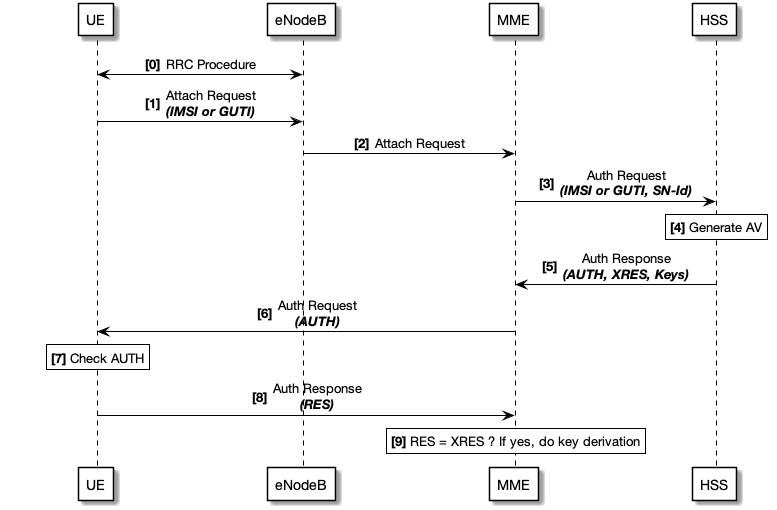
\includegraphics[width=\textwidth]{uml/4g-protocol_v1.png}
  \caption{Erfolgreiche Authentifikation}
  \label{fig:protocol_v1}
\end{figure} %A Comparative Introduction of 4G and 5G Authentication

\begin{enumerate}
\setcounter{enumi}{-1}
%0
\item Bevor das 4G EPS-AKA Protokoll mit \textit{Schritt 1} starten kann muss die \gls{rrc} Prozedur zwischen dem \gls{ue} und der \gls{enodeb} erfolgreich abgeschlossen sein.

%1
\item In Schritt 1 schickt das \gls{ue} den \textit{Attach Request} an den \gls{enodeb} und beginnt somit das 4G EPS-AKA Protokoll.
Die Nachricht enthält entweder die \gls{imsi} oder den \gls{guti} und wird durch das erfolgreiche abschließen der \gls{rrc} Prozedur ausgelöst.

%2
\item In Schritt 2 wird der \textit{Attach Request} aus \textit{Schritt 1} von der \gls{enodeb} an die \gls{mme} weitergesendet.

%3
\item In Schritt 3 sendet die \gls{mme} eine \textit{Auth Request} Nachricht an den \gls{hss}.
Sie enthält entweder die \gls{imsi} oder den \gls{guti}, den die \gls{mme} in \textit{Schritt 2} von der \gls{enodeb} in der \textit{Attach Request} Nachricht erhalten hat und zusätzlich noch die \gls{sn-id} des \textit{Serving Network}s zu dem die \gls{mme} gehört.

%4
\item In Schritt 4 wird aus dem geheimen Schlüssel \textit{K}, den sowohl der \gls{hss} wie auch das \gls{ue} kennen, der \gls{av} generiert.
Er beinhaltet unteranderem die \gls{xres}, die später mit der Antwort des \gls{ue}, \gls{res}, verglichen werden soll, den \gls{auth}, den das \gls{ue} für die Berechnung der \gls{res} benötigt und kryptographischen Schlüssel die im weiteren Verlauf benötigt werden.

%5
\item In Schritt 5 wird der in \textit{Schritt 4} generierte \gls{av} mit der \textit{Auth Response} Nachricht an die \gls{mme} gesendet.

%6
\item In Schritt 6 sendet die \gls{mme} einen \textit{Auth Request} direkt an das \gls{ue}.
Er enthält den \gls{auth}, den das \gls{ue} zur Berechnung der \gls{res} benötigt.

%7
\item Nachdem das \gls{ue} den \gls{auth} Parameter aus \textit{Schritt 6} erhalten hat wird er in Schritt 7 überprüft und daraus die \gls{res} berechnet.

%8
\item In Schritt 8 wird die \gls{res}, die in \textit{Schritt 7} berechnet wurde in einer \textit{Auth Response} Nachricht an die \gls{mme} gesendet.

%9
\item Nach Erhalt der \textit{Auth Response} Nachricht wird in Schritt 9 überprüft ob die \gls{res}, die die \gls{mme} in \textit{Schritt 8} erhalten hat, mit der \gls{xres}, die die \gls{mme} in \textit{Schritt 5} erhalten hat, übereinstimmt.
Ist dies der Fall, so wird aus den kryptographischen Schlüsseln, die die \gls{mme} ebenfalls in \textit{Schritt 5} erhalten hat, unteranderem der \gls{k-asme} der \gls{asme} berechnet, der beispielsweise für die Berechnung weiterer Schlüssel nach der erfolgreichen Authentifizierung benötigt wird.%3GPP TS 33.401 Page 19
\end{enumerate}


\section{Unterschiede von 4G EPS-AKA und 5G-AKA}

Das 4G-EPS-AKA Protokoll und das 5G-AKA Protokoll unterscheiden sich in folgenden Aspekten: %A Comparative Introduction of 4G and 5G Authentication

\begin{itemize}
%User Equipment
\item Das \gls{ue} hat sowohl bei 4G-EPS-AKA, wie auch bei 5G-AKA den gleichen Namen und ahnliche Aufgaben.
In beiden Protokollen beginnt bei dem \gls{ue} die Authentifizierung und ist der symmetrischen Langzeitschlüssel \gls{k} gespeichert.

%Serving Network
\item Das \textit{Serving Network} besteht im 4G EPS-AKA Protokoll aus der \gls{mme}. 
Die \gls{enodeb} kann auch als Teil des \textit{Serving Network}s gesehen werden.
Im 5G-AKA Protokoll hingegen besteht das \textit{Serving Network} nur aus der \gls{seaf}.

%Home Network
\item Im 4G EPS-AKA Protokoll besteht das \textit{Home Network} nur aus dem \gls{hss}.
Im 5G-AKA Protokoll hingegen gesteht das \textit{Home Network} aus der \gls{ausf} und aus dem \gls{udm}/\gls{arpf}/\gls{sidf}.

%Trust Model
\item Sowohl im 4G EPS-AKA wie auch im 5G-AKA Protokoll wird für die Authentifizierung der symmetrischer Langzeitschlüssel \gls{k} benötigt.
Er ist beim 4G EPS-AKA Protokoll im \gls{ue} und im \gls{hss} gespeichert.
Beim 5G-AKA Protokoll ist \gls{k} im \gls{ue} und im \gls{udm}/\gls{arpf} gespeichert.

%UE Identity
\item Jedes \gls{ue} hat eine Zeichenfolge, die es eindeutig identifiziert.
Diese ist jedoch bei den beiden Protokollen unterschiedlich.

Beim 4G EPS-AKA Protokoll kann bei der Kommunikation zwischen \gls{ue} und \textit{Serving Network} die \gls{imsi} oder der \gls{guti} und bei der Kommunikation zwischen \textit{Serving Network} und \textit{Home Network} nur die \gls{imsi} verwendet werden um das \gls{ue} eindeutig zu identifizieren.
Beim 5G-AKA Protokoll hingegen kann bei der Kommunikation zwischen \gls{ue} und \textit{Serving Network} der \gls{suci} oder der \gls{5g-guti} und bei der Kommunikation zwischen \textit{Serving Network} und \textit{Home Network} der \gls{suci} oder der \gls{supi} verwendet werden um das \gls{ue} eindeutig zu identifizieren.

Beim 5G-AKA Protokoll wird zwischen \gls{ue} und \textit{Serving Network} die Identität des \gls{ue} nur verschlüsselt, in Form des \gls{suci} oder des \gls{5g-guti} versendet. Beim 4G EPS-AKA Protokoll hingegen wird auch die unverschlüsselte \gls{imsi} zwischen \gls{ue} und \textit{Serving Network} versendet.

%SN Identity
\item Auch das \textit{Serving Network} kann eindeutig identifiziert werden.
Beim 4G EPS-AKA Protokoll wird das \textit{Serving Network} durch die \gls{sn-id} identifiziert.
Beim 5G-AKA Protokoll hingegen wird das \textit{Serving Network} durch den \gls{sn-name} identifiziert.

Die \gls{sn-id} und der \gls{sn-name} unterscheiden sich jedoch nur dadurch dass dem \gls{sn-name} zusätzlich noch ''5G:'' vorangestellt wurde.

%Authentication of UE decided by
\item Die Entscheidung ob die Authentifizierung erfolgreich war wird bei beiden Protokollen unterschiedlich gehandhabt.

Beim 4G EPS-AKA Protokoll entscheidet nur die \gls{mme}, die Teil des \textit{Serving Network}s ist, ob eine Authentifizierung erfolgreich war.
Die Entscheidung wird somit nur innerhalb des \textit{Serving Network}s getroffen.
Das \textit{Home Network} ist nicht an der Entscheidung beteiligt und wird auch nicht über den Ausgang der Authentifizierung informiert.

Beim 5G-AKA Protokoll hingegen entscheiden sowohl die \gls{seaf}, die Teil des \textit{Serving Network}s ist, wie auch die \gls{ausf}, die Teil des \textit{Home Network}s ist, ob die Authentifizierung erfolgreich war.
Die Entscheidung wird somit sowohl vom innerhalb des \textit{Serving Network}s, wie auch innerhalb des \textit{Home Network}s getroffen.
Des Weiteren benachrichtigt die \gls{ausf} auch das \gls{udm} über den Ausgang der Authentifizierung.
\end{itemize}
\chapter{Beschreibung einer Sicherheitsl\"ucke}
\label{chap:4}

Noch bevor eine endgültige Fassung des 5G-AKA Protokolls feststand haben sich einige Forscher bereits mit unterschiedlichen Sicherheitsaspekten des Protokolls auseinandergesetzt und teilweise sogar mögliche Sicherheitslücken entdeckt.
\textit{Martin Dehnel-Wild} und \textit{Cas Cremers} haben in \textit{Security vulnerability in 5G-AKA draft} solch eine Sicherheitslücke und dessen Auswirkungen, sowie mögliche Lösungsvorschläge vorgestellt. %Security vulnerability in 5G-AKA draft
Diese werden in diesem Kapitel vorgestellt.
Ihre Befunde beziehen sich auf die Spezifikation TS 33.501 V0.7.0 des 3GPP. %3GPP TS 33.501 V0.7.0
Mittlerweile hat das 3GPP bereits neuere Versionen der Spezifikation veröffentlicht, darunter auch die Version V15.34.1, auf der die Beschreibung aus \cref{chap:2} beruht. %3GPP TS 33.501 V15.34.1
Zur Verbesserung der Übersichtlichkeit wird daher im weiteren Verlauf die Sicherheitslücke im Kontext der Spezifikation TS 33.501 V15.34.1 beschrieben.


\section{Beschreibung der Sicherheitslücke}

\begin{figure}[H]
  \centering
  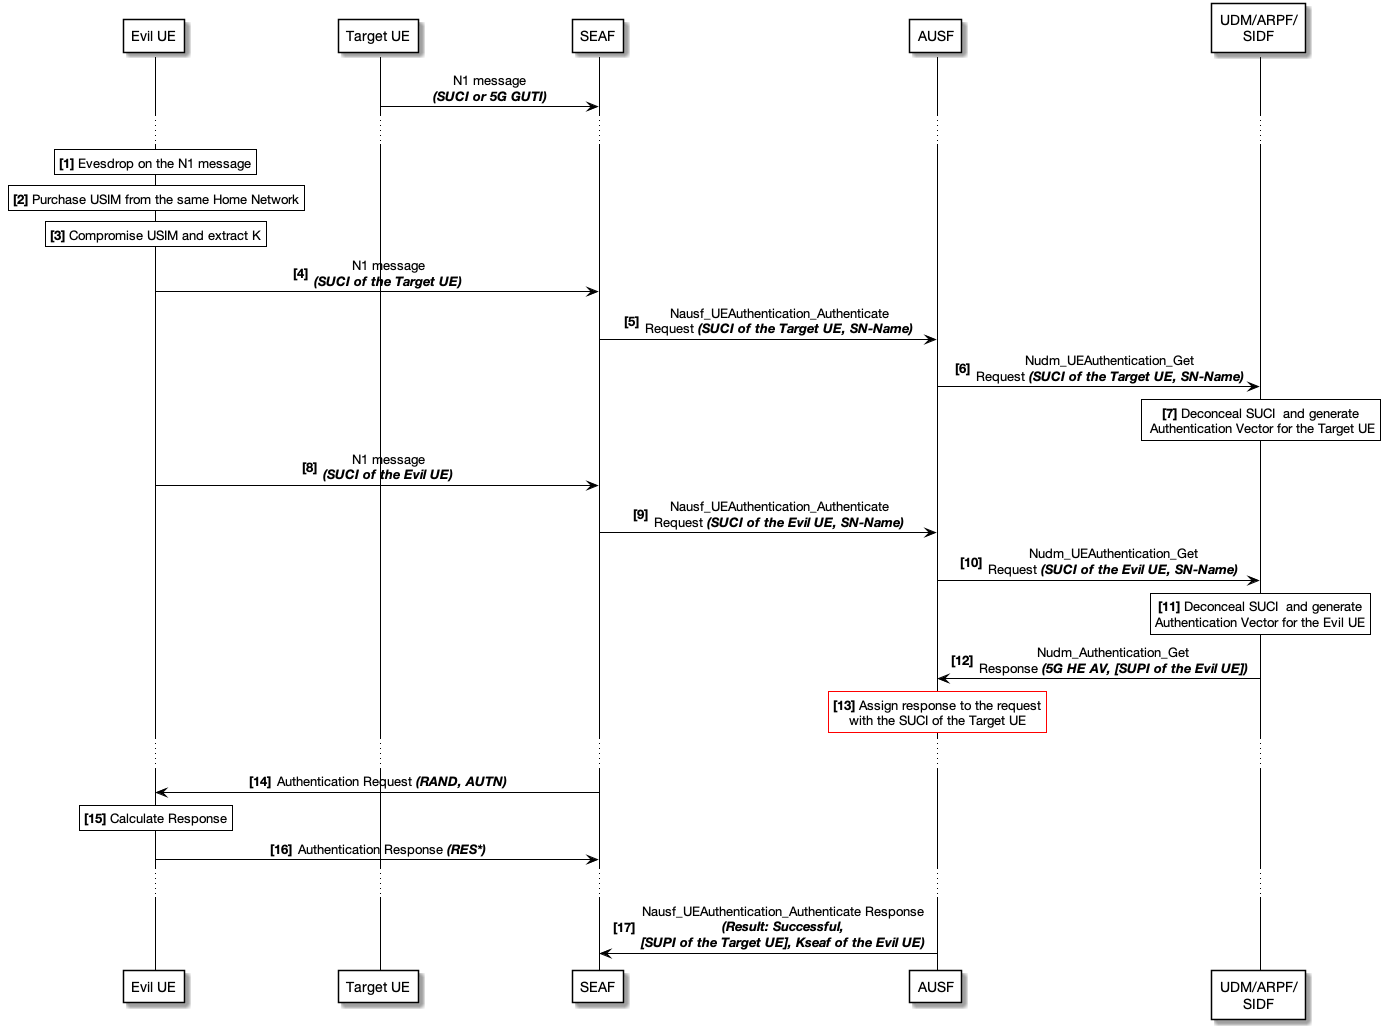
\includegraphics[width=\textwidth]{uml/vulnerability_v1.png}
  \caption{Beschreibung der Sicherheitslücke}
  \label{fig:vulnerability_v1}
\end{figure}

Die in dem \textit{Security vulnerability in 5G-AKA draft} vorgestellte Sicherheitslücke ermöglicht es einem Angreifer sich als ein anderer Benutzer auszugeben. %Security vulnerability in 5G-AKA draft
Zur Vereinfachung wird hier davon ausgegangen, dass das \gls{udm}/\gls{arpf}/\gls{sidf} immer das 5G-AKA Protokoll auswählt und nicht das EAP-AKA' Protokoll.
Hierbei handelt es sich um eine \textit{Race Condition}.
Der Angriff funktioniert also nicht in allen Versuchen.
Bevor er jedoch ausgeführt werden kann müssen einige Vorbereitungen getroffen werden.

\subsection{Vorbereitungen}

\begin{enumerate}
%1
\item Der Angreifer muss an den \gls{suci} des Benutzers kommen für den er sich ausgeben möchte.
Dafür muss er die \textit{N1 message} des Benutzers mithören und aufzeichnen.

%2
\item Hat der Angreifer die \textit{N1 message} des Benutzers aufgezeichnet, dann bringt er in Erfahrung zu welchem \textit{Home Network} der \gls{suci} gehört und kauft sich ein legitimes \gls{usim} des selben \textit{Home Network}s.

%3
\item Ist der Angreifer im Besitz des legitimen \gls{usim} so kompromittiert er dieses und extrahiert daraus den Langzeitschlüssel \gls{k}.

\end{enumerate}

\subsection{Der Hauptteil des Angriffs}

\begin{enumerate}
\setcounter{enumi}{3}

%4
\item Der Angreifer sendet nun eine \textit{N1 message} an die \gls{seaf} und initiiert somit eine neue Authentifikation.
Diese Nachricht enthält den \gls{suci} des Benutzers, den der Angreifer in \textit{Schritt 1} abgehört hat.

%5
\item Der \gls{suci} des abgehörten Benutzers wird von der \gls{seaf} an die \gls{ausf} weitergeleitet.

%6
\item Das \gls{udm} erhält den \gls{suci} des abgehörten Benutzers und beginnt die erhaltene Nachricht zu verarbeiten.

%7
\item Das \gls{udm} berechnet den \gls{supi} des abgehörten Benutzers aus dem \gls{suci} den es in \textit{Schritt 6} erhalten hat und generiert einen Authentifikations-Vektor für den \gls{suci} des abgehörten Benutzers.

%8
\item Direkt nach dem versenden der Nachricht aus \textit{Schritt 4} sendet der Angreifer erneut eine \textit{N1 message} jedoch dieses mal mit dem \gls{suci} des \gls{usim}s das er in \textit{Schritt 2} gekauft hat.

%9
\item Auch der \gls{suci} des Angreifers wird von der \gls{seaf} an die \gls{ausf} weitergeleitet.

%10
\item Das \gls{udm} erhält den \gls{suci} des Angreifers kurz nachdem es den \gls{suci} des abgehörten Benutzers erhalten hat.

%11
\item Das \gls{udm} berechnet den \gls{supi} des Angreifers aus dem \gls{suci}, den es in \textit{Schritt 9} erhalten hat und generiert den Authentifikations-Vektor  für den \gls{suci} des Angreifers.

%12
\item Das \gls{udm} hat in \textit{Schritt 7 \& 11} erst den \gls{suci} des abgehörten Benutzers und dann den \gls{suci} des Angreifers erhalten.
Nun sendet es aber erst den Authentifikations-Vektor für den \gls{suci} des Angreifers an die \gls{ausf} zurück.
Das \gls{udm} sendet also die Antworten auf die erhaltenen Nachrichten nicht in der gleichen Reihenfolge zurück in der es die \gls{suci}s erhalten hat.

In diesem Schritt (Schritt 12) wird in der hier beschriebenen Version(V15.34.1) zusätzlich zu dem \gls{5g-he-av} auch unter bestimmten Umständen der \gls{supi} mitgesendet.
Dies ist bei der Version(V0.7.0), auf der in dem \textit{Security vulnerability in 5G-AKA draft} eingegangen wird, nicht der Fall.

%13
\item Die \gls{ausf} erhält nun zuerst die Antwort auf die Nachricht aus \textit{Schritt 11}.
Da die Antwort des \gls{udm} nicht den \gls{suci} enthält kann die \gls{ausf} nicht überprüfen zu welchem \gls{suci} die Antwort gehört und nimmt daher fälschlicherweise an, dass die erhaltene Antwort zur Nachricht aus \textit{Schritt 6} gehört.

%14
\item In Schritt 14 erhält der Angreifer von der \gls{seaf} den Authentication Request.
Diese Nachricht enthält nun \gls{rand} und \gls{autn} die das \gls{udm} für den \gls{suci} des Angreifers, die \gls{seaf} jedoch nimmt an, das \gls{rand} und \gls{autn} für die Authentifizierung des abgehörten Benutzers bestimmt sind.

%15
\item Der Angreifer kann nun \gls{res*} aus \gls{rand} und \gls{autn} berechnen, da er in \textit{Schritt 3} den dafür benötigten Langzeitschlüssel \gls{k} erhalten hat.

%16
\item Der Angreifer sendet nun die in \textit{Schritt 15} berechnete \gls{res*} an die \gls{seaf}.

%17
\item Die \gls{seaf} und die \gls{ausf} überprüfen nun die \gls{res*} aus \textit{Schritt 16} und akzeptieren sie schließlich.
Das 5G-AKA Protokoll wurde also erfolgreich ausgeführt.
Jedoch nehmen \gls{seaf} und \gls{ausf} an, dass sich der abgehörte Benutzer erfolgreich authentifiziert hat und nicht der Angreifer.
Der Angreifer kann sich nun also dem \gls{seaf} gegenüber als den abgehörten Benutzer ausgeben.

Auch in diesem Schritt (Schritt 16) wird in der hier beschriebenen Version(V15.34.1) unter bestimmten Umständen der \gls{supi} mitgesendet nachdem er in \textit{Schritt 12} zwischengespeichert wurde.
Dies ist bei der Version(V0.7.0), auf der in dem \textit{Security vulnerability in 5G-AKA draft} eingegangen wird, nicht der Fall.


\end{enumerate}


\section{Verletzte Eigenschaft}

Nachdem der Angriff erfolgreich ausgeführt wurde sich die \gls{seaf}, die \gls{ausf} und der Angreifer im Besitz des \textit{''Anchor Key''}s \gls{k-seaf} und haben sich auf diesen geeinigt.
Des Weiteren sind glauben \gls{seaf} und die \gls{ausf}, dass der \gls{k-seaf} nur im Besitz des angehörten Benutzers und nicht im Besitz des Angreifers ist.

Es wird also die Eigenschaft verletzt, dass der \textit{''Anchor Key''} \gls{k-seaf} geheim seien soll.

Ein Angreifer kann somit, sofern er im Besitz eines beliebigen validen Langzeitschlüssels \gls{k} ist, sich als jeden anderen Benutzer ausgeben, der bei dem gleichen Provider eine \gls{usim} gekauft hat und dessen \gls{suci} dem Angreifer bekannt ist.


\section{Auswirkungen der Sicherheitslücke}

Diese Sicherheitslücke erlaubt es einem Angreifer sich als einen anderen Benutzer auszugeben.
Der Angriff kann unabhängig von der beim \gls{suci} verwendeten \textit{Protection Scheme} erfolgreich ausgeführt werden, es ist also nicht notwendig dass für die Verschlüsselung des \gls{suci} der \textit{Null Scheme} verwendet wurde.
Da der Angriff auf einer \textit{Race Condition} beruht kann nicht garantiert werden, dass er bei jedem Durchlauf erfolgreich durchgeführt wird.

Dieser Angriff erlaubt es nicht die Nachrichten zwischen einem abgehörten Benutzer und der \gls{seaf} zu entschlüsseln.

Ein Angreifer könnte sich jedoch als einen anderen Benutzer ausgeben und auf seinen Kosten Dienstleistungen des Providers in Anspruch nehmen.

Durch die Implementierung und andere technische Maßnahmen kann eine erfolgreiche Durchführung des Angriffs verhindert werden und somit verhindert werden das sich ein Angreifer als einen anderen Benutzer ausgibt.

In der hier beschriebenen Version(V15.34.1) wird in \textit{Schritt 7 \& 17} aus \cref{fig:protocol_v1} unter bestimmten Umständen auch der \gls{supi} mitgesendet.
Dies ist in der im \textit{Security vulnerability in 5G-AKA draft} betrachteten Version(V0.7.0) nicht der Fall und könnte die Funktionalität der Sicherheitslücke beeinträchtigen.


\section{Beschriebene Lösungsvorschläge}

\textit{Martin Dehnel-Wild} und \textit{Cas Cremers} haben in dem \textit{Security vulnerability in 5G-AKA draft} verschiedene Lösungsvorschläge beschrieben.

In dem ersten Lösungsansatz wird vorgeschlagen, dass in der \textit{Nudm\_Authentication\_Get Response} Nachricht aus \textit{Schritt 7} in \cref{fig:protocol_v1} zusätzlich \gls{suci} \& \gls{supi} und dass in der \textit{Nausf\_UEAuthentication\_Authenticate Response} Nachricht aus \textit{Schritt 10} aus \cref{fig:protocol_v1} zusätzlich der \gls{suci} mitgesendet wird.
Dies ermöglicht es der \gls{ausf} und der \gls{seaf} die erhaltenen Nachrichten eindeutig zuzuordnen und somit einen erfolgreichen Angriff zu verhindern.

Ein anderer Lösungsansatz schlägt vor, dass die Nachrichten zwischen der \gls{ausf} und der \gls{arpf} eine eindeutige Zufallszahl enthalten und somit klar zugeordnet werden können.







\chapter{Implementierung der Sicherheitsl\"ucke}
\label{chap:5}

Die in \cref{chap:4} beschriebene Sicherheitslücke und das 5G-AKA Protokoll wurde nun implementiert.
Die Implementierung ist dieser Arbeit beigefügt und kann auch auf Github unter folgendem Link eingesehen werden: \url{}//TODO
In diesem Kapitel wird sich auf den Commit \#ID gezogen.//TODO

Es wurde das 5G-AKA Protokoll aus der Spezifikation TS 33.501 des 3GPP mit der Version V15.34.1 implementiert.
Die Sicherheitslücke wurde darauf aufbauend implementiert.


\section{Ausführen des Programms}
Zum Ausführen des Programms wurde ein \textit{Gradle} Build Script bereitgestellt.
Es wird daher empfohlen die neueste Java und Gradle Version auf einem Linux Betriebssystem installiert zu haben.

Um das Programm auszuführen muss der Befehl \lstinline{gradle run} in eine Konsole eingegeben werden.
Dafür sollte man sich in dem Ordner befinden, in dem sich auch die build.gradle Datei befindet.

Alternativ kann auch der Gradle Wrapper ausgeführt werden.
Dafür muss auf Linux oder macOS der Befehl \lstinline{./gradlew run} und auf Windows der Befehl \lstinline{gradlew.bat run} ausgeführt werden.
Auch hier sollte man sich in dem Ordner befinden, in dem sich auch die build.gradle Datei befindet.

\subsection{Einstellungen}

Das Programm erlaubt es Einstellungen anzupassen, die das Verhalten des Programms beeinflussen.
Diese Einstellungen sind in der \lstinline{Implementation.App} Klasse zu finden und lassen sich folgendermaßen beschreiben:

\subsubsection{RUN\_MODE}
Der \textit{RUN\_MODE} beschreibt ob das Protokoll oder die Sicherheitslücke simuliert werden soll.
Er kann die Werte \lstinline{RunMode.Protocol} und \lstinline{RunMode.Vulnerability} annehmen.

Wird der \textit{RUN\_MODE} auf den Wert \lstinline{RunMode.Protocol} gesetzt, dann wird ein erfolgreicher normaler Durchlauf des Protokolls simuliert. 
Nach dem Durchlauf des Protokolls wird ausgegeben ob der Durchlauf erfolgreich war.

Wird der \textit{RUN\_MODE} auf den Wert \lstinline{RunMode.Vulnerability} gesetzt, dann wird der Angriff, wie er in \cref{chap:4} beschrieben ist, simuliert.
Nach dem Durchlauf wird ausgegeben ob Authentifizierung und Angriff erfolgreich waren.
Der Angriff kann nur erfolgreich sein wenn der Langzeitschlüssel \gls{k-seaf} bei dem \gls{ue} und der \gls{seaf} Entitäten gleich ist.
Mit der \textit{DETAILED\_AUTH\_INFO} Einstellung lassen sich die Langzeitschüssel auf der Konsole ausgeben.
Da der Angriff auf einer \textit{Race Condition} beruht ist auch das Fehlschlagen des simulierten Angriffs zu erwarten.

\subsubsection{LOG\_MESSAGES}

Mit \textit{LOG\_MESSAGES} lässt sich einstellen ob die von Entitäten empfangenen Nachrichten auf der Konsole ausgegeben werden sollen.
Es können die Werte \lstinline{true} und \lstinline{false} angegeben werden.

Wird \textit{LOG\_MESSAGES} auf \lstinline{true} gesetzt, dann werden auf der Konsole alle Nachrichten ausgeben, die von einer der Entitäten empfangen wurden.
Die Ausgabe auf der Konsole hat das Format: \textit{SENDER -> EMPFÄNGER : NACHRICHT}

Wird \textit{LOG\_MESSAGES} auf \lstinline{false} gesetzt, dann werden die empfangenen Nachrichten nicht auf der Konsole ausgegeben.

\subsubsection{DETAILED\_AUTH\_INFO}

Mit \textit{DETAILED\_AUTH\_INFO} lässt sich einstellen ob detaillierte Informationen auf der Konsole ausgegeben werden sollen.
Es können die Werte \lstinline{true} und \lstinline{false} angegeben werden.

Wird \textit{DETAILED\_AUTH\_INFO} auf \lstinline{true} gesetzt, dann werden detaillierte Informationen zur Authentifizierung auf der Konsole ausgegeben.
Dies beinhaltet Informationen darüber ob die Authentifizierung von der \gls{seaf}, der \gls{ausf} und dem \gls{udm} als erfolgreich angesehen wird, wie es in \textit{Schritt 14 \& 16} von \cref{fig:protocol_v1} beschrieben ist.
Des Weiteren wird der Langzeitschlüssel \gls{k-seaf} der im \gls{ue} und in der \gls{seaf} gespeichert ist ausgegeben.

Wird \textit{DETAILED\_AUTH\_INFO} auf \lstinline{false} gesetzt, dann werden keine detaillierten Informationen zur Authentifizierung auf der Konsole ausgegeben.


\section{Beschreibung des Aufbaus}
Für die Implementierung wurde die Programmiersprache Java gewählt.

Der Einstiegspunkt des Programms ist die \lstinline{Implementation.App} Klasse. Von dort lässt sich das Programm mit der \lstinline{main} Methode aufrufen.

In dem \lstinline{Implementation.structure} Package wird die grundlegende Struktur für Entitäten und Nachrichten definiert.
Alle Entitäten haben die \lstinline{Implementation.structure.Entity} Klasse als Superklasse und alle Nachrichten haben das \lstinline{Implementation.structure.Message} Interface implementiert.

Das \lstinline{Implementation.helper} Package beinhaltet Helferklassen.
Diese Helferklassen werden verwendet um die Übersichtlichkeit in den anderen Packages zu verbessern.
Sie beinhalten nur statische Methoden.

In dem \lstinline{Implementation.protocol} Package ist die tatsächliche Implementierung des Protokolls zu finden.
Es ist unterteilt in die Packages \lstinline{Implementation.protocol.additional}, \lstinline{Implementation.protocol.data}, \lstinline{Implementation.protocol.entities} und \lstinline{Implementation.protocol.messages}.

Das \lstinline{Implementation.protocol.additional} Package beinhaltet hauptsächlich Klassen die kryptographischen Berechnungen ausführen, wie die \gls{kdf}.
Alle Klassen in diesem Package beinhalten nur statische Methoden.

Das \lstinline{Implementation.protocol.data} Package beinhaltet Klassen, die mehrere verschiedene Parameter in sich zusammenfassen, wie z.B. der \gls{5g-he-av}.

In dem \lstinline{Implementation.protocol.entities} Package ist die Implementierung der vier Entitäten \gls{ue}, \gls{seaf}, \gls{ausf} und \gls{udm} zu finden, so wie eine \lstinline{EvilUE} Klasse, die den Angreifer darstellen soll.
In diesen Klassen ist das Versenden und Antworten auf Nachrichten implementiert.
Dies geschieht über die \lstinline{Implementation.structure.Entity} Superklasse.

In dem \lstinline{Implementation.protocol.messages} Package sind alle Nachrichten zu finden, die die Entitäten untereinander verschicken.
Jede Nachricht hat eine eigene Klasse, die das \lstinline{Implementation.structure.Message} Interface implementiert.


\subsection{Implementierung der Race Condition}
Um die \textit{Race Condition} zu realisieren muss sichergestellt werden dass versendete Nachrichten sich überholen können.
Dies wurde mit Hilfe von \textit{Threads} implementiert.
Dafür wurden in der \lstinline{Implementation.structure.Entity} Klasse die \lstinline{sendMessage} Methode erstellt.
Da die \lstinline{Implementation.structure.Entity} Klasse die Superklasse von allen Entitäten ist wird in den Entitäten die \lstinline{sendMessage} der \lstinline{Implementation.structure.Entity} Klasse verwendet um Nachrichten zu versenden.

Führt eine Entität die \lstinline{sendMessage} Methode aus, so wird ein neuer Thread erzeugt der die \lstinline{onReceiveMessage} Methode asynchron auf der Entität ausführt, die die gesendete Nachricht erhalten soll.
Somit ist sichergestellt, dass eine \textit{Race Condition} möglich ist.


\subsection{Unterschiede zum Protokoll}
Ziel dieser Implementierung ist es die Praktikabilität der in \cref{chap:4} beschriebenen Sicherheitslücke herauszufinden.
In der Implementierung wurde daher einige Teile der Protokolls, die für die Sicherheitslücke nicht relevant sind, verändert oder weggelassen.
Nachfolgend ist eine Liste aller Abweichungen vom Protokoll aufgeführt.
Alle Abweichungen sind im Code mit dem Kommentar \lstinline{//MARK: Deviation #} versehen.
Das \lstinline{#} entspricht der Nummer der Abweichung.

\begin{enumerate}
%1
\item In der \lstinline{Implementation.protocol.additional.AVGenerator} Klasse wurde bei der Generierung der \gls{sqn} in der \lstinline{generateSQN} Methode von der Spezifikation abgewichen.
In der Spezifikation wurden Bedingungen, wie die \textit{Wrap around Protection}, für die Generierung der \gls{sqn} festgelegt.
In der Implementierung wurde jedoch die \gls{sqn} mit einem Zufallsgenerator generiert, der diese Bedingungen nicht erfüllt.

%2
\item In der \lstinline{Implementation.protocol.additional.KGF} Klasse wurde bei der \textit{Message authentication function} f1 von der Spezifikation abgewichen.
In der Spezifikation ist für die \lstinline{f1} Methode eine \textit{Message authentication function} gefordert.
In der Implementierung wurde hierfür jedoch die letzten 8 Bytes des \textit{HmacSHA256} verwendet.

%3
\item In der \lstinline{Implementation.protocol.additional.KGF} Klasse wurde bei der \textit{Message authentication function} f2 von der Spezifikation abgewichen.
In der Spezifikation ist für die \lstinline{f2} Methode eine \textit{Message authentication function} gefordert.
In der Implementierung wurde hierfür jedoch der \textit{HmacSHA256} verwendet.

%4
\item In der \lstinline{Implementation.protocol.additional.MAF} Klasse wurde bei der \textit{Key generation function} f3 von der Spezifikation abgewichen.
In der Spezifikation ist für die \lstinline{f3} Methode eine \textit{Key generating function} gefordert.
In der Implementierung wurde hierfür jedoch die letzten 16 Bytes des \textit{HmacSHA256} verwendet.

%5
\item In der \lstinline{Implementation.protocol.additional.MAF} Klasse wurde bei der \textit{Key generation function} f4 von der Spezifikation abgewichen.
In der Spezifikation ist für die \lstinline{f4} Methode eine \textit{Key generating function} gefordert.
In der Implementierung wurde hierfür, wie auch bei der Abweichung Nr. 4, die letzten 16 Bytes des \textit{HmacSHA256} verwendet.

%6
\item In der \lstinline{Implementation.protocol.additional.MAF} Klasse wurde bei der \textit{Key generation function} f5 von der Spezifikation abgewichen.
In der Spezifikation ist für die \lstinline{f5} Methode eine \textit{Key generating function} gefordert.
In der Implementierung wurde hierfür jedoch die letzten 6 Bytes des \textit{HmacSHA256} verwendet.

%7
\item In der \lstinline{Implementation.protocol.additional.SIDF} Klasse wurde bei der Entschlüsselung des \gls{suci} in den \gls{supi} von der Spezifikation abgewichen.
In der Spezifikation ist der \gls{suci} ein kompliziertes Bitfeld und bedarf somit einer umfangreichen Entschlüsselungsfunktion.
Die Implementierung der \lstinline{deconcealSUCI} Methode verwendet jedoch nur das \textit{RSA} Verfahren zum entschlüsseln.

%8
\item In der \lstinline{Implementation.protocol.additional.SIDF} Klasse wurde bei der Verschlüsselung des \gls{supi} in den \gls{suci} von der Spezifikation abgewichen.
In der Spezifikation ist der \gls{suci} ein kompliziertes Bitfeld. Dies muss eine Verschlüsselungsfunktion berücksichtigen.
Die Implementierung der \lstinline{deconcealSUCI} Methode verwendet jedoch nur das \textit{RSA} Verfahren zum verschlüsseln.
Daher entspricht der \gls{suci} in der Implementierung auch nur dem Ergebnis des \textit{RSA} Verfahrens und nicht dem Bitfeld das in der Spezifikation beschrieben wurde.

%9
\item Da in der Sicherheitslücke der \gls{5g-guti} nicht verwendet wird, wurde der \gls{5g-guti} nicht implementiert.

%10
\item In \textit{Schritt 3} der \cref{fig:protocol_v1} soll die \gls{ausf} einer \gls{seaf}, die den mitgesendeten \gls{sn-name} nicht verwenden darf, mit einer \textit{serving network not authorized} Nachricht antworten.
In der Implementierung sendet die \lstinline{Implementierung.protocol.entities.AUSF} Klasse diese Nachricht nicht.

%11
\item In \textit{Schritt 3} der \cref{fig:protocol_v1} soll die \gls{ausf} überprüfen ob eine \gls{seaf}, die eine Nachricht an die \gls{ausf} geschickt hat, den mitgesendeten \gls{sn-name} verwenden darf.
In der Implementierung tut dies die \lstinline{Implementation.protocol.entities.AUSF} Klasse nicht.

%12
\item In \textit{Schritt 17} der \cref{fig:protocol_v1} wird beschrieben, dass die \gls{ausf} der \gls{seaf} den \gls{supi} des Benutzer mitsendet, wenn die \gls{ausf} diesen in \textit{Schritt 7} erhalten hat.
Hat sie den \gls{supi} nicht in \textit{Schritt 7} erhalten, so wurde in \textit{Schritt 1} der \gls{5g-guti} an die \gls{seaf} gesendet.
Da jedoch bei dem implementierten Angriff nie der \gls{5g-guti} versendet wird, wurde in der \lstinline{Implementation.protocol.entities.SEAF} Klasse die Nachricht aus \textit{Schritt 17} nur mit mitgesendetem \gls{supi} behandelt.

%13
\item Erhält die \gls{seaf} eine \textit{Authentication Failure} Nachricht vom \gls{ue} so soll sie im Falle einer \textit{Synchronization failure} eine neue Authentifizierung initiieren können.
In der Implementierung wird in der \lstinline{Implemenation.protocol.entities.SEAF} Klasse jedoch nie eine neue Authentifizierung initiiert.

%14
\item In \textit{Schritt 14} der \cref{fig:protocol_v1} soll die \gls{seaf} bei einer zu spät oder nicht erhaltener Nachricht die Authentifizierung abbrechen.
In der Implementierung wird die erhaltene Nachricht jedoch immer akzeptiert.
Es gibt also keinen \textit{Timeout}.

%15
\item In \textit{Schritt 12} der \cref{fig:protocol_v1} wird überprüft ob der \gls{autn} angenommen werden kann.
In der Implementierung wurde in der \lstinline{Implementation.protocol.entities.UE} Klasse diese Überprüfung weggelassen.

%16
\item In \textit{Schritt 2*} der \cref{fig:protocol_mac_failure_v1} sendet das \gls{ue} eine \textit{Authentication Failure} Nachricht an die \gls{seaf}.
Diese Nachricht enthält auch einen CAUSE Wert, der den Grund des Fehlschlagens beschreibt.
In der Implementierung wird jedoch kein CAUSE Wert in der \textit{Authentication Failure} Nachricht mitgesendet.

%17
\item In \textit{Schritt 11} der \cref{fig:protocol_v1} sendet die \gls{seaf} in der \textit{Authentication Request} Nachricht zusätzlich noch den \gls{ng-ksi} und die \gls{abba} mit.
In der Implementierung werden diese Parameter jedoch nicht mitgesendet.

%18
\item In \textit{Schritt 15} der \cref{fig:protocol_v1} sendet die \gls{seaf} eine \textit{Nausf\_UEAuthentication\_Authenticate Request} Nachricht an die \gls{ausf}.
In der Implementierung wurde diese Nachricht in \textit{Nausf\_UEAuthentication\_Confirmation Request} umbenannt, da die Nachricht aus \textit{Schritt 2} sonst den gleichen Name hätte.

%19
\item In \textit{Schritt 17} der \cref{fig:protocol_v1} sendet die \gls{ausf} eine \textit{Nausf\_UEAuthentication\_Authenticate Response} Nachricht an die \gls{seaf}.
In der Implementierung wurde diese Nachricht in \textit{Nausf\_UEAuthentication\_Confirmation Response} umbenannt, da die Nachricht aus \textit{Schritt 10} sonst den gleichen Name hätte.

%20
\item In \textit{Schritt 7} der \cref{fig:protocol_v1} wird zusätzlich zum \gls{5g-he-av} der Hinweis mitgesendet, dass der \gls{5g-he-av} für das 5G-AKA Protokoll bestimmt ist.
In der Implementierung wurde dieser Hinweis weggelassen.

%21
\item Der \gls{supi} ist als ein Bitfeld spezifiziert, das aus mehreren Parametern besteht.
In der Implementierung ist der \gls{supi} jedoch nur eine zufällige Bitfolge.


\end{enumerate}


\section{Übersicht der Komponenten}


\chapter{Zusammenfassung und Ausblick}
\label{chap:6}

In dieser Arbeit wurde das 5G-AKA Protokoll erklärt und mit dem 4G EPS-AKA Protokoll verglichen.
Außerdem wurde eine Sicherheitslücke des 5G-AKA Protokolls erklärt und implementiert.

Das 5G-AKA Protokoll ist eines von zwei Protokollen des 5G-Standards das für den sicheren Austausch eines kryptographischen Schlüssels zuständig ist.
Es besteht aus den 4 Entitäten \gls{ue}, \gls{seaf}, \gls{ausf} und \gls{udm}.
Das \gls{ue} entspricht z.B. dem Smartphone eines Benutzers, die \gls{seaf} entspricht z.B. einem Funkmast mit dem sich das Smartphone des Benutzers verbindet und die \gls{ausf} und das \gls{udm} entsprechen z.B. dem Provider, von dem der Benutzer eine SIM-Karte gekauft hat.
Über diese vier Entitäten werden nun Nachrichten versendet, die das \gls{ue} authentifizieren und einen gemeinsamen Schlüssel austauschen.
War das 5G-AKA Protokoll erfolgreich, dann verfügen das \gls{ue} und die \gls{seaf} über einen \textit{Anchor Key}, genannt \gls{k-seaf}, der für die weitere Verschlüsselung verwendet wird.

Das 5G-AKA Protokoll hat einige Verbesserungen gegenüber dem 4G EPS-AKA Protokoll des 4G-Standards.
Jedoch wurde auch in dem 5G-AKA Protokoll eine Sicherheitslücke entdeckt.
In dieser Sicherheitslücke geht es darum, dass sich ein Angreifer als ein anderer Benutzer ausgeben kann.
Der Angreifer muss dafür den verschlüsselten Identifier des Benutzers, genannt \gls{suci}, abhören, sowie ein SIM-Karte bei dem Provider kaufen, bei dem auch der Benutzer seine SIM-Karte gekauft hat.
Der Angreifer hat nun die Möglichkeit sich als diesen Benutzer auszugeben.
Der Angriff beruht auf einer \textit{Race Condition}, ist also nicht immer erfolgreich.
Des Weiteren wurde der Angriff für eine ältere Version des 5G-AKA Protokolls gefunden.
Es kann also sein, dass dieser Angriff bis zur kommerziellen Verwendung des 5G-Standards nicht mehr möglich ist.


\section*{Ausblick}
Das 5G-AKA Protokoll befindet sich zurzeit noch in der Entwicklung und ist bisher nur in wenigen Städten verfügbar.
Während der Erstellung dieser Arbeit wurden auch bereits mehrere neue Versionen der Spezifikation des 5G-AKA Protokolls veröffentlicht.
Diese Entwicklung zeigt, dass sich das Protokoll bis zu seiner flächendeckenden Verwendung noch verändern und weiterentwickeln wird.
Daher ist es nahelegend, dass die hier vorgestellte Sicherheitslücke einen Benutzer möglicherweise nicht betreffen wird.


\printbibliography

Alle URLs wurden zuletzt am 17.\,03.\,2018 geprüft.

%\renewcommand{\appendixtocname}{Anhang}
%\renewcommand{\appendixname}{Anhang}
%\renewcommand{\appendixpagename}{Anhang}
\appendix
% !TeX root = main-german.tex
% !TeX spellcheck = de_DE
% !TeX encoding = utf8
% -*- coding:utf-8 mod:LaTeX -*-

%Die Angabe des schlauen Spruchs auf diesem Wege funtioniert nur,
%wenn keine Änderung des Kapitels mittels den in preambel/chapterheads.tex
%vorgeschlagenen Möglichkeiten durchgeführt wurde.
\setchapterpreamble[u]{%
  \dictum[Albert Einstein]{Probleme kann man niemals mit derselben Denkweise lösen, durch die sie entstanden sind.}
}
\chapter{LaTeX-Tipps}
\label{chap:latextipps}

In diesem Kapitel sollen allgemeine \LaTeX-Hinweise gegeben werden.

\section{Trennung von Absätzen}

Pro Satz eine neue Zeile.
Das ist wichtig, um sauber versionieren zu können.
In LaTeX werden Absätze durch eine Leerzeile getrennt.
Analogie zu Word: Bei Word werden neue Absätze durch einmal Eingabetaste gemacht.
Dies führt bei LaTeX jedoch nicht zu einem neuen Absatz, da LaTeX direkt aufeinanderfolgende Zeilen zu einer Zeile zusammenfügt.
Möchte man nun einen Absatz haben, muss man zweimal die Eingabetaste drücken.
Dies führt zu einer leeren Zeile.
In Word gibt es die Funktion Großschreibetaste und Eingabetaste gleichzeitig.
Wenn man dies drückt, wird einer harter Umbruch erzwungen.
Der Text fängt am Anfang der neuen Zeile an.
In LaTeX erreicht man dies durch Doppelbackslashes (\textbackslash\textbackslash) erzeugt.
Dies verwendet man quasi nie.

Folglich werden neue Abstäze insbesondere \emph{nicht} durch Doppelbackslashes erzeugt.
Beispielsweise begann der letzte Satz in einem neuen Absatz.
Eine ausführliche Motivation hierfür findet sich in \url{http://loopspace.mathforge.org/HowDidIDoThat/TeX/VCS/#section.3}.

Möchte man die Art des Absatzes ändern, so kann man die Dokumentklassenoption \texttt{parskip} verwenden.
Beispielsweise kann man mit \texttt{parskip=off} erreichen, dass statt eines freien Bereichs die erste Zeile des Absatzes eingezogen wird.

\section{File-Encoding und Unterstützung von Umlauten}
\label{sec:firstsectioninlatexhints}
Die Vorlage wurde 2010 auf UTF-8 umgestellt.
Alle neueren Editoren sollten damit keine Schwierigkeiten haben.

\section{Zitate}
Referenzen werden mittels \texttt{\textbackslash cite[key]} gesetzt.
Beispiel: \cite{WSPA} oder mit Autorenangabe: \citet{WSPA}.

Der folgende Satz demonstriert 
\begin{filecontents*}{\democodefile}
\begin{inparaenum}[1.]
  \item die Großschreibung von Autorennamen am Satzanfang,
  \item die richtige Zitation unter Verwendung von Autorennamen und der Referenz,
  \item dass die Autorennamen ein Hyperlink auf das Literaturverzeichnis sind sowie
  \item dass in dem Literaturverzeichnis der Namenspräfix \qq{van der} von \qq{Wil M.\,P.\ van der Aalst} steht.
\end{inparaenum}
\end{filecontents*}

\PrintDemo{style=parallel}

\Citet{RVvdA2016} präsentieren eine Studie über die Effektivität von Workflow-Management-Systemen.

Der folgende Satz demonstriert, dass man mittels \texttt{label} in einem Bibliopgrahie"=Eintrag den Textteil des generierten Labels überschreiben kann, aber das Jahr und die Eindeutigkeit noch von biber generiert wird.
Die Apache ODE Engine \cite{ApacheODE} ist eine Workflow-Maschine, die \BPEL-Prozesse zuverlässig ausführt.

Wörter am besten mittels \texttt{\textbackslash qq\{...\}} \qq{einschließen}, dann werden die richtigen Anführungszeichen verwendet.

Beim Erstellen der Bibtex-Datei wird empfohlen darauf zu achten, dass die DOI aufgeführt wird.

\section{Mathematische Formeln}
\label{sec:mf}
Mathematische Formeln kann man $so$ setzen. \texttt{symbols-a4.pdf} (zu finden auf \url{http://texdoc.net/pkg/symbols-a4}) enthält eine Liste der unter LaTeX direkt verfügbaren Symbole.
Beispielsweise $\mathbb{N}$ für die Menge der natürlichen Zahlen.
Für eine vollständige Dokumentation für mathematischen Formelsatz sollte die Dokumentation zu \texttt{amsmath}, \url{http://texdoc.net/pkg/amsmath} gelesen werden.

Folgende Gleichung erhält keine Nummer, da \texttt{\textbackslash equation*} verwendet wurde.
\begin{filecontents*}{\democodefile}
\begin{equation*}
  x = y
\end{equation*}
\end{filecontents*}

\PrintDemo{style=parallel}

Die Gleichung~\ref{eq:test} erhält eine Nummer:
\begin{filecontents*}{\democodefile}
\begin{equation}
  \label{eq:test}
  x = y
\end{equation}
\end{filecontents*}

\PrintDemo{style=parallel}

Die Vorlage bietet \verb+\abs+ an, damit die Absolutbetragsstriche richtig skalieren:
$\abs{X}$.

Eine ausführliche Anleitung zum Mathematikmodus von LaTeX findet sich in \url{http://www.ctan.org/tex-archive/help/Catalogue/entries/voss-mathmode.html}.

\section{Quellcode}
\Cref{lst:ListingANDlstlisting,helloworld} zeigen, wie man Programmlistings einbindet.
Mittels \texttt{\textbackslash lstinputlisting} kann man den Inhalt direkt aus Dateien lesen.

%Listing-Umgebung wurde durch \newfloat{Listing} definiert

\begin{Listing}
  \begin{lstlisting}[language=XML]
<listing name="second sample">
  <!-- comment -->
  <content>not interesting</content>
</listing>
\end{lstlisting}
  \caption{lstlisting in einer Listings-Umgebung, damit das Listing durch Balken abgetrennt ist}
  \label{lst:ListingANDlstlisting}
\end{Listing}


%TODO: Currently not shown in TOC
\lstinputlisting[language=C++,label=helloworld,caption={"`hello world"' in C++.},float]{code/helloworld.cpp}

Quellcode im \lstinline|<listing />| ist auch möglich.


\section{Pseudocode}
\Cref{alg:sample} zeigt einen Beispielalgorithmus.


\begin{Algorithmus} %Die Umgebung nur benutzen, wenn man den Algorithmus ähnlich wie Graphiken von TeX platzieren lassen möchte
  \caption{Sample algorithm}
  \label{alg:sample}
  %EN: This is an environment from the algorithmicx package
  \begin{algorithmic}
    \Procedure{Sample}{$a$,$v_e$}
      \State $\mathsf{parentHandled} \gets (a = \mathsf{process}) \lor \mathsf{visited}(a'), (a',c,a) \in \mathsf{HR}$
      \State \Comment $(a',c'a) \in \mathsf{HR}$ denotes that $a'$ is the parent of $a$
    \If{$\mathsf{parentHandled}\,\land(\mathcal{L}_\mathit{in}(a)=\emptyset\,\lor\,\forall l \in \mathcal{L}_\mathit{in}(a): \mathsf{visited}(l))$}
      \State $\mathsf{visited}(a) \gets \text{true}$
      \State $\mathsf{writes}_\circ(a,v_e) \gets
        \begin{cases}
          \mathsf{joinLinks}(a,v_e)                & \abs{\mathcal{L}_\mathit{in}(a)} > 0 \\
          \mathsf{writes}_\circ(p,v_e)
                                                   & \exists p: (p,c,a) \in \mathsf{HR}   \\
          (\emptyset, \emptyset, \emptyset, false) & \text{otherwise}
        \end{cases}
      $
    \If{$a\in\mathcal{A}_\mathit{basic}$}
      \State \Call{HandleBasicActivity}{$a$,$v_e$}
    \ElsIf{$a\in\mathcal{A}_\mathit{flow}$}
      \State \Call{HandleFlow}{$a$,$v_e$}
    \ElsIf{$a = \mathsf{process}$} \Comment Directly handle the contained activity
      \State \Call{HandleActivity}{$a'$,$v_e$}, $(a,\bot,a') \in \mathsf{HR}$
      \State $\mathsf{writes}_\bullet(a) \gets \mathsf{writes}_\bullet(a')$
    \EndIf
    \ForAll{$l \in \mathcal{L}_\mathit{out}(a)$}
      \State \Call{HandleLink}{$l$,$v_e$}
    \EndFor
    \EndIf
    \EndProcedure
  \end{algorithmic}
\end{Algorithmus}

\clearpage
Und wer einen Algorithmus schreiben möchte, der über mehrere Seiten geht, der kann das nur mit folgendem \textbf{üblen} Hack tun:

{
\begin{minipage}{\textwidth}
  \hrule height .8pt width\textwidth
  \vskip.3em%\vskip\abovecaptionskip\relax
  \stepcounter{Algorithmus}
  \addcontentsline{alg}{Algorithmus}{\protect\numberline{\theAlgorithmus}{\ignorespaces Description \relax}}
  \noindent\textbf{Algorithmus \theAlgorithmus} Description
  %\stepcounter{algorithm}
  %\addcontentsline{alg}{Algorithmus}{\thealgorithm{}\hskip0em Description}
  %\textbf{Algorithmus \thealgorithm} Description
  \vskip.3em%\vskip\belowcaptionskip\relax
  \hrule height .5pt width\textwidth
\end{minipage}
%without the following line, the text is nerer at the rule
\vskip-.3em
%
code goes here\\
test2\\
%
\vskip-.7em
\hrule height .5pt width\textwidth
}




\section{Abbildungen}

Die \cref{fig:chor1} und \ref{fig:chor2} sind für das Verständnis dieses Dokuments wichtig.
Im Anhang zeigt \vref{fig:AnhangsChor} erneut die komplette Choreographie.

%Die Parameter in eckigen Klammern sind optionale Parameter - z.B. [htb!]
%htb! bedeutet: "Liebes LaTeX, bitte platziere diese Abbildung zuerst hier ("_h_ere"). Falls das nicht funktioniert, dann bitte oben auf der Seite ("_t_op"). Und falls das nicht geht, bitte unten auf der Seite ("_b_ottom"). Und bitte, bitte bevorzuge hier und oben, auch wenn's net so optimal aussieht ("!")
%Diese sollten nach Möglichkeit NICHT verwendet werden. LaTeX's Algorithmus für das Platzieren der Gleitumgebung ist schon sehr gut!

\begin{figure}
  \centering
  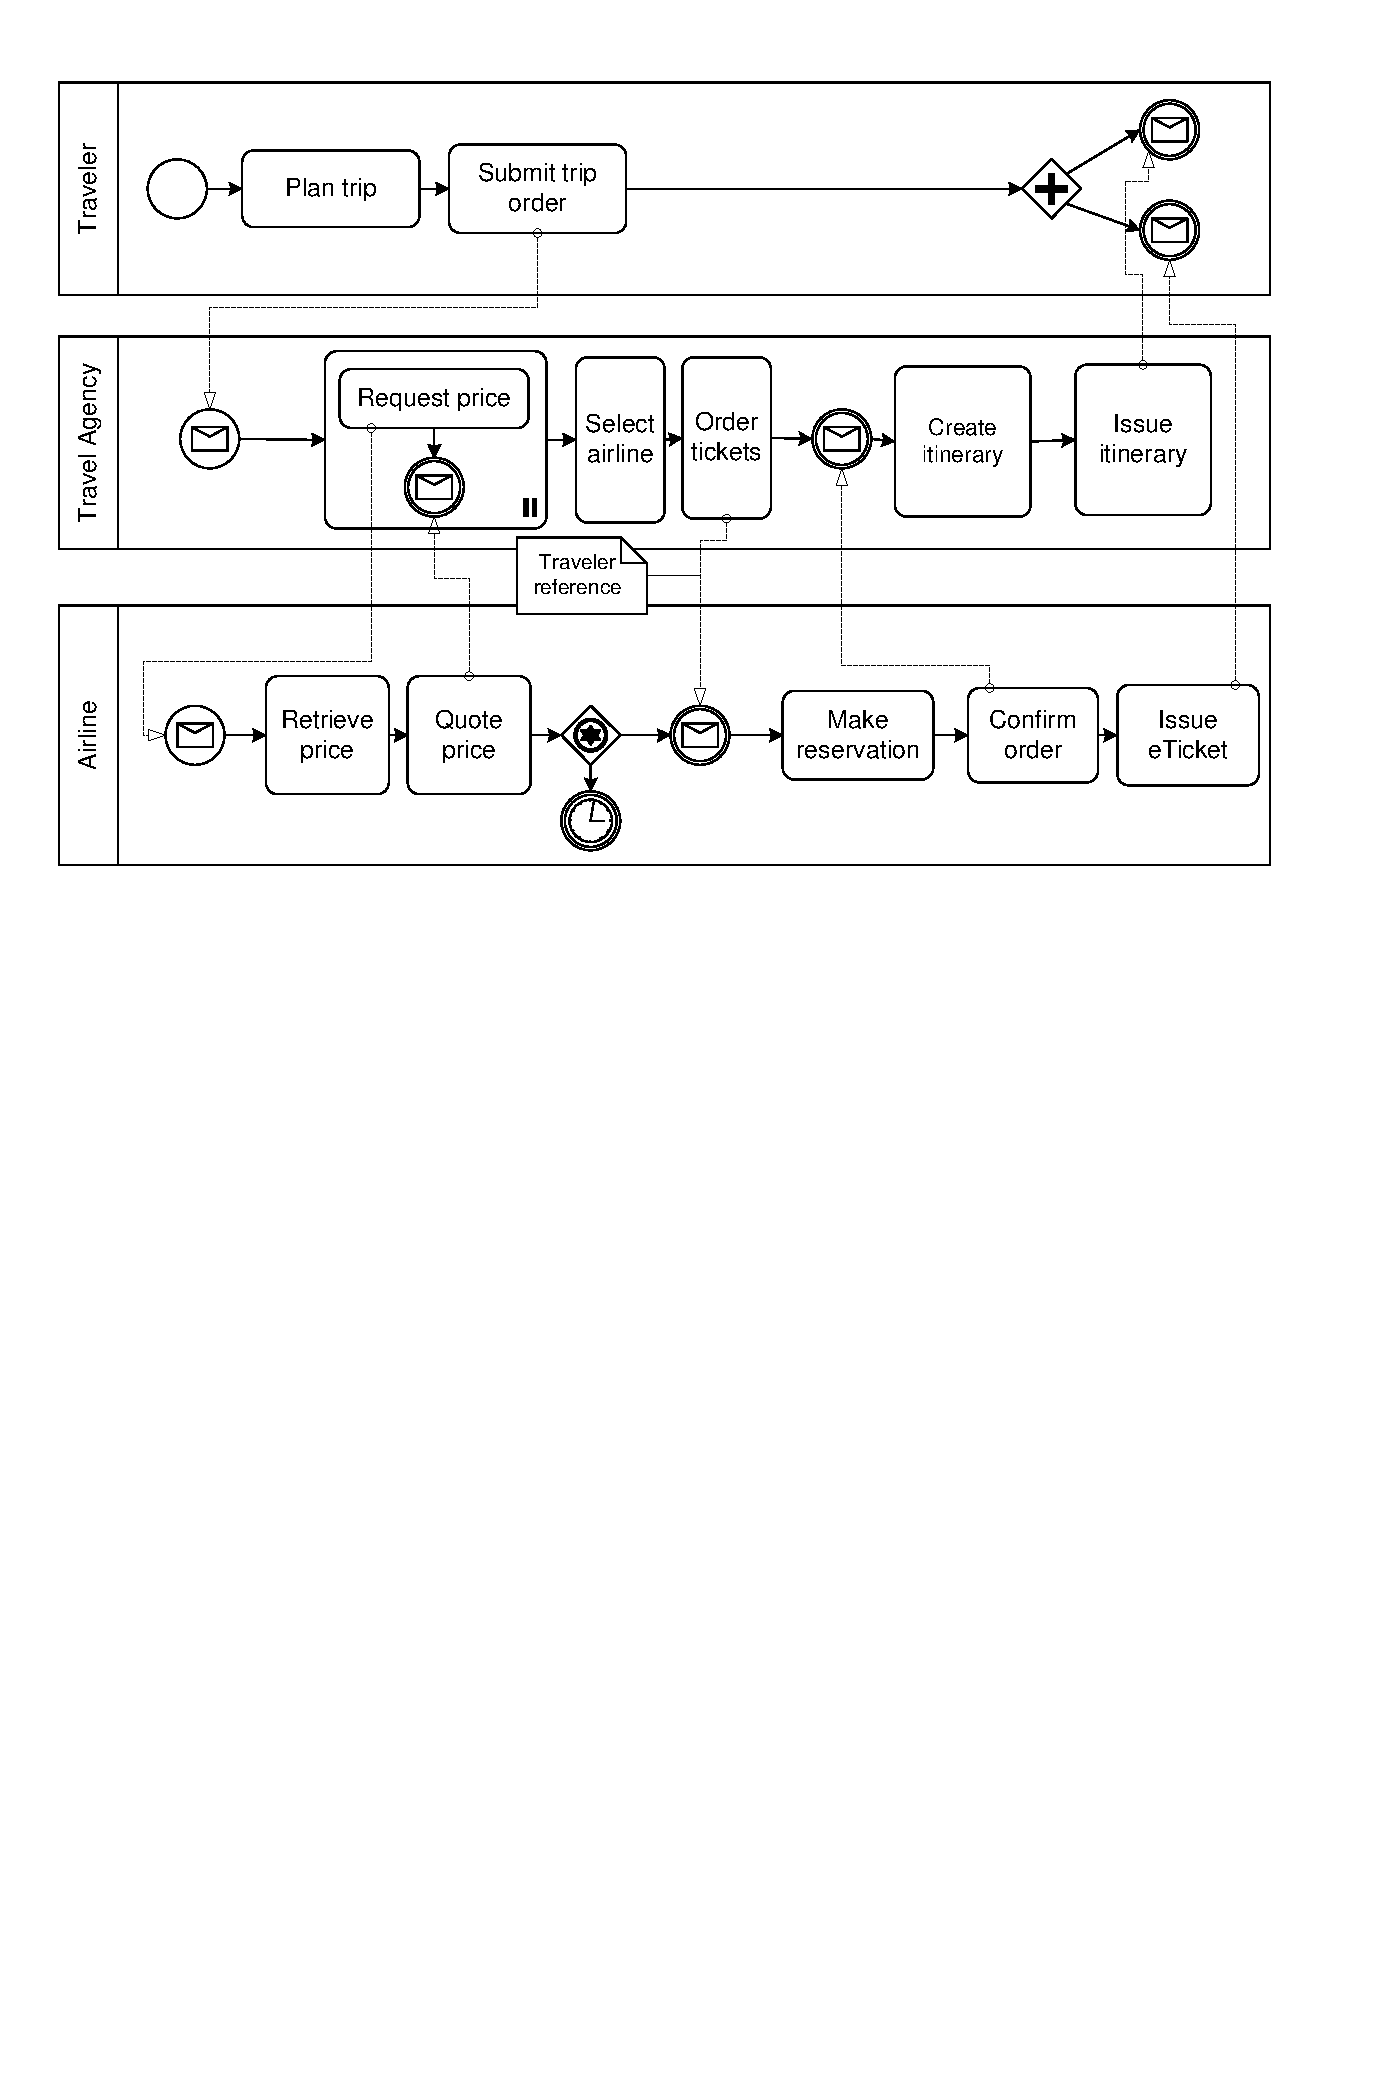
\includegraphics[width=\textwidth]{choreography.pdf}
  \caption{Beispiel-Choreographie}
  \label{fig:chor1}
\end{figure}



\begin{figure}
  \centering
  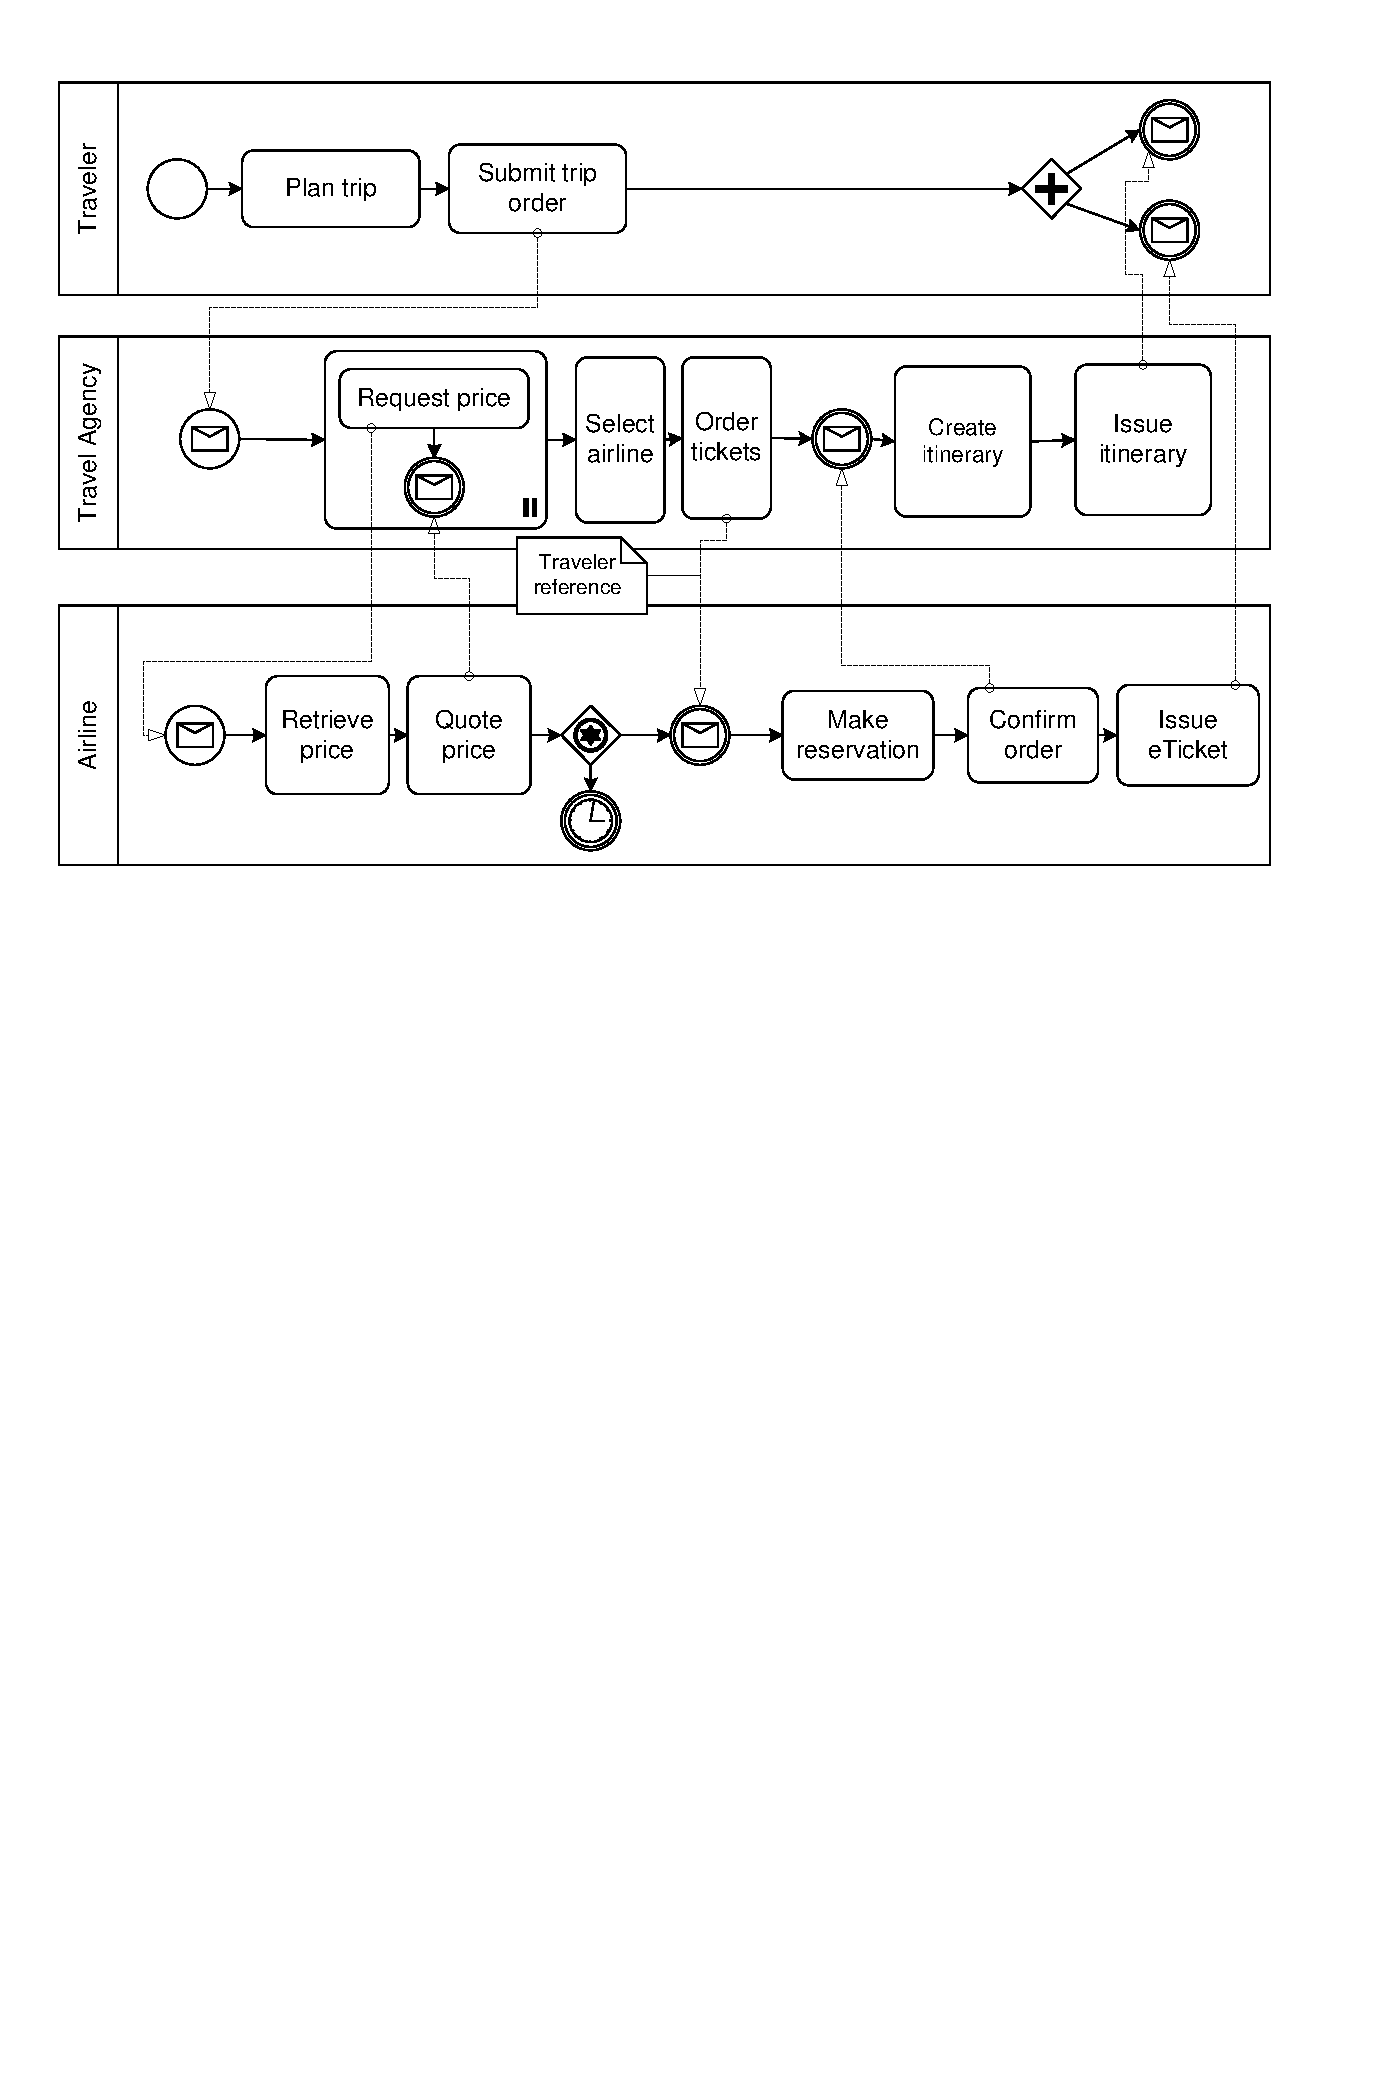
\includegraphics[width=.8\textwidth]{choreography.pdf}
  \caption[Beispiel-Choreographie]{Die Beispiel-Choreographie.
    Nun etwas kleiner, damit \texttt{\textbackslash textwidth} demonstriert wird.
    Und auch die Verwendung von alternativen Bildunterschriften für das Verzeichnis der Abbildungen.
    Letzteres ist allerdings nur Bedingt zu empfehlen, denn wer liest schon so viel Text unter einem Bild?
    Oder ist es einfach nur Stilsache?
  }
  \label{fig:chor2}
\end{figure}


\begin{figure}
  \hfill
  \begin{subfigure}{.3\textwidth}
    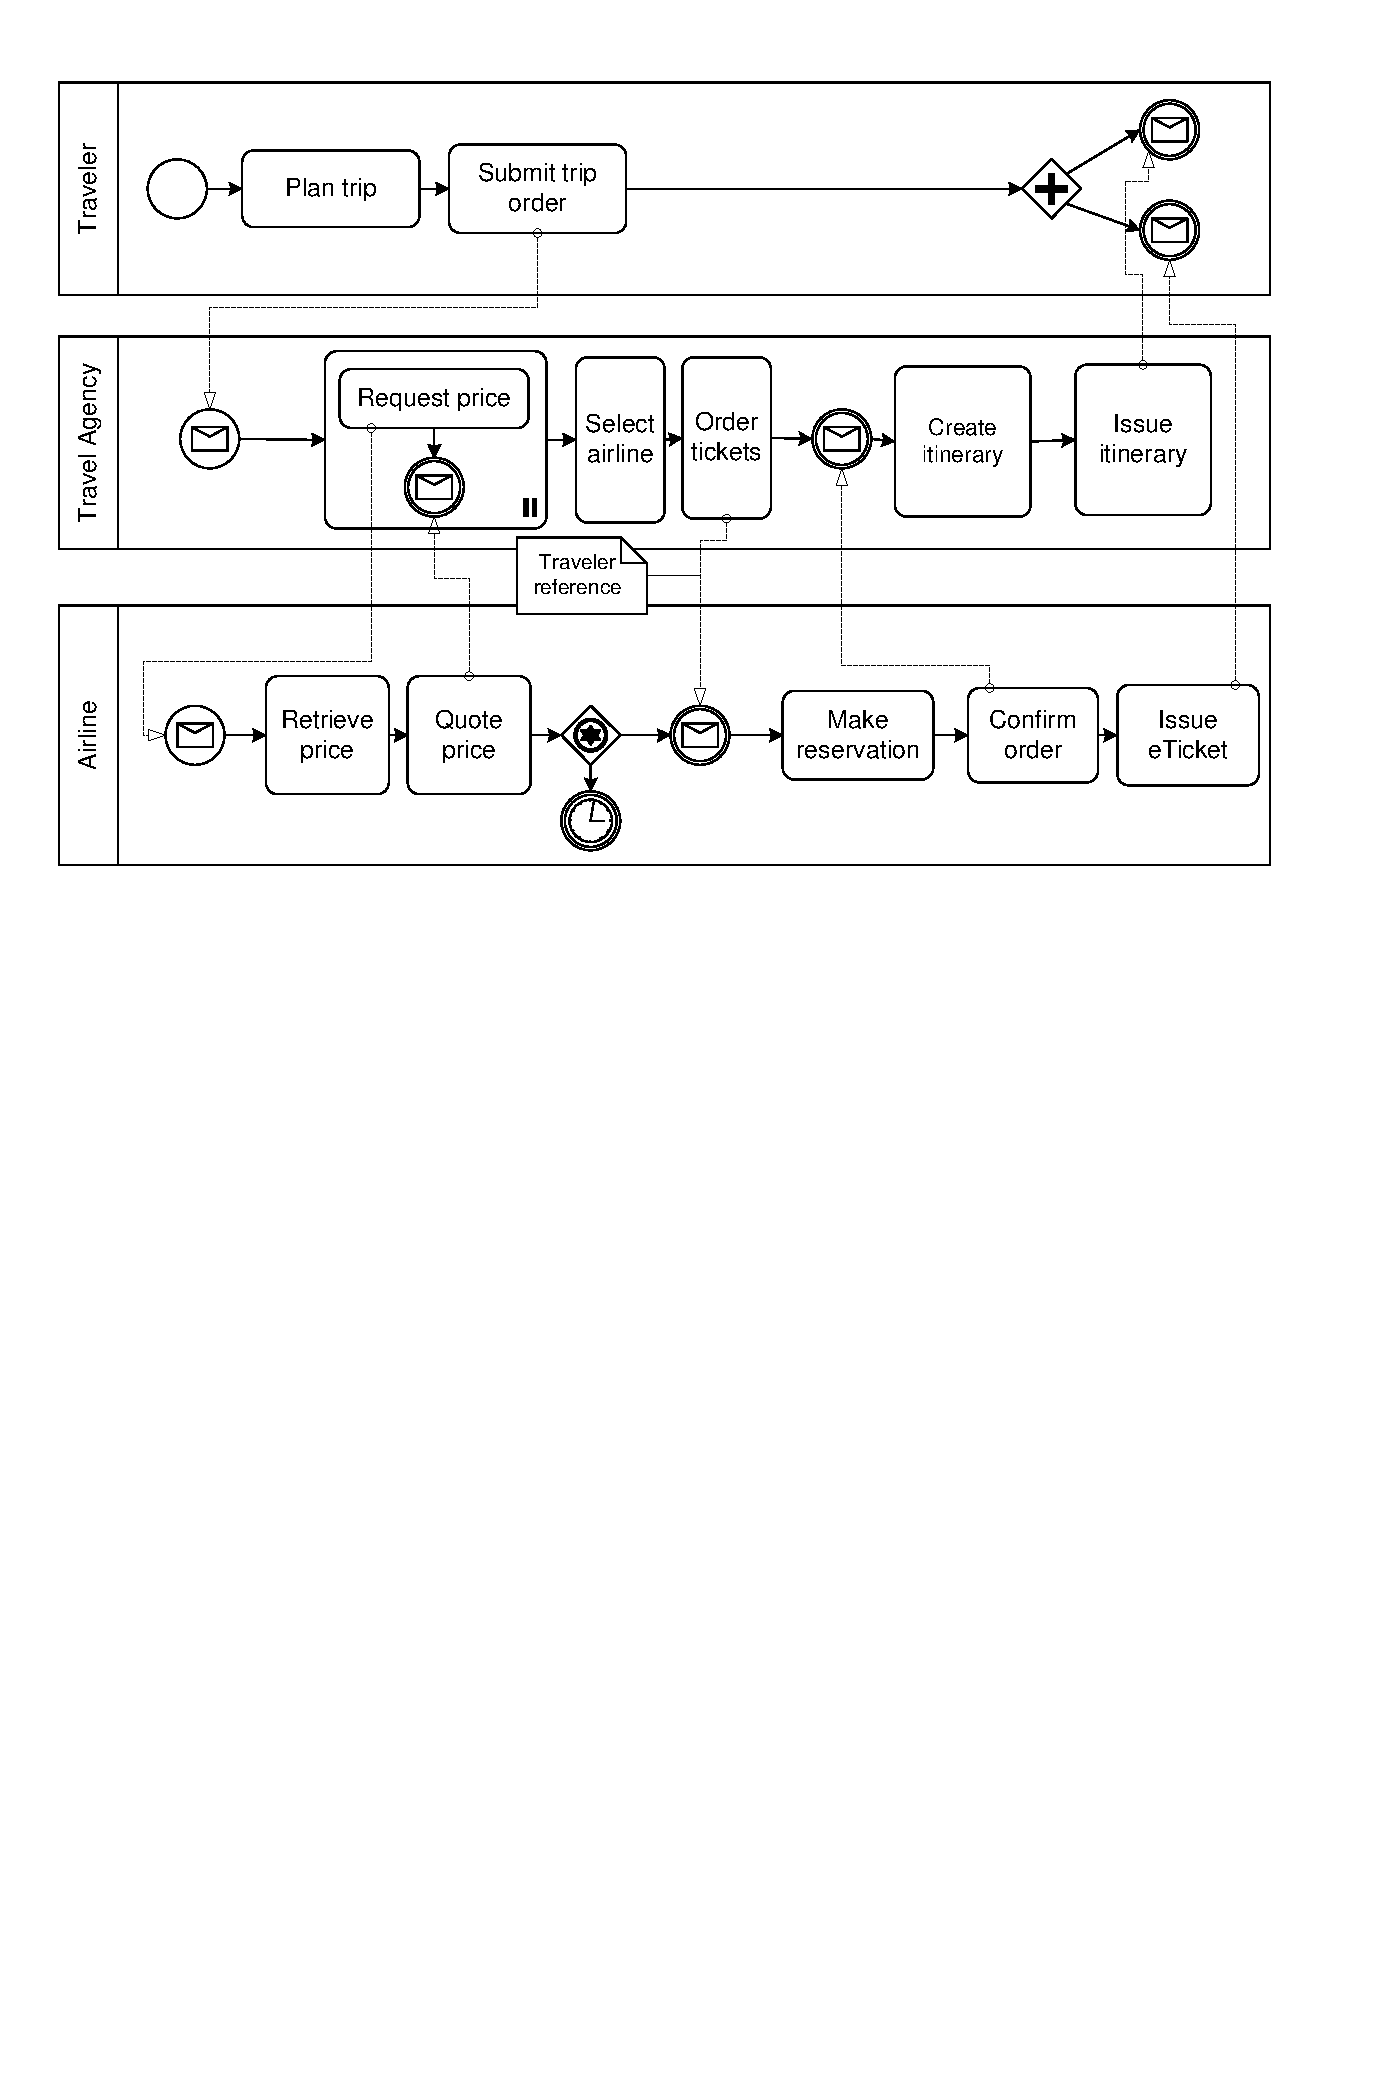
\includegraphics[width=\textwidth]{choreography.pdf}
    \caption{Choreografie 1}
    \label{fig:subfigA}
  \end{subfigure}
  \hfill
  \begin{subfigure}{.3\textwidth}
    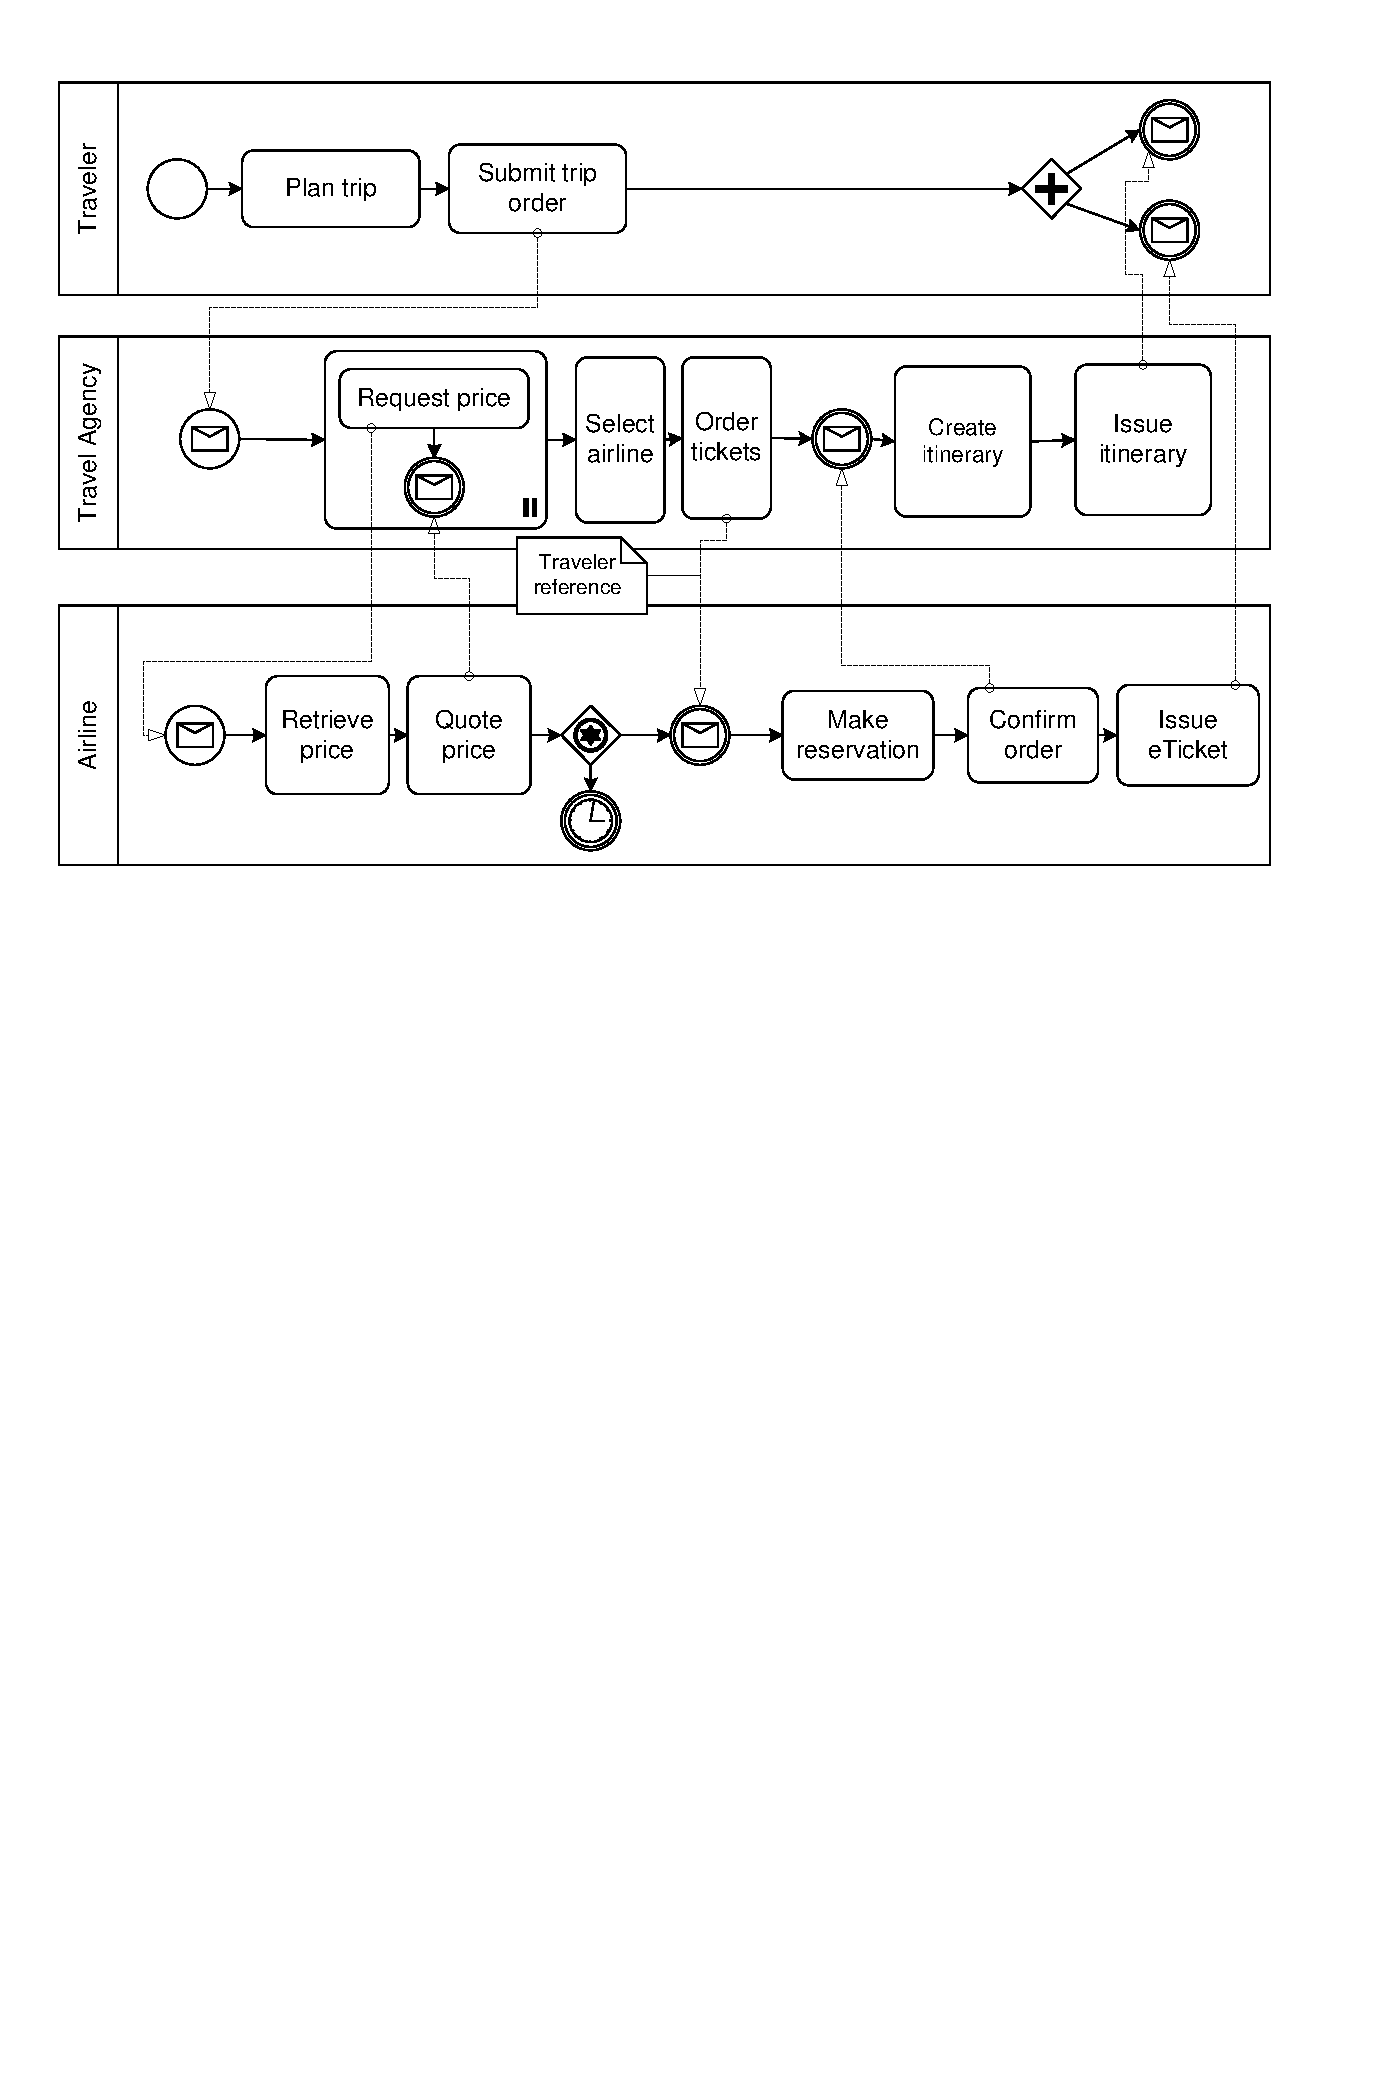
\includegraphics[width=\textwidth]{choreography.pdf}
    \caption{Choreografie 2}
    \label{fig:subfigB}
  \end{subfigure}
  \hfill
  \begin{subfigure}{.3\textwidth}
    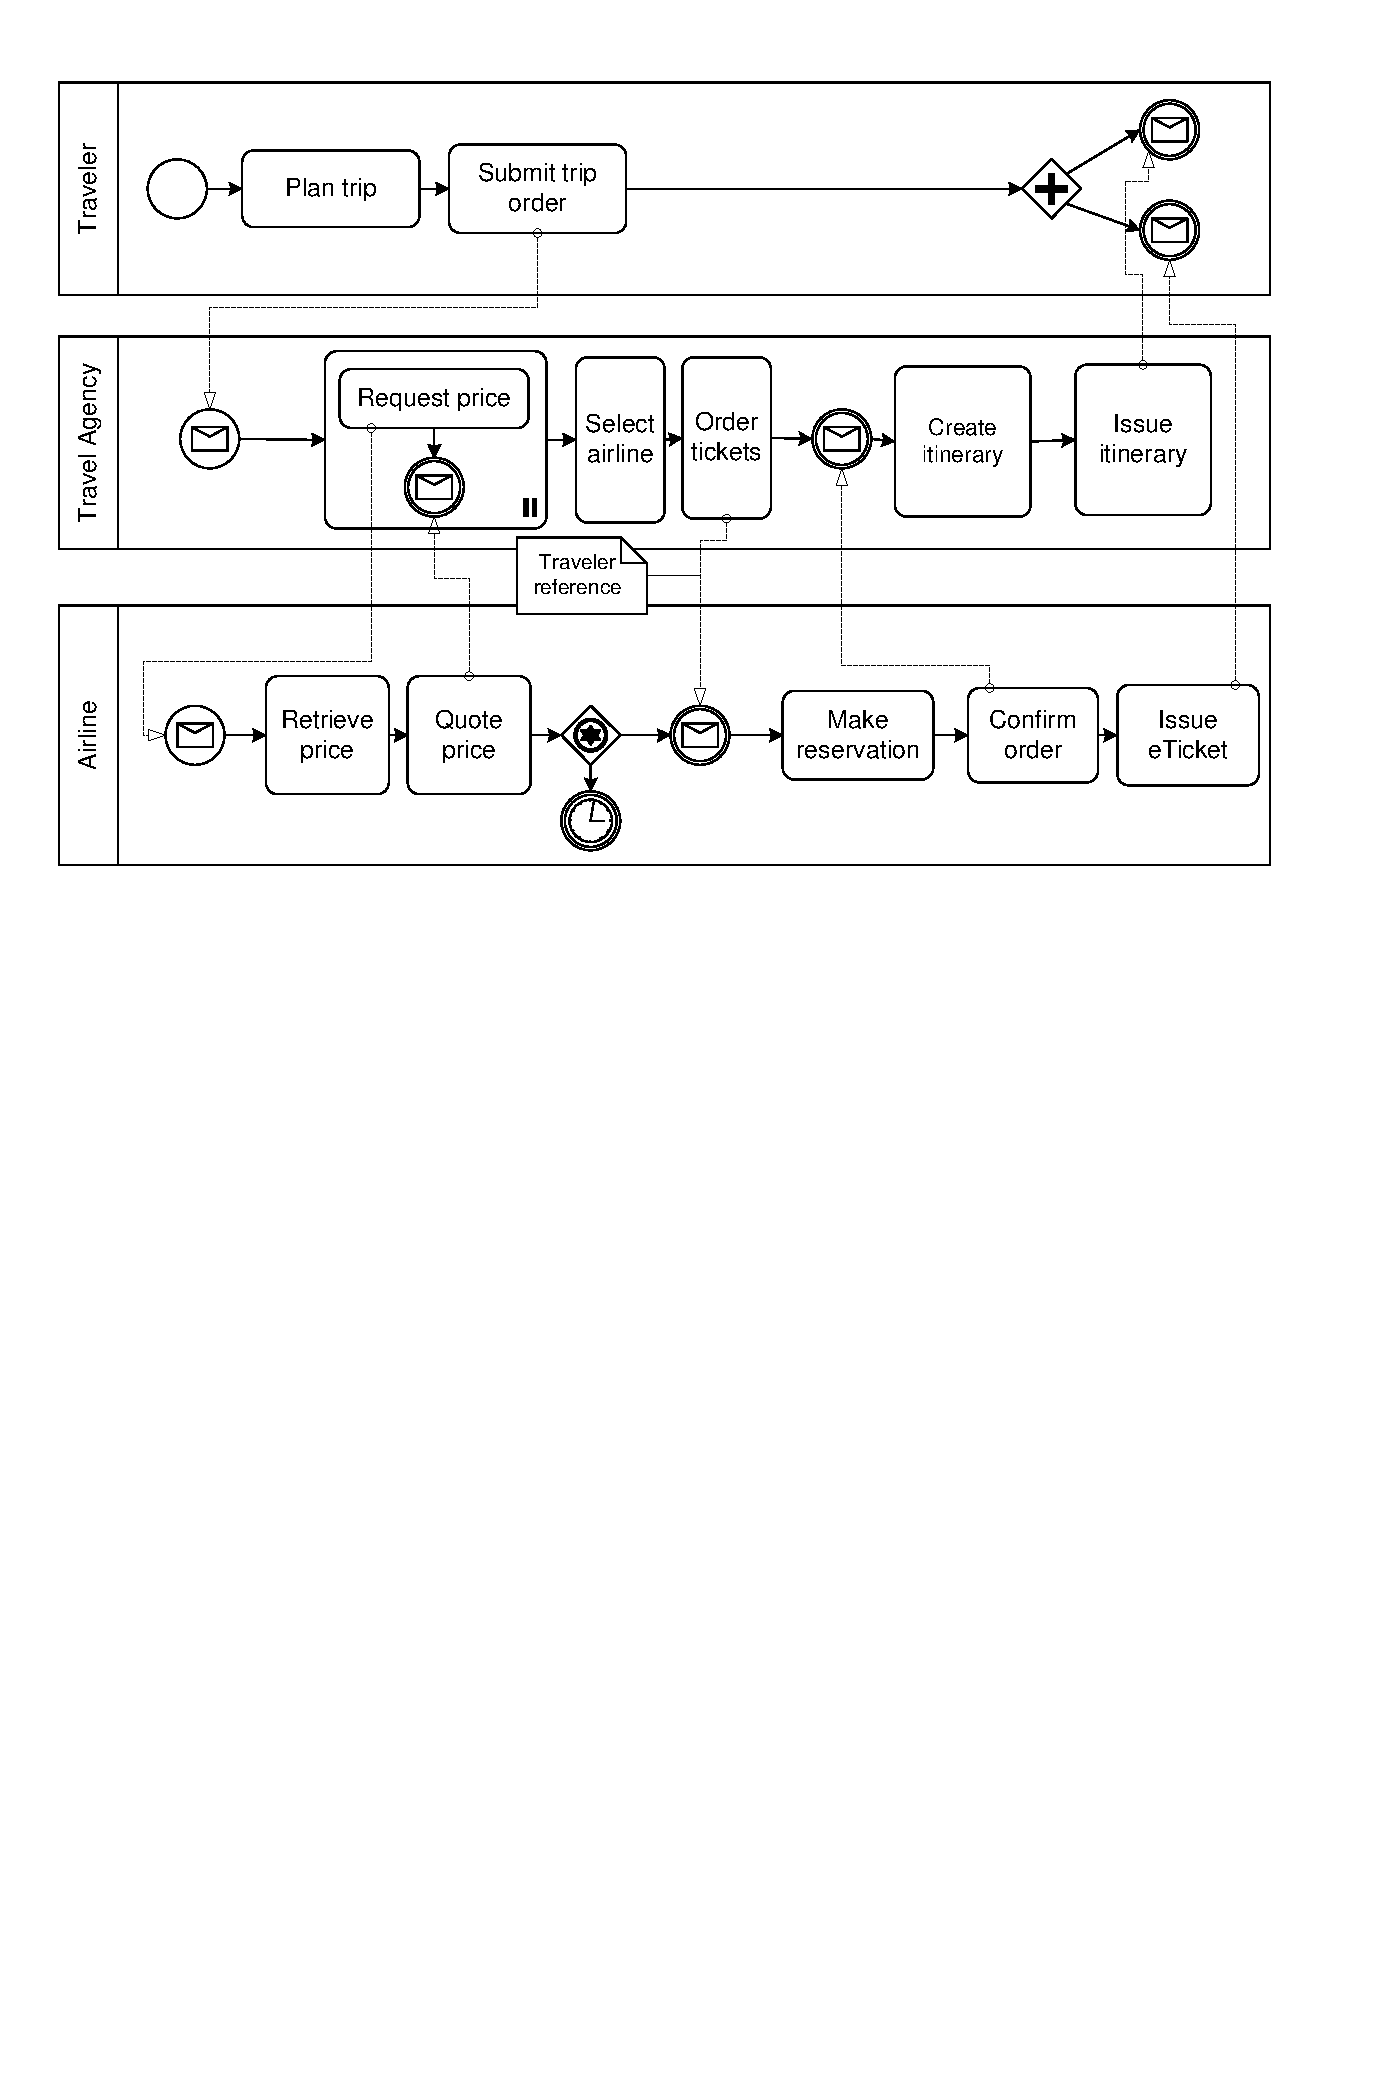
\includegraphics[width=.9\textwidth]{choreography.pdf}
    \caption{Choreografie 3}
    \label{fig:subfigC}
  \end{subfigure}
  \caption{Beispiel um 3 Abbildung nebeneinader zu stellen nur jedes einzeln referenzieren zu können.}
  \label{fig:subfig_example}
\end{figure}

\Cref{fig:subfig_example} zeigt die Verwendung des subcaption-Pakets.
Es ist auch möglich, auf Unterabbildungen zu verweisen: \Cref{fig:subfigA}.

Es ist möglich, SVGs direkt beim Kompilieren in PDF umzuwandeln.
Dies ist im Quellcode zu latex-tipps.tex beschrieben, allerdings auskommentiert.

\iffalse % <-- Das hier wegnehmen, falls inkscape im Pfad ist
  Das SVG in \cref{fig:directSVG} ist direkt eingebunden, während der Text im SVG in \cref{fig:latexSVG} mittels pdflatex gesetzt ist.
  Falls man die Graphiken sehen möchte, muss inkscape im PATH sein und im Tex-Quelltext \texttt{\textbackslash{}iffalse} und \texttt{\textbackslash{}iftrue} auskommentiert sein.

  \begin{figure}
    \centering
    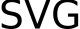
\includegraphics{svgexample.svg}
    \caption{SVG direkt eingebunden}
    \label{fig:directSVG}
  \end{figure}

  \begin{figure}
    \centering
    \def\svgwidth{.4\textwidth}
    \includesvg{svgexample}
    \caption{Text im SVG mittels \LaTeX{} gesetzt}
    \label{fig:latexSVG}
  \end{figure}
\fi % <-- Das hier wegnehmen, falls inkscape im Pfad ist


\section{Weitere Illustrationen}
\Cref{fig:AnhangsChor,fig:AnhangsChor2} zeigen zwei Choreographien, die den Sachverhalt weiter erläutern sollen.
Die zweite Abbildung ist um 90 Grad gedreht, um das Paket \texttt{pdflscape} zu demonstrieren.

\begin{figure}
  \centering
  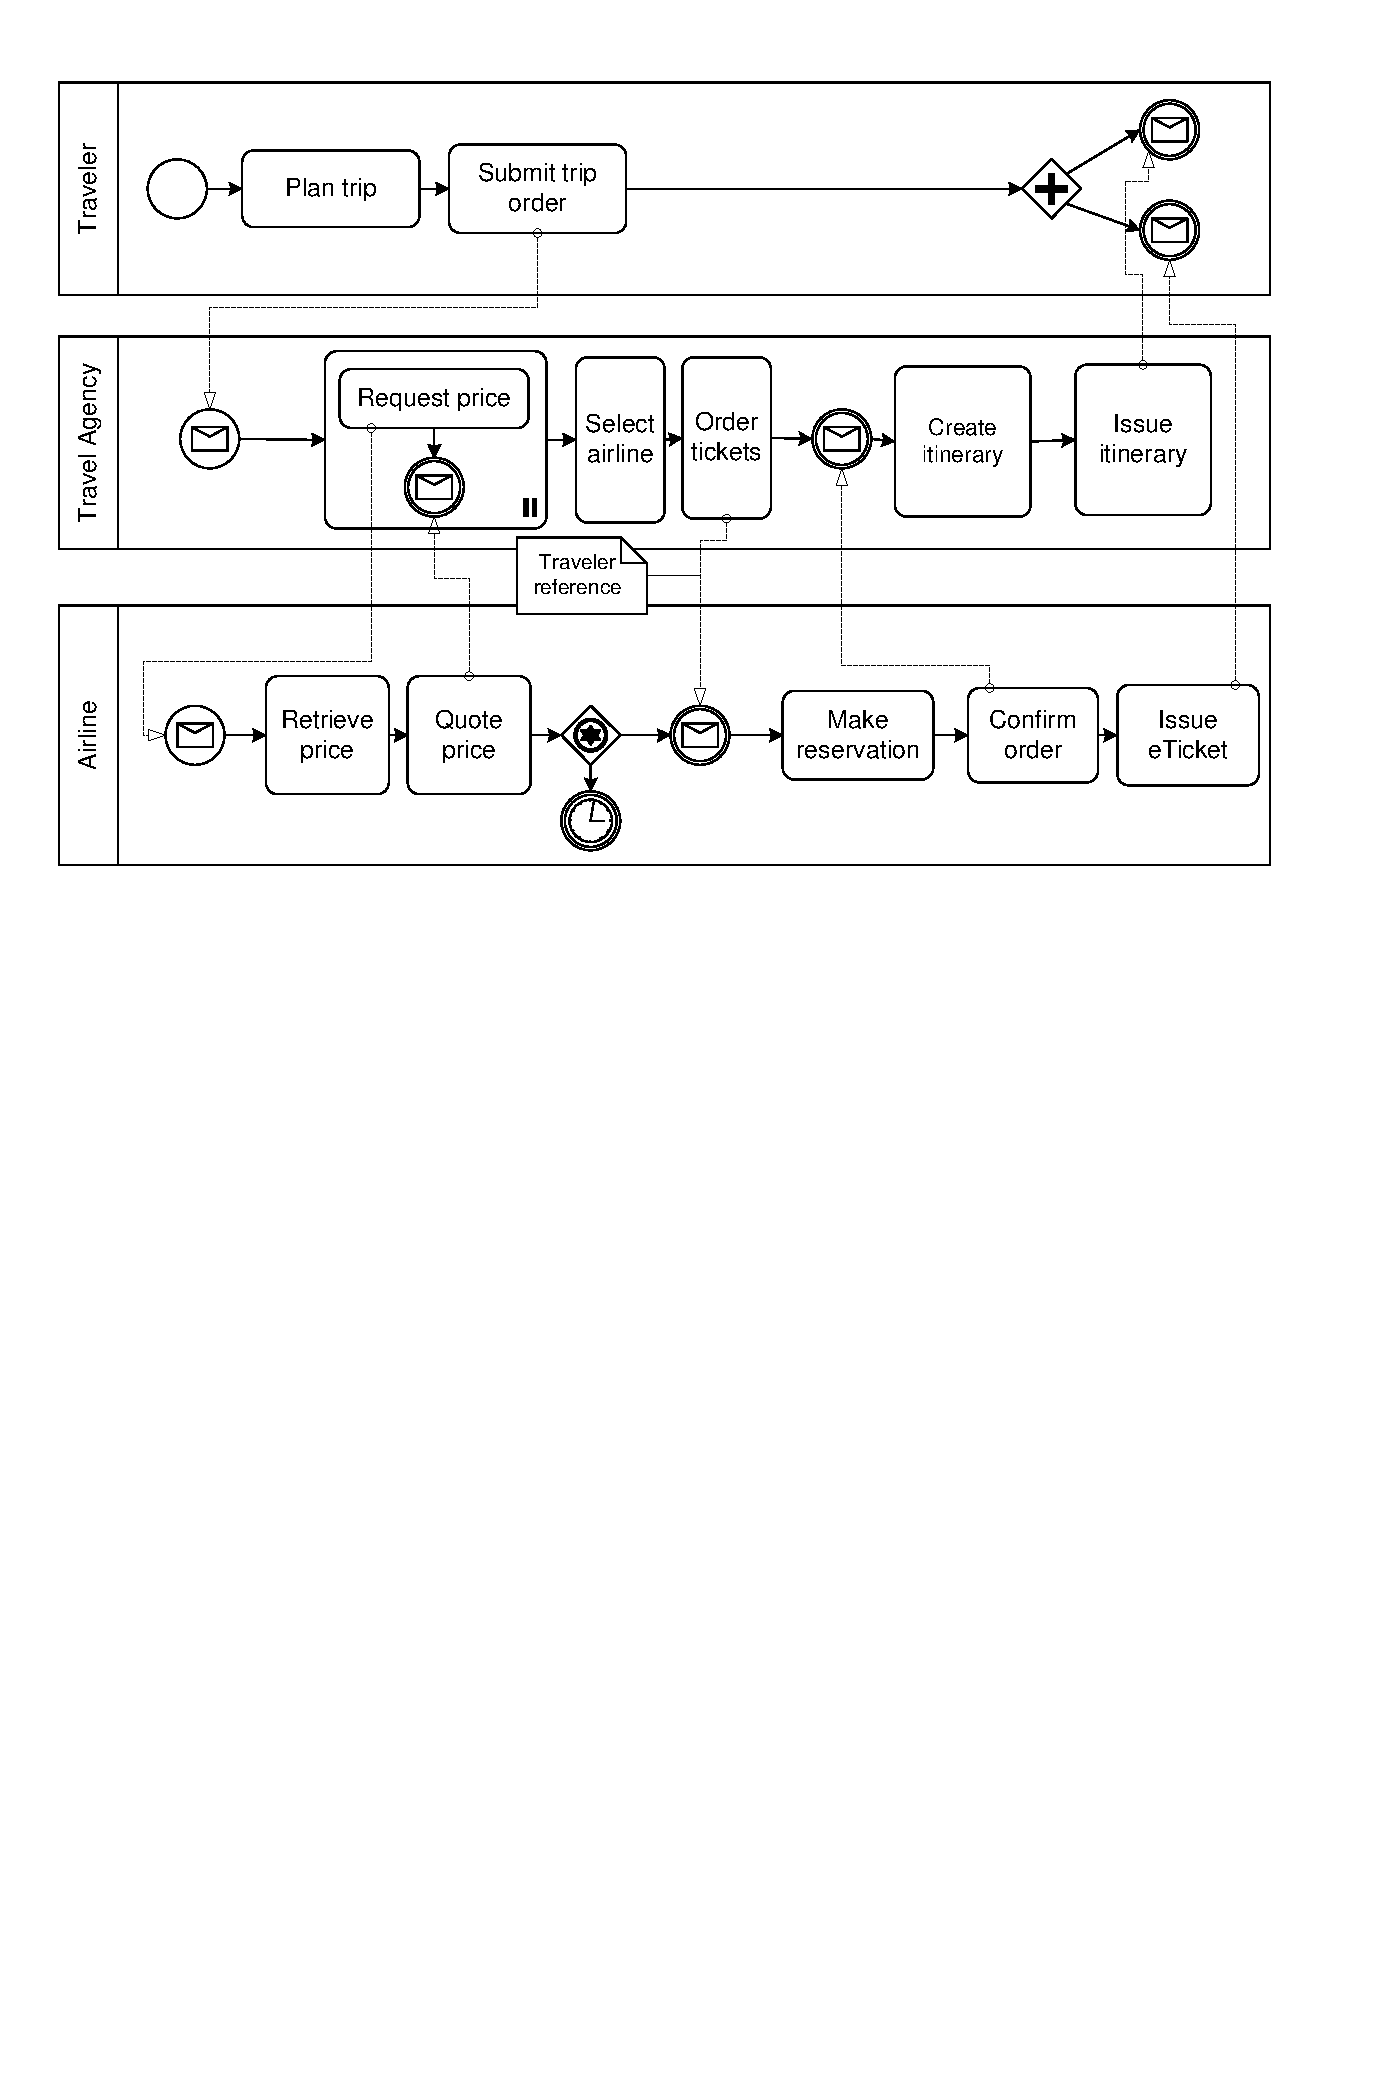
\includegraphics[width=\textwidth]{choreography.pdf}
  \caption{Beispiel-Choreographie I}
  \label{fig:AnhangsChor}
\end{figure}

\begin{landscape}
  \begin{figure}
    \centering
    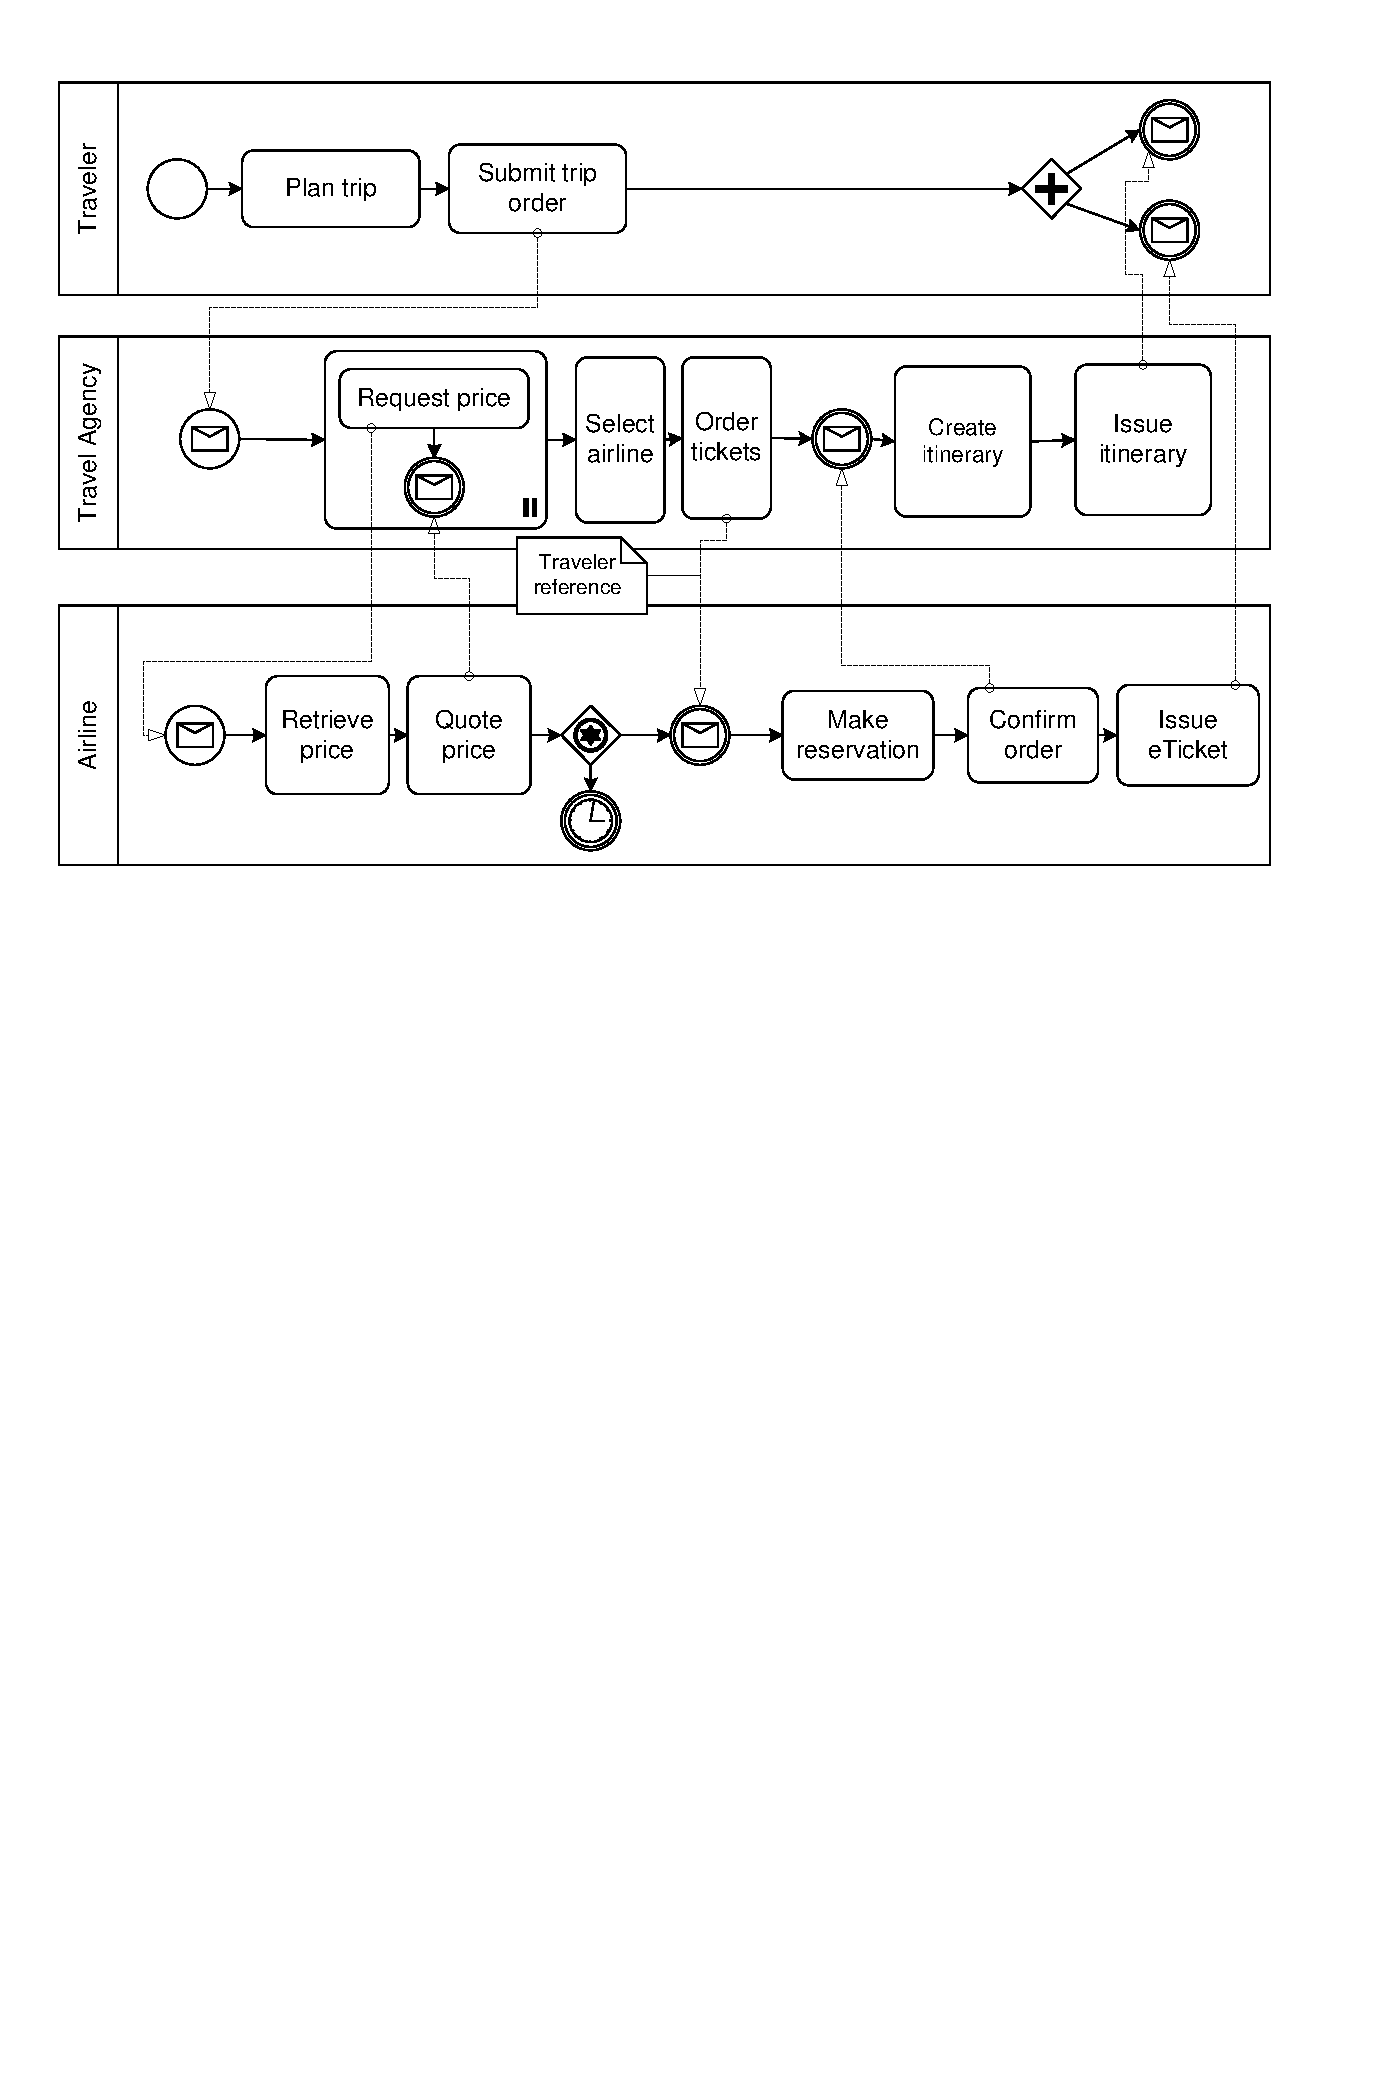
\includegraphics[width=\textwidth]{choreography.pdf}
    \caption{Beispiel-Choreographie II}
    \label{fig:AnhangsChor2}
  \end{figure}
\end{landscape}


\iffalse

  \clearpage

  FIXME - This does not work with MiKTeX as of 2016-12-30

  TODO- demonstrate rotating package

  %hint by http://tex.stackexchange.com/a/3265/9075
  %other option is to use changepage according to http://tex.stackexchange.com/a/2639/9075. This, however, has issues with landscape
  \thispagestyle{empty}

  \savegeometry{koma}

  %If you only have height problems, this is not needed at all
  \addtolength{\textwidth}{2cm}
  \addtolength{\evensidemargin}{-1cm}

  \begin{landscape}
    %sidewaysfigure
    \begin{figure}
      \centering
      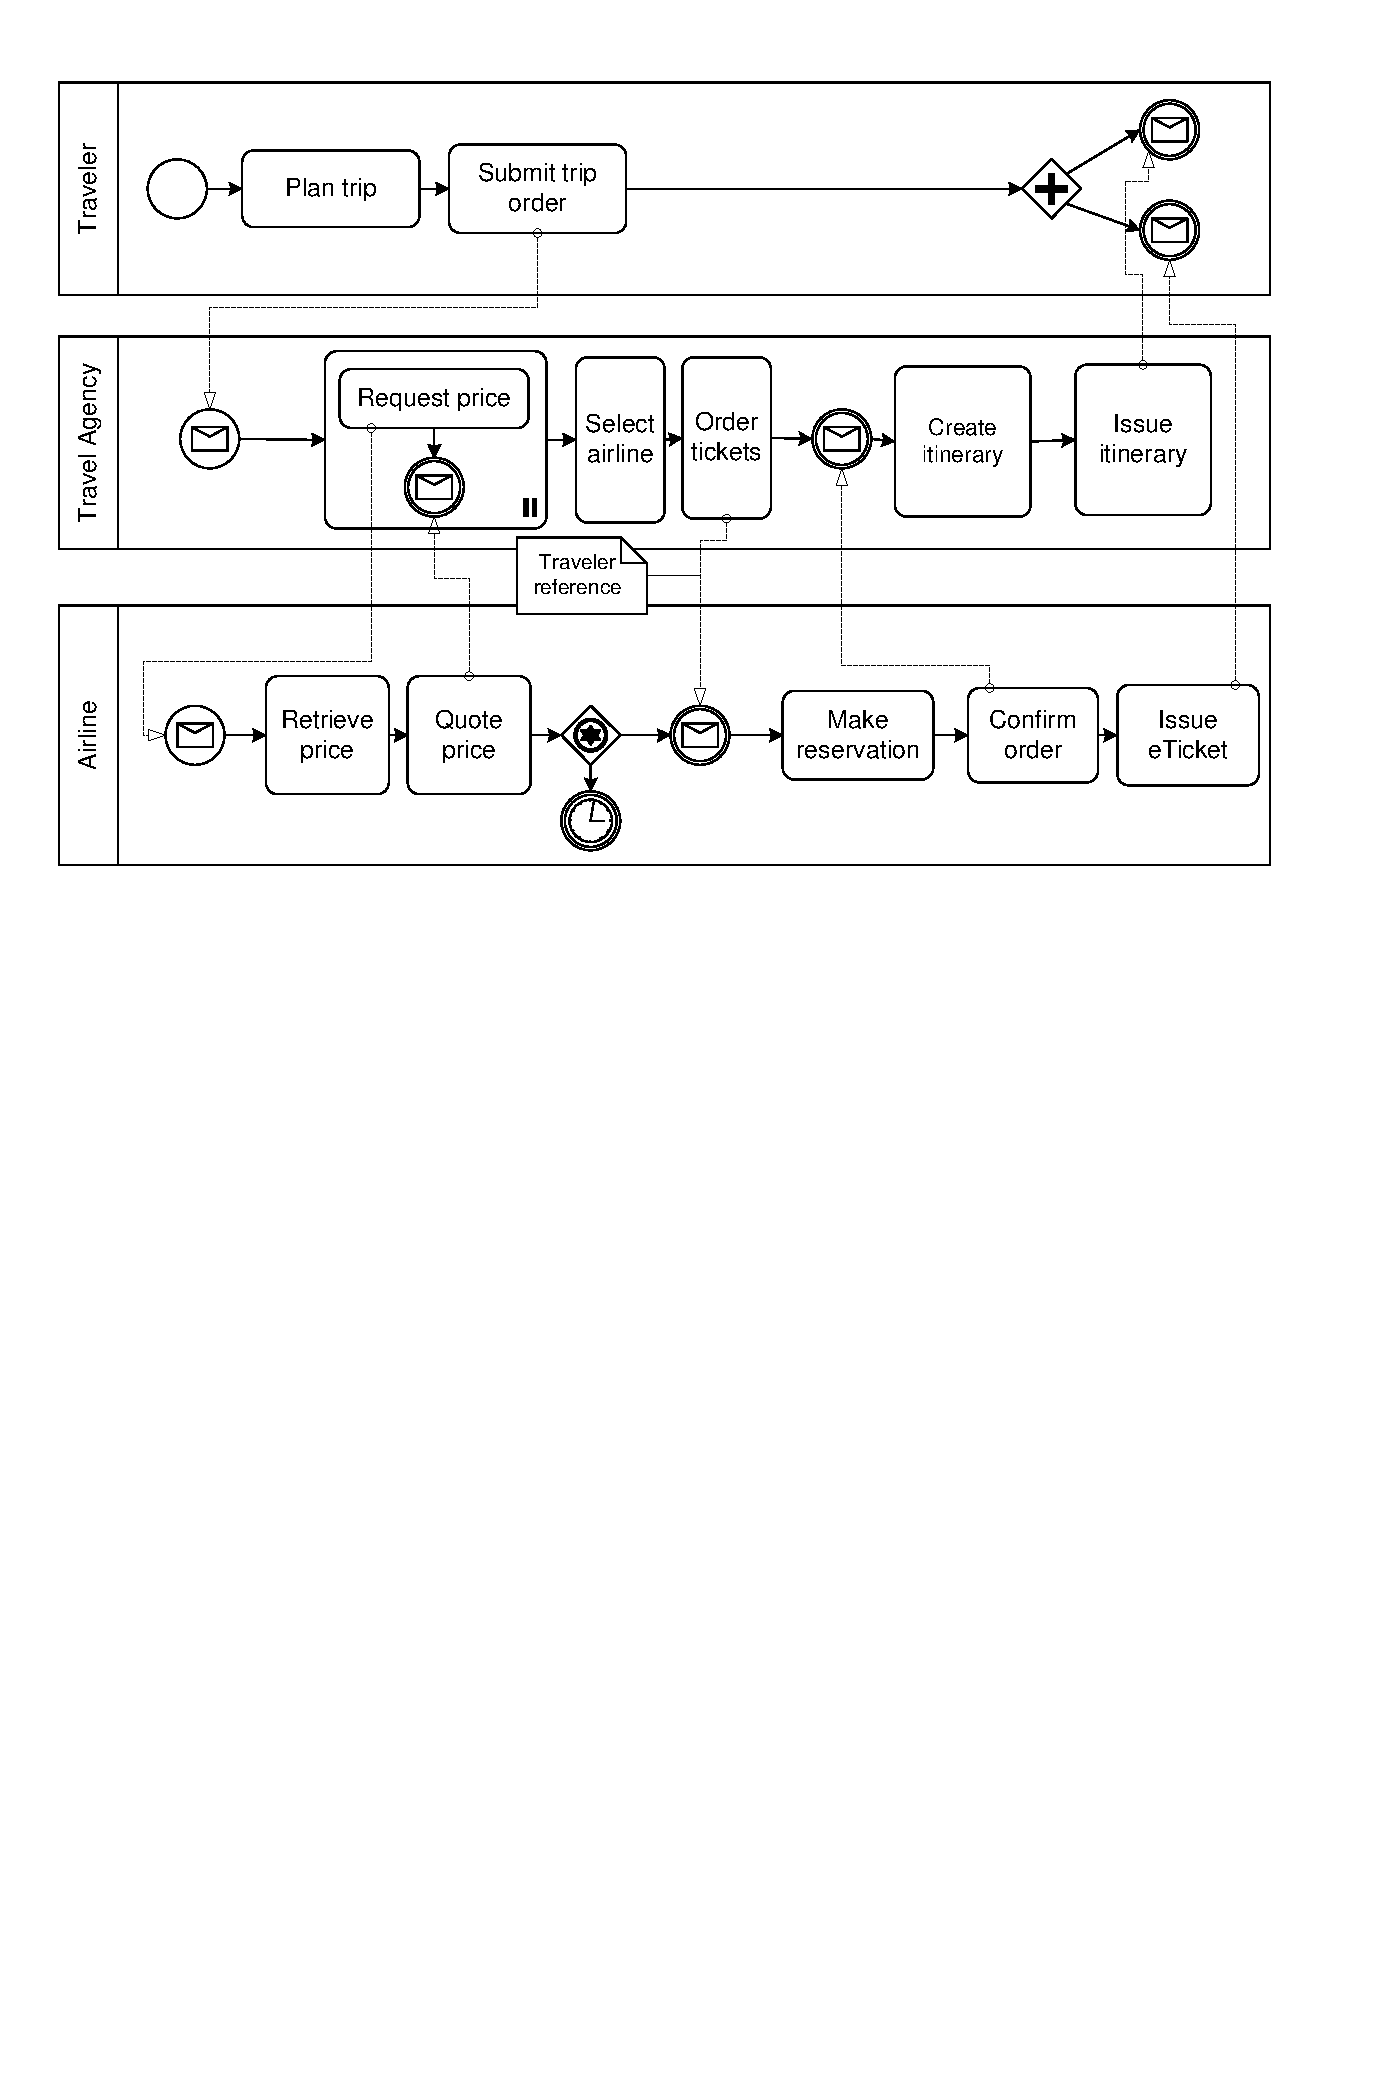
\includegraphics[width=0.9\paperheight]{choreography.pdf}
      \caption{Beispiel-Choreographie, auf einer weißen Seite gezeigt wird und über die definierten Seitenränder herausragt}
    \end{figure}
  \end{landscape}

  %the original layout is restored.
  %%\restoregeometry cannot be used as we use \addtolength
  \loadgeometry{koma}

\fi

\IfFileExists{pgfplots.sty}{
  \section{Plots with pgfplots}
  Pgfplot ist ein Paket um Graphen zu plotten ohne den Umweg über gnuplot oder matplotlib zu gehen.
  %hint by http://tex.stackexchange.com/a/3265/9075%other option is to use changepage according to http://tex.stackexchange.com/a/2639/9075. This, however, has issues with landscape%If you only have height problems, this is not needed at all%sidewaysfigure%the original layout is restored.%%\restoregeometry cannot be used as we use \addtolength
  \begin{figure}[h]
    \begin{center}
      \begin{tikzpicture}
        \begin{axis}[xlabel=$x$,
            ylabel=$\sin(x)$]
          \addplot {sin(deg(x))};  % Sinus-Funktion zeichnen
        \end{axis}
      \end{tikzpicture}
    \end{center}
    \caption{$\sin(x)$ mit pgfplots.}
  \end{figure}

   \begin{figure}[h]
    \begin{center}
      \begin{tikzpicture}
        \begin{axis}[xlabel=$x$,
            ylabel=$y$]
          \addplot table [x=a, y=c, col sep=comma] {data/data.csv};  % Koordinaten aus einer CSV-Datei lesen und plotten
        \end{axis}
      \end{tikzpicture}
    \end{center}
    \caption{Koordianten $x$ und $y$ aus einer CSV-Datei geplottet mit pgfplots.}
  \end{figure}

}{}

\section{Figures with tikz}
TikZ ist ein Paket um Zeichnungen mittels Programmierung zu erstellen.
Dieses Paket eignet sich um Gitter zu erstellen oder andere regelmäßige Strukturen zu erstellen.
Hier gibt es sehr viele visuelle Beispiele was tikz alles kann\footnote{\url{http://texdoc.net/pkg/visualtikz}}.

\begin{figure}[ht]
  \begin{center}
    \begin{tikzpicture}
      \draw(0,0) rectangle (4,4);
      \foreach \x in {0.5,1,1.5,2,2.5,3,3.5}
      \foreach \y in {0.5,1,1.5,2,2.5,3,3.5}
      \draw(\x,\y) circle (1pt);
    \end{tikzpicture}
  \end{center}
  \caption{Eine tikz-Graphik.}\label{fig:tikz_example}
\end{figure}


\section{UML-Diagramme mit tikz-uml}

\Cref{fig:uml} zeigt ein Klassendiagramm, das mittels tikz-uml gesetzt wurde.

\begin{center}
\begin{figure}
\begin{tikzpicture}
\begin{umlpackage}{p}
\begin{umlpackage}{sp1}
\umlclass[template=T]{A}{
  n : uint \\ t : float
}{}
\umlclass[y=-3]{B}{
  d : double
}{
  \umlvirt{setB(b : B) : void} \\ getB() : B}
\end{umlpackage}
\begin{umlpackage}[x=10,y=-6]{sp2}
\umlinterface{C}{
  n : uint \\ s : string
}{}
\end{umlpackage}
\umlclass[x=2,y=-10]{D}{
  n : uint
  }{}
\end{umlpackage}

\umlassoc[geometry=-|-, arg1=tata, mult1=*, pos1=0.3, arg2=toto, mult2=1, pos2=2.9, align2=left]{C}{B}
\umlunicompo[geometry=-|, arg=titi, mult=*, pos=1.7, stereo=vector]{D}{C}
\umlimport[geometry=|-, anchors=90 and 50, name=import]{sp2}{sp1}
\umlaggreg[arg=tutu, mult=1, pos=0.8, angle1=30, angle2=60, loopsize=2cm]{D}{D}
\umlinherit[geometry=-|]{D}{B}
\umlnote[x=2.5,y=-6, width=3cm]{B}{Eine Notiz f\"ur die Klasse B}
\umlnote[x=7.5,y=-2]{import-2}{Eine Anmerkung}
\end{tikzpicture}
\caption{Ein Klassendiagramm mit tikz-uml generiert. Beispiel von Nicolas Kielbasiewicz adaptiert.}
\label{fig:uml}
\end{figure}
\end{center}

\section{Tabellen}

\cref{tab:Ergebnisse} zeigt Ergebnisse und die \cref{tab:Ergebnisse} zeigt wie numerische Daten in einer Tabelle representiert werden können.
\begin{table}
  \centering
  \begin{tabular}{ccc}
    \toprule
    \multicolumn{2}{c}{\textbf{zusammengefasst}} & \textbf{Titel}                                                          \\ \midrule
    Tabelle                                      & wie                                                           & in      \\
    \url{tabsatz.pdf}                            & empfohlen                                                     & gesetzt \\

    \multirow{2}{*}{Beispiel}                    & \multicolumn{2}{c}{ein schönes Beispiel}                                \\
                                                 & \multicolumn{2}{c}{für die Verwendung von \qq{multirow}}           \\
    \bottomrule
  \end{tabular}
  \caption[Beispieltabelle]{Beispieltabelle -- siehe \url{http://www.ctan.org/tex-archive/info/german/tabsatz/}}
  \label{tab:Ergebnisse}
\end{table}

\begin{table}
  \centering
  \begin{tabular}{l *{8}{d{3.2}}}
    \toprule

                         & \multicolumn{2}{c}{\textbf{Parameter 1}} & \multicolumn{2}{c}{\textbf{Parameter 2}} & \multicolumn{2}{c}{\textbf{Parameter 3}} & \multicolumn{2}{c}{\textbf{Parameter 4}}                                                                                                                                       \\
    \cmidrule(r){2-3}\cmidrule(lr){4-5}\cmidrule(lr){6-7}\cmidrule(l){8-9}

    \textbf{Bedingungen} & \multicolumn{1}{c}{\textbf{M}}           & \multicolumn{1}{c}{\textbf{SD}}          & \multicolumn{1}{c}{\textbf{M}}           & \multicolumn{1}{c}{\textbf{SD}}          & \multicolumn{1}{c}{\textbf{M}} & \multicolumn{1}{c}{\textbf{SD}} & \multicolumn{1}{c}{\textbf{M}} & \multicolumn{1}{c}{\textbf{SD}} \\
    \midrule

    W                    & 1.1                                      & 5.55                                     & 6.66                                     & .01                                      &                                &                                 &                                &                                 \\
    X                    & 22.22                                    & 0.0                                      & 77.5                                     & .1                                       &                                &                                 &                                &                                 \\
    Y                    & 333.3                                    & .1                                       & 11.11                                    & .05                                      &                                &                                 &                                &                                 \\
    Z                    & 4444.44                                  & 77.77                                    & 14.06                                    & .3                                       &                                &                                 &                                &                                 \\
    \bottomrule
  \end{tabular}

  \caption{
    Beispieltabelle f\"{u}r 4 Bedingungen (W-Z) mit jeweils 4 Parameters mit (M und SD).
    Hinweis: Stets die selbe Anzahl an Nachkommastellen angeben.
  }
  \label{tab:Werte}
\end{table}



\IfFileExists{pgfplotstable.sty}{

\subsection{Tabellen mit pgfplots}
Mit pgfplots koennen Tabellen direkt aus einer CSV-Datei erstellt werden.

\begin{table}[h]
\centering
\pgfplotstabletypeset[
col sep = comma,
every head row/.style={before row=\toprule,after row=\midrule},
every last row/.style={after row=\bottomrule},
display columns/0/.style={string type,column name={}}
]
{data/data.csv}
\caption{Tabelle generiert aus einer CSV-Datei mit pgfplots}
\end{table}
}{}


\section{Tabellen über mehere Seiten}

\begin{longtable}{|l|l|l|}
\caption{Tabelle \"uber mehere Seiten} \label{tab:long} \\

\hline \multicolumn{1}{|c|}{\textbf{A}} & \multicolumn{1}{c|}{\textbf{B}} & \multicolumn{1}{c|}{\textbf{B}} \\ \hline
\endfirsthead

\multicolumn{3}{c}%
{{\bfseries \tablename\ \thetable{} -- von dor vorherigen Seite weitergeführt}} \\
\hline \multicolumn{1}{|c|}{\textbf{First column}} & \multicolumn{1}{c|}{\textbf{Second column}} & \multicolumn{1}{c|}{\textbf{Third column}} \\ \hline
\endhead

\hline \multicolumn{3}{|r|}{{Wird auf der n\"achsten Seite fortgef\"uhrt}} \\ \hline
\endfoot

\hline \hline
\endlastfoot

A & B C & D \\
A & B C & D \\
A & B C & D \\
A & B C & D \\
A & B C & D \\
A & B C & D \\
A & B C & D \\
A & B C & D \\
A & B C & D \\
A & B C & D \\
A & B C & D \\
A & B C & D \\
A & B C & D \\
A & B C & D \\
A & B C & D \\
A & B C & D \\
A & B C & D \\
A & B C & D \\
A & B C & D \\
A & B C & D \\
A & B C & D \\
A & B C & D \\
A & B C & D \\
A & B C & D \\
A & B C & D \\
A & B C & D \\
A & B C & D \\
A & B C & D \\
A & B C & D \\
A & B C & D \\
A & B C & D \\
A & B C & D \\
A & B C & D \\
A & B C & D \\
A & B C & D \\
A & B C & D \\
A & B C & D \\
A & B C & D \\
A & B C & D \\
A & B C & D \\
A & B C & D \\
A & B C & D \\
A & B C & D \\
A & B C & D \\
A & B C & D \\
A & B C & D \\
A & B C & D \\
A & B C & D \\
A & B C & D \\
A & B C & D \\
A & B C & D \\
A & B C & D \\
A & B C & D \\
A & B C & D \\
A & B C & D \\
A & B C & D \\
A & B C & D \\
A & B C & D \\
A & B C & D \\
A & B C & D \\
A & B C & D \\
A & B C & D \\
A & B C & D \\
A & B C & D \\
A & B C & D \\
A & B C & D \\
A & B C & D \\
A & B C & D \\
A & B C & D \\
A & B C & D \\
A & B C & D \\
A & B C & D \\
A & B C & D \\
A & B C & D \\
A & B C & D \\
A & B C & D \\
A & B C & D \\
A & B C & D \\
A & B C & D \\
A & B C & D \\
\end{longtable}


\section{Abkürzungen}

Beim ersten Durchlauf betrug die \gls{fr} 5.
Beim zweiten Durchlauf war die \gls{fr} 3.
Die Pluralform sieht man hier: \glspl{er}.
Um zu demonstrieren, wie das Abkürzungsverzeichnis bei längeren Beschreibungstexten aussieht, muss hier noch \glspl{rdbms} erwähnt werden.

Mit \verb+\gls{...}+ können Abkürzungen eingebaut werden, beim ersten Aufrufen wird die lange Form eingesetzt.
Beim wiederholten Verwenden von \verb+\gls{...}+ wird automatisch die kurz Form angezeigt.
Außerdem wird die Abkürzung automatisch in die Abkürzungsliste eingefügt.
Mit \verb+\glspl{...}+ wird die Pluralform verwendet.
Möchte man, dass bei der ersten Verwendung direkt die Kurzform erscheint, so kann man mit \verb+\glsunset{...}+ eine Abkürzung als bereits verwendet markieren.
Das Gegenteil erreicht man mit \verb+\glsreset{...}+.

Definiert werden Abkürzungen in der Datei \textit{content\\ausarbeitung.tex} mithilfe von \verb+\newacronym{...}{...}{...}+.

Mehr Infos unter: \url{http://tug.ctan.org/macros/latex/contrib/glossaries/glossariesbegin.pdf}


\section{Verweise}
Für weit entfernte Abschnitte ist \qq{varioref} zu empfehlen:
\qq{Siehe \vref{sec:mf}}.
Das Kommando \texttt{\textbackslash{}vref} funktioniert ähnlich wie \texttt{\textbackslash{}cref} mit dem Unterschied, dass zusätzlich ein Verweis auf die Seite hinzugefügt wird.
\texttt{vref}: \qq{\vref{sec:firstsectioninlatexhints}}, \texttt{cref}: \qq{\cref{sec:firstsectioninlatexhints}}, \texttt{ref}: \qq{\ref{sec:firstsectioninlatexhints}}.

Falls \qq{varioref} Schwierigkeiten macht, dann kann man stattdessen \qq{cref} verwenden.
Dies erzeugt auch das Wort \qq{Abschnitt} automatisch: \cref{sec:mf}.
Das geht auch für Abbildungen usw.
Im Englischen bitte \verb1\Cref{...}1 (mit großem \qq{C} am Anfang) verwenden.


%Mit MiKTeX Installation ab dem 2012-01-16 nicht mehr nötig
%Falls ein Abschnitt länger als eine Seite wird und man mittels \texttt{\textbackslash{}vref} auf eine konkrete Stelle in der Section
%verweisen möchte, dann sollte man \texttt{\textbackslash{}phantomsection} verwenden und dann wird
%auch bei \texttt{vref} die richtige Seite angeben.

%%The link location will be placed on the line below.
%%Tipp von http://en.wikibooks.org/wiki/LaTeX/Labels_and_Cross-referencing#The_hyperref_package_and_.5Cphantomsection
%\phantomsection
%\label{alabel}
%Das Beispiel für \texttt{\textbackslash{}phantomsection} bitte im \LaTeX{}-Quellcode anschauen.

%Hier das Beispiel: Siehe Abschnitt \vref{hack1} und Abschnitt \vref{hack2}.


\section{Definitionen}
\begin{definition}[Title]
  \label{def:def1}
  Definition Text
\end{definition}

\Cref{def:def1} zeigt \ldots

\section{Fußnoten}
Fußnoten können mit dem Befehl \verb+\footnote{...}+ gesetzt werden\footnote{\label{fussnote}Diese Fußnote ist ein Beispiel.
}.
Mehrfache Verwendung von Fußnoten ist möglich indem man zu erst ein Label in der Fußnote setzt \verb+\footnote{\label{...}...}+ und anschließend mittels \verb+\cref{...}+ die Fußnote erneut verwendet\cref{fussnote}.


\section{Verschiedenes}
\label{sec:diff}
\ifdeutsch
  Ziffern (123\,654\,789) werden schön gesetzt.
  Entweder in einer Linie oder als Minuskel-Ziffern.
  Letzteres erreicht man durch den Parameter \texttt{osf} bei dem Paket \texttt{libertine} bzw.\ \texttt{mathpazo} in \texttt{fonts.tex}.
\fi

\begin{compactenum}[I.]
  \item Man kann auch die Nummerierung dank paralist kompakt halten
  \item und auf eine andere Nummerierung umstellen
\end{compactenum}

Die Wörter \qq{Workflow} und \qq{Auflage} lassen sich im PDF kopieren und in eine Textdatei einfügen.

Bei der Nutzung von \LuaLaTeX{} wird bei \qq{Auflage} automatisch keine Ligatur bei \qq{f\/l} (im Gegensatz zu \qq{fl} bei \qq{workflow}) gesetzt.
In anderen Worten: \qq{Auflage} und \qq{Auf\/lage} sehen im Falle der Nutzung von \LuaLaTeX{} im PDF gleich aus.
Weiterhin setzt dieses Vorgehen die Duden-Regeln bezüglich \qq{Ligaturen} \cite[S.\ 96]{Duden2001} um.

\section{Schlusswort}
Verbesserungsvorschläge für diese Vorlage sind immer willkommen.
Bitte bei GitHub ein Ticket eintragen (\url{https://github.com/latextemplates/scientific-thesis-template/issues}).


\pagestyle{empty}
\renewcommand*{\chapterpagestyle}{empty}
\Versicherung
\end{document}
